\chapter{Analysis}\label{chapter:analysis}

This chapter contains a thorough exploration of the results obtained, elucidating the significance of the observed scores and probing into the reasons behind their variation. The analysis examines the CoNLL scores, the semantic accuracy scores, annotation costs, annotation durations, the extent of paper annotation by the different \ac{LLMs}, and the variance in scores due to the stochastic nature of \ac{LLMs}. While specific observations, such as the superior performance of models with more parameters, might appear intuitive, the analysis also uncovers less apparent insights.

\section{GPT}
First, the annotations generated by three variations of the GPT model (GPT-3.5, GPT-3.5-16k, and GPT-4) were examined. The ground truth was derived from 40 papers selected by \citet{asakura2022building}, and these were utilised as templates for GPT-generated dictionaries and annotations. An emerging pattern in these results showed that GPT-4 is a superior model compared to GPT-3.5-16k and GPT-3.5. 

\subsection{CoNLL Score}
The CoNLL score measures the quality of coreference clusters, employing a weighted average to keep the varying/vast number of annotations per paper in check. The CoNLL Scores of all three models are presented in the violin plot in Figure \ref{fig:violin-conll}. GPT-4 is visibly better and more consistent than its counterparts.

\begin{figure}[htpb]
  \centering
  \begin{tabular}{c}
  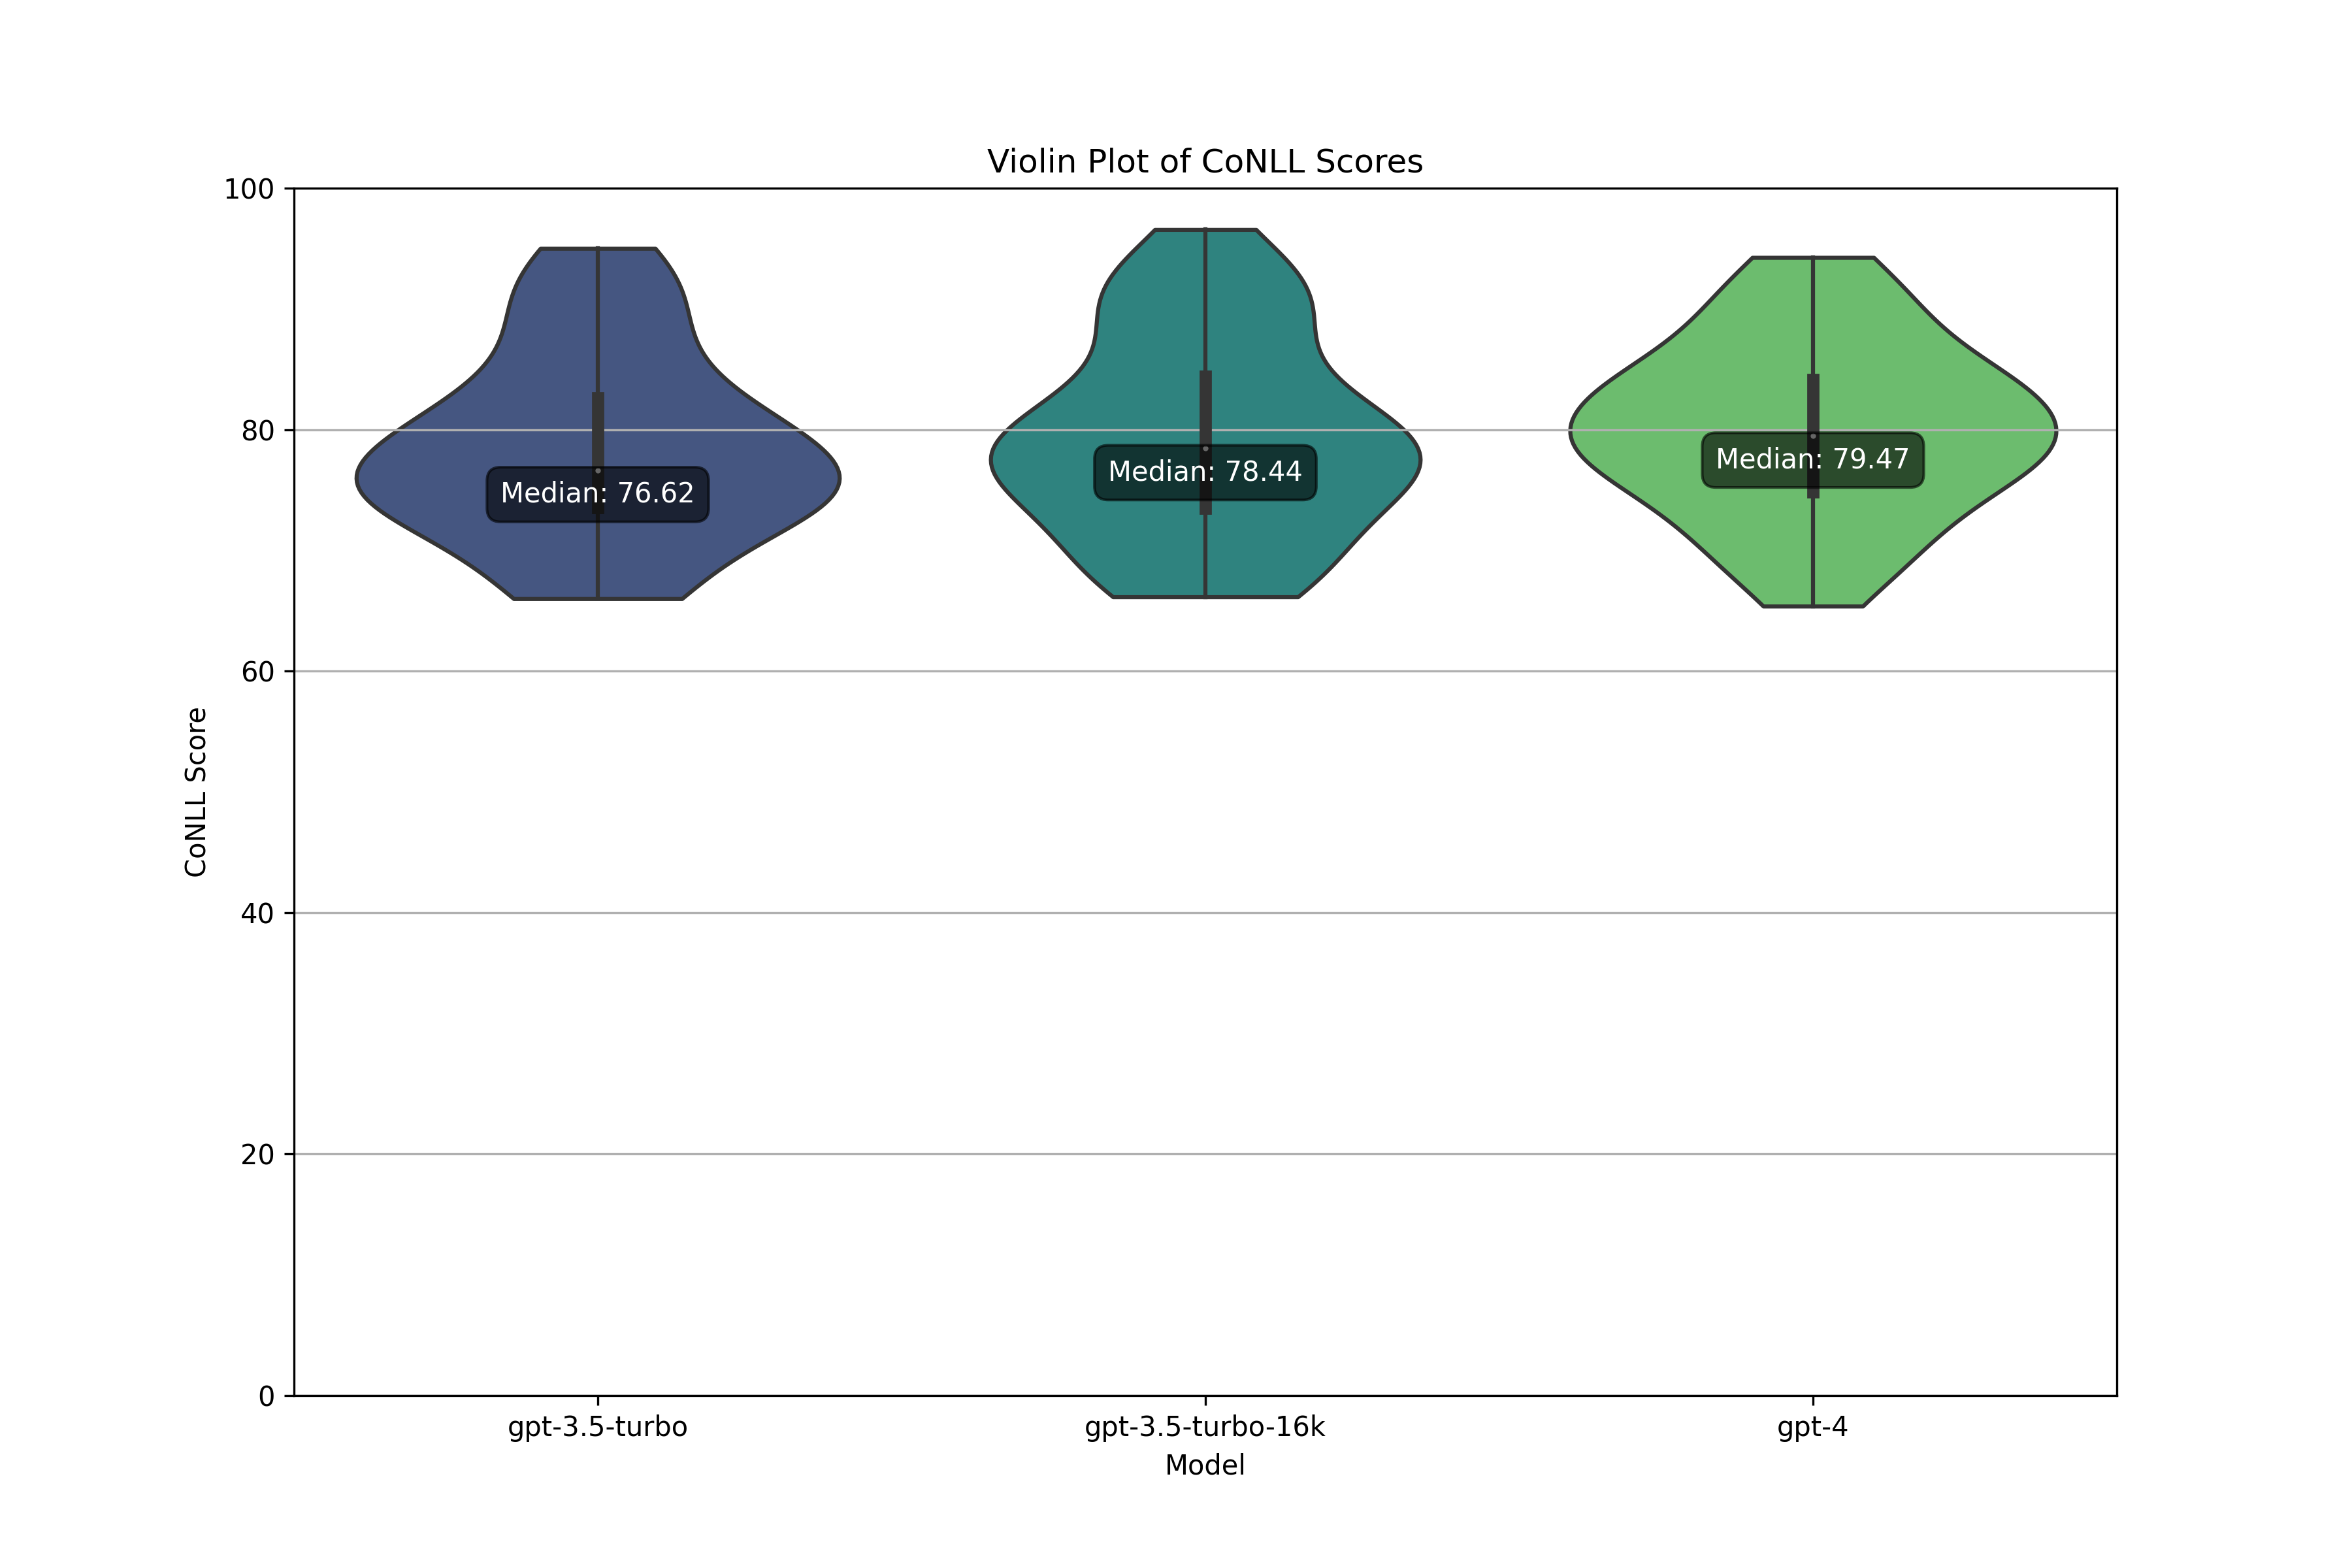
\includegraphics[width=14cm]{images/conll-score.png}
  \end{tabular}
  \caption[Distribution of CoNLL Score]{Violin plot of CoNLL scores for all three GPT models}\label{fig:violin-conll}
\end{figure}

\subsection{Estimation of CoNLL Score}
We observe that the CoNLL scores depend upon four primary factors: 
    \begin{enumerate}
        \item Topic: Our experiments revealed that papers from certain disciplines performed better — Logic is easier than NLP, with Astronomy and Mathematics following far behind. The underlying reason for this might be the training data, but due to the not-so-open nature of OpenAI, it is impossible to verify this. Moreover, the inherent nature of Language Models struggling with Mathematics is perhaps another reason GPT suffered in Mathematics papers.
        
        \item Model: The hierarchy is clear — GPT4 outperformes GPT-3.5-16k, which in turn surpasses GPT-3.5. 

        \item Ambiguity depends on the total number of discrete identifiers in a given paper. For example, in the formula $x = \frac{-b \pm \sqrt{b^2 - 4ac}}{2a}$ there are 4 identifiers, $x$, $a$, $b$, and $c$. The lower the number of identifiers, the better a model typically performs, as there are fewer distinctions to be made.
        
        \item Obscurity: This is estimated using the interquartile range of a given identifier's occurrences, focusing solely on the middle quartile and disregarding the outliers. From the same example of the quadratic equation of $x = \frac{-b \pm \sqrt{b^2 - 4ac}}{2a}$, $x$ and $c$ are repeated once but $a$ and $b$ are repeated twice. The rationale for focusing on the middle 40-percentile range is twofold. First, due to their limited occurrences, identifiers that appear infrequently (in the bottom 30th percentile) are generally easier for GPT to disambiguate. Second, persistent identifiers (in the top 30th percentile) may challenge annotation. However, our annotation approach results in a cascading effect that minimises its impact on the CoNLL score. Therefore, the identifiers falling within the middle 40-percentile truly contribute to the level of Obscurity. This subset is the primary focus when estimating the CoNLL score for annotation accuracy.
    \end{enumerate}

%% Rune: The creation of this formula needs to be more motivated (at all!) in the text.
The last three variables help us devise a robust mathematical formula that can be used to quickly estimate the actual CoNLL score:
%, with the computation process detailed in Figure \ref{fig:conll-estimation}.
%\clearpage

%\begin{figure}[htpb]
  \begin{equation}
      \text{conll\_score} \simeq \text{intercept} - \frac{2 \times \text{total\_concepts}}{5} - \frac{\text{occur\_iqr}}{5}
  \end{equation}\label{eq:1}
%  \caption[CoNLL Estimation]{Estimate the CoNLL Score for NLP Papers}
  \label{fig:conll-estimation}
%\end{figure}

In the equation above, the variables are defined as follows:
\begin{itemize}
  \item \textbf{conll\_score} is the CoNLL score being estimated (Domain dependent).
  \item \textbf{intercept} is the y-axis intercept, which depends on the model. GPT-3.5~=~93, GPT-3.5-16k~=~95, GPT-4~=~97. (Model)
  \item \textbf{total\_concepts} is the total number of concepts in the paper (Ambiguity).
  \item \textbf{occur\_iqr} represents interquartile, middle 40-percentile (Obscurity).
\end{itemize}

Despite the limited sample size, preliminary results in Table \ref{tab:mse-r2} demonstrate the potential of this predictive model. The formula's estimation Mean Square Error and R2 Score are shown. Since there were only 18 papers in hand for NLP, getting better results took much work. %%Rune: Was this not tested on papers from other domains? Are the intercepts specific to NLP papers?
Figure \ref{fig:esimated-conll} shows the visualisation of our novel formula on a 3D plane.

\begin{figure}[htpb]
  \centering
  \subfloat[Angled View]{
    \begin{tabular}{c}
  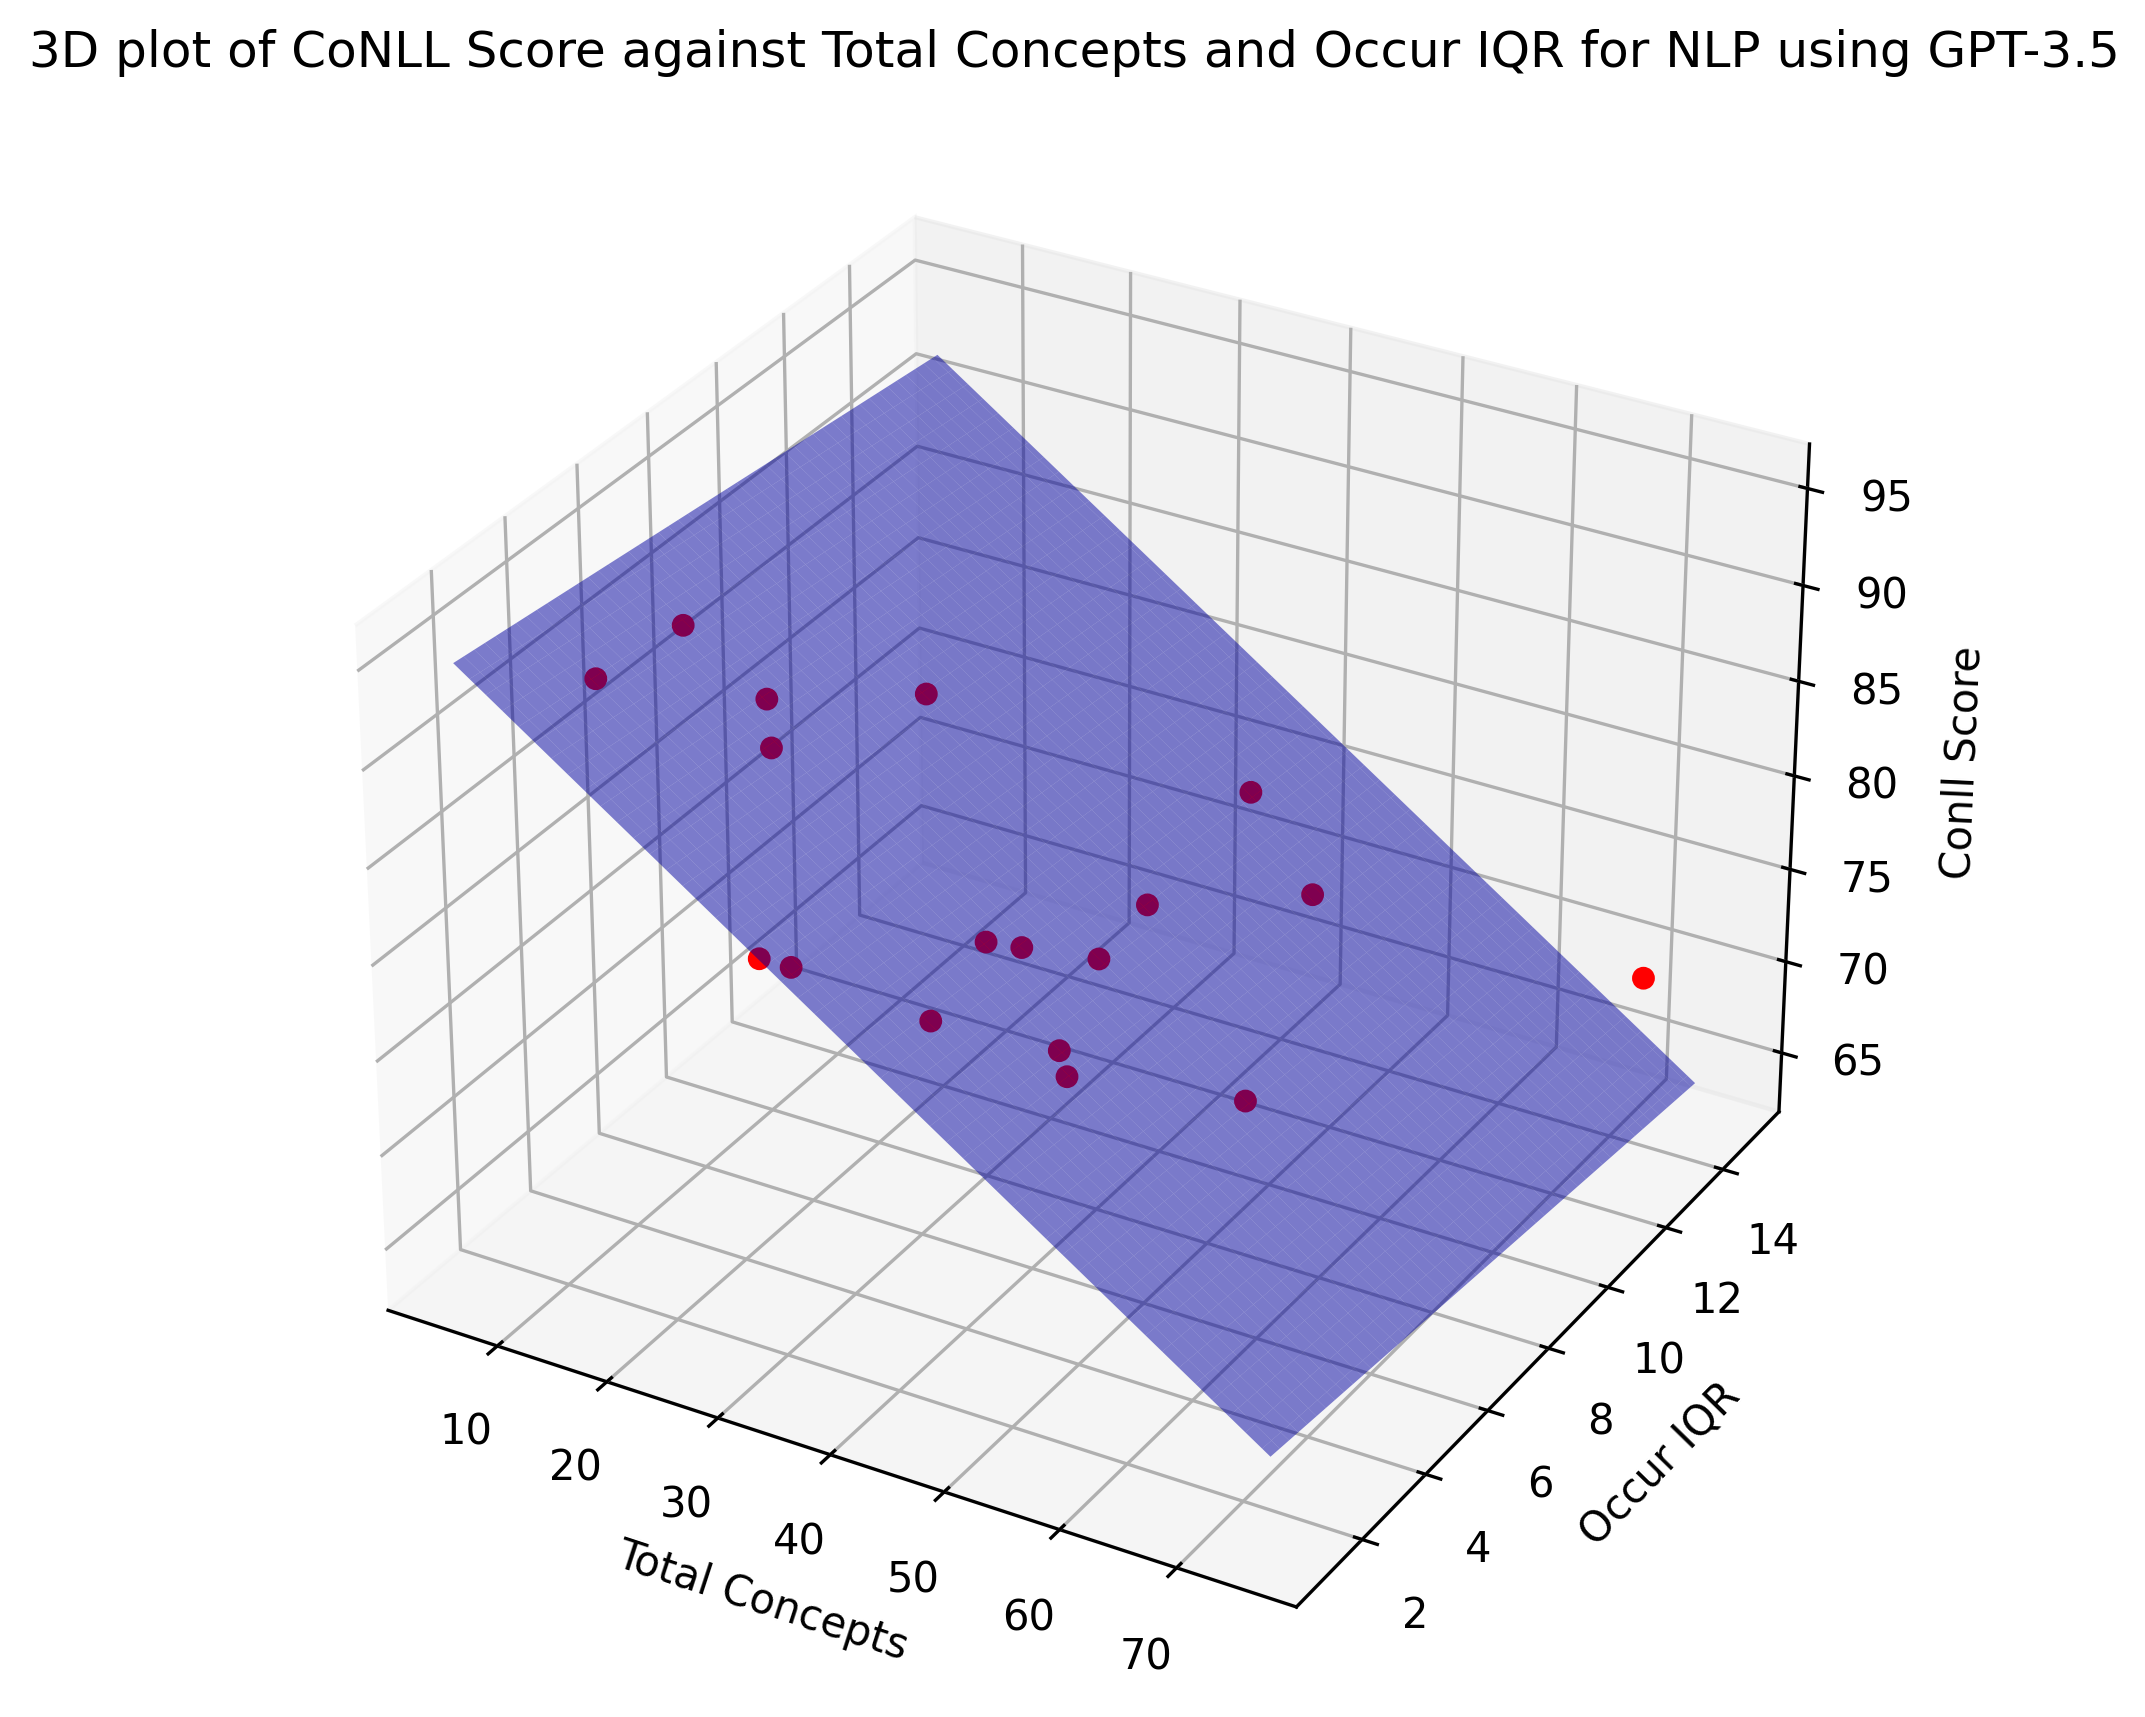
\includegraphics[width=11cm]{images/estimated-conll.png}
  \end{tabular}
  }
  \quad 
  \subfloat[Side view]{
    \begin{tabular}{c}
  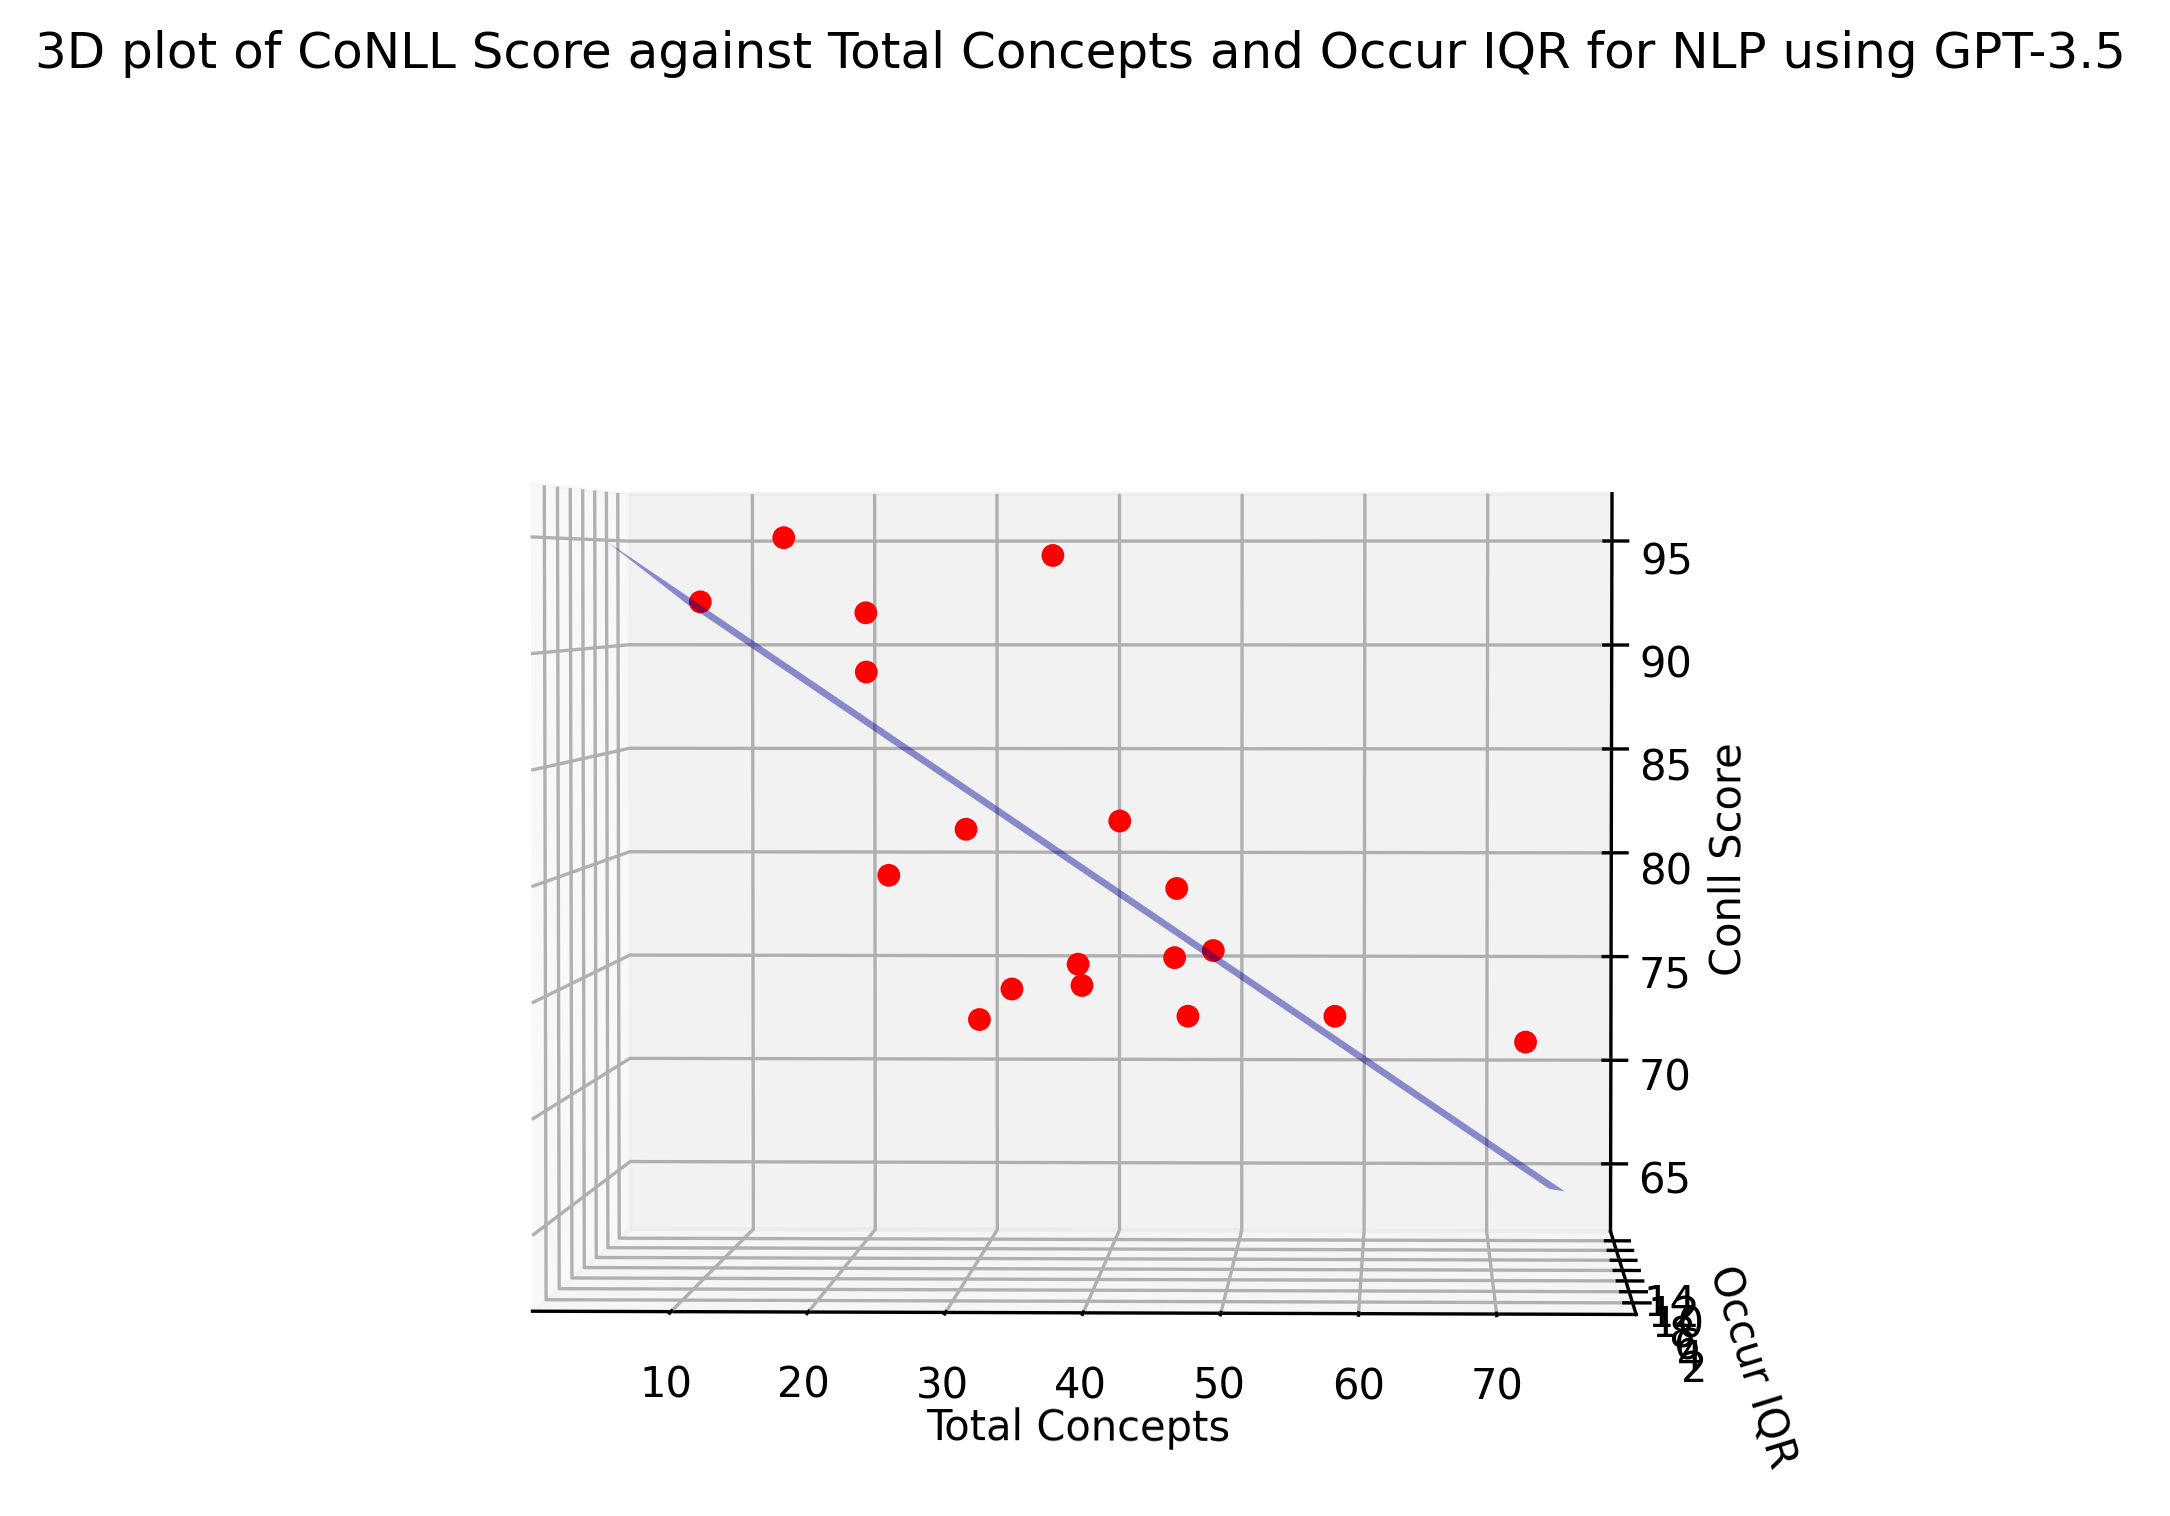
\includegraphics[width=11cm]{images/estimated-conll-2.png}
  \end{tabular}
  }
  \caption[CoNLL Score Estimation]{3D Visualisation of the CoNLL Score Estimation Formula}\label{fig:esimated-conll}
\end{figure}


\begin{table}[h]
    \centering
    \begin{tabular}{lrr}
        \hline
        Model & Mean Square Error & R2 Score \\
        \hline
        GPT-3.5-turbo & 35.636 & 0.136 \\
        GPT-3.5-16k-turbo & 25.936 & 0.371 \\
        GPT-4 & 26.386 & 0.360 \\
        \hline
    \end{tabular}
    \caption{Mean Square Error and R2 Score of the Estimation Formula}
    \label{tab:mse-r2}
\end{table}

\subsection{Coverage of Annotation}

The coverage of annotation refers to the proportion of the paper that the LLMs successfully annotated. Consistent with the CoNLL results, GPT-4 again consistently outperforms the other two GPT models. GPT-3.5-16k, in contrast, had lesser coverage than GPT-3.5 due to the 16k model's instability and propensity for repetition death. %% Rune: What kind of death?
Figure~\ref{fig:violin-coverage} provides a visual representation of the coverage exhibited by all three models.

\begin{figure}[htpb]
  \centering
  \begin{tabular}{c}
  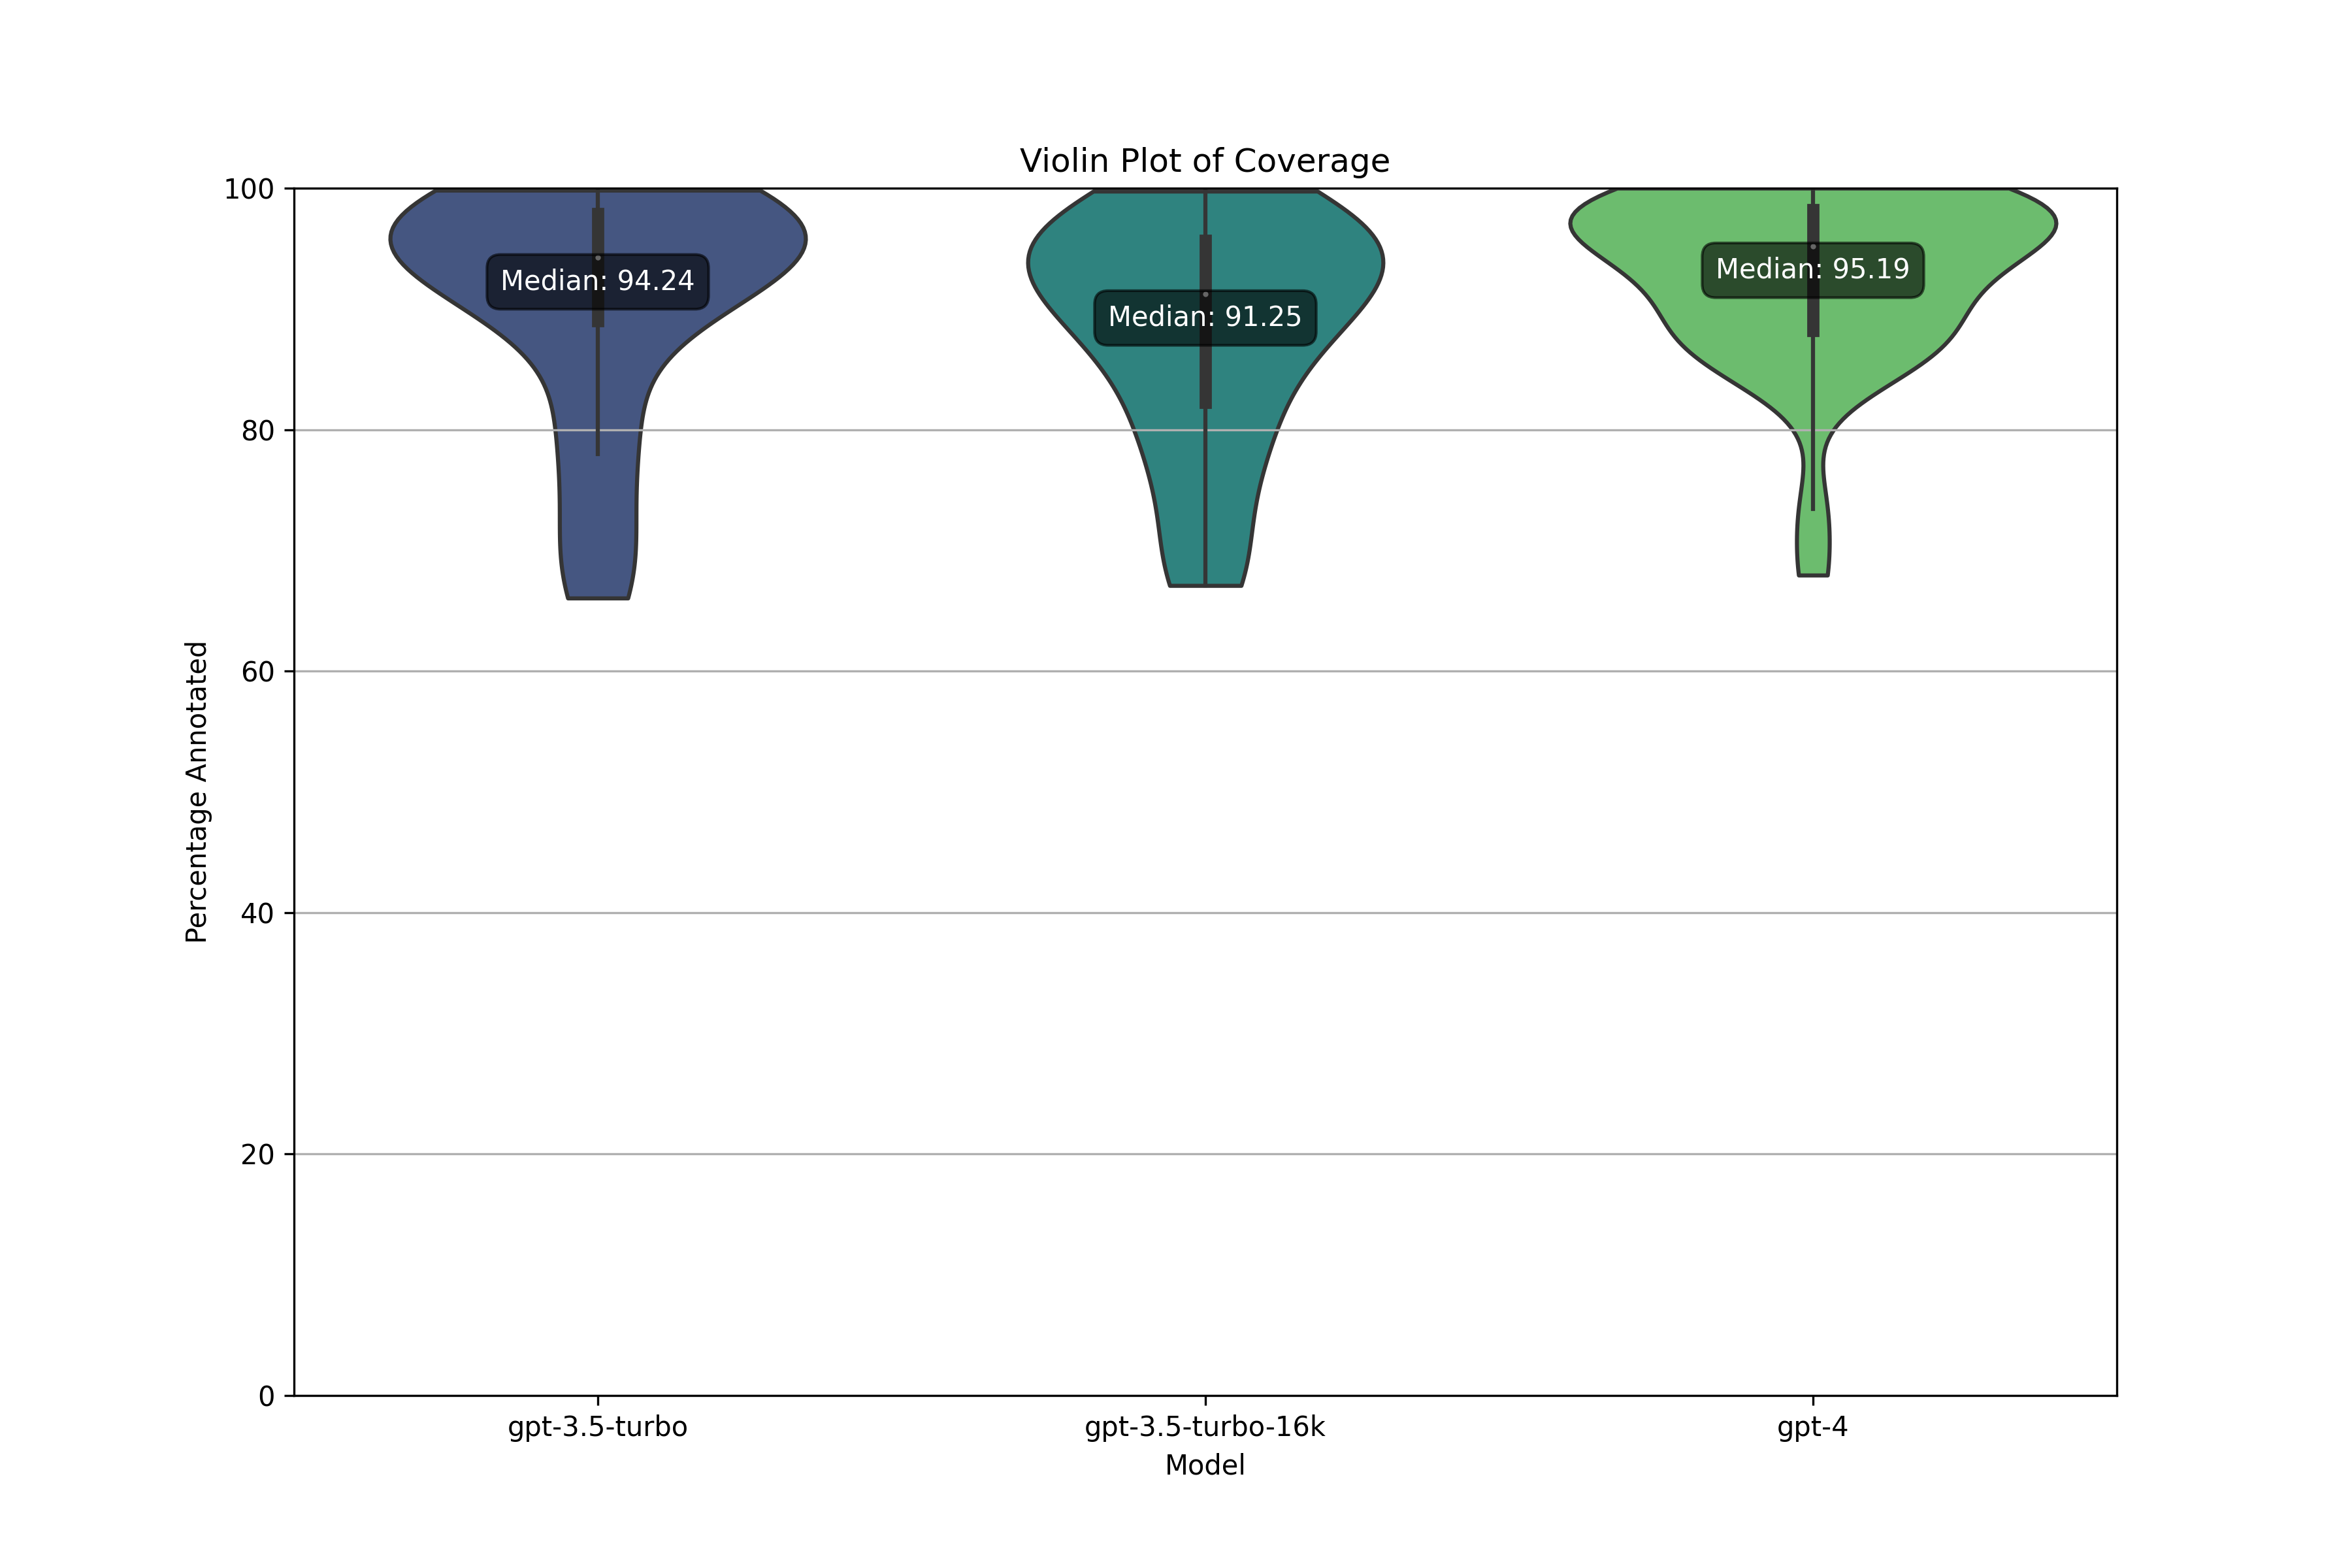
\includegraphics[width=14cm]{images/coverage.png}
  \end{tabular}
  \caption[Distribution of Coverage]{Violin plot of the Coverage of Annotations for all three GPT models}\label{fig:violin-coverage}
\end{figure}
 
\subsection{Semantic Accuracy}
%% TODO RUNE: Keep reading from here 1613, 13/9
Semantic accuracy provides a measure of the correctness of the annotations. We weighted it against the coverage to calculate a per paper-based total score. Because of the extensive difficulty of manually reviewing semantic accuracy, we evaluated five carefully picked papers representing various low/high CoNLL scores and lengths. As shown in Figure \ref{fig:violin-semantic}, GPT-4 consistently outperformed all the other models by a significant margin. There were a few papers where GPT-4 achieved a 100\% semantic accuracy, but weighing it with coverage brings it down to 98\%. GPT-4's worst performance is almost as good as the best performances of other models, making it superior. This comes as no surprise since GPT-4 is one of the largest (and most expensive) LLMs as of writing this thesis (late 2023).

\begin{figure}[htpb]
  \centering
  \begin{tabular}{c}
  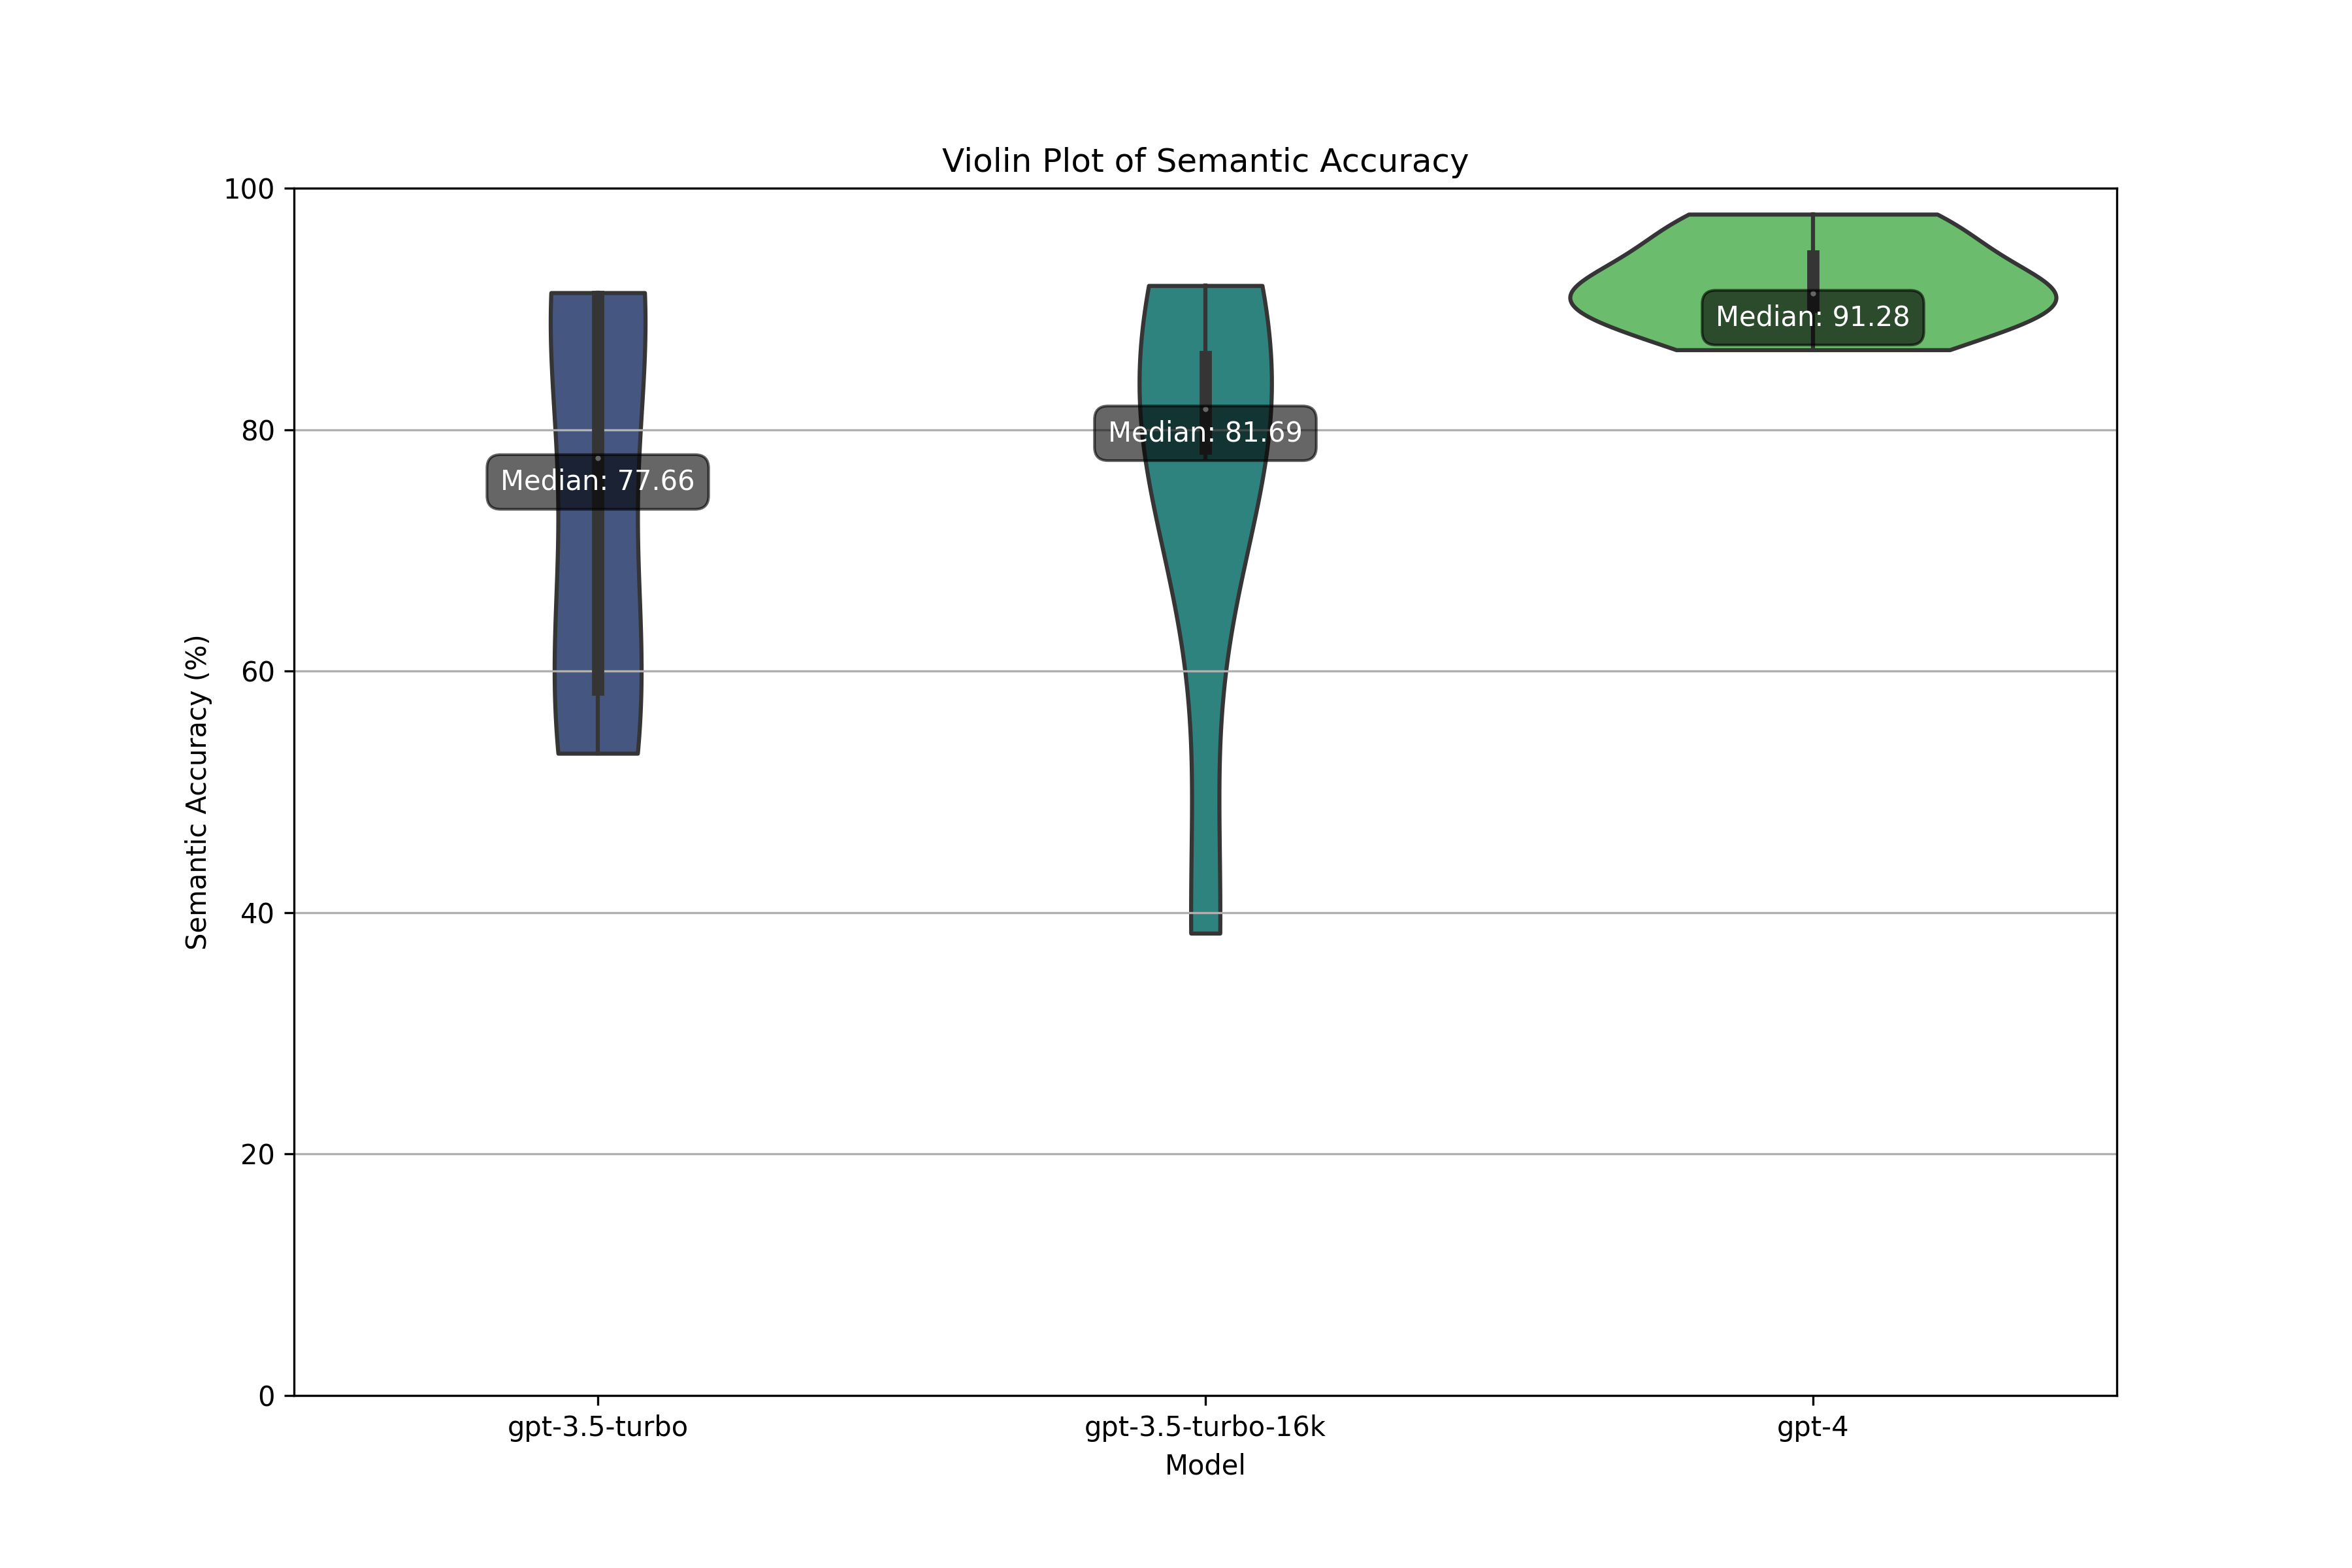
\includegraphics[width=14cm]{images/semantic-accuracy.png}
  \end{tabular}
  \caption[Semantic Accuracy]{Violin plot of the Weighted Semantic Accuracy of all GPT Models}\label{fig:violin-semantic}
\end{figure}

\subsection{Variance of the Results Data}

To account for these models' stochastic nature and measure our experiment's reproducibility and stability, we repeated the same experiment on one reference paper\footnote{\url{https://arxiv.org/pdf/2107.10832.pdf}}~\citep{singleton2021logic}. We ran the experiment four times, evaluating the variance in the CoNLL scores. GPT-3.5 and GPT-4 proved monumentally stable, whereas GPT-3.5-16k, a newer model, still exhibited volatility issues. These outcomes are displayed in Figure \ref{fig:violin-variance}.

\begin{figure}[htpb]
  \centering
  \begin{tabular}{c}
  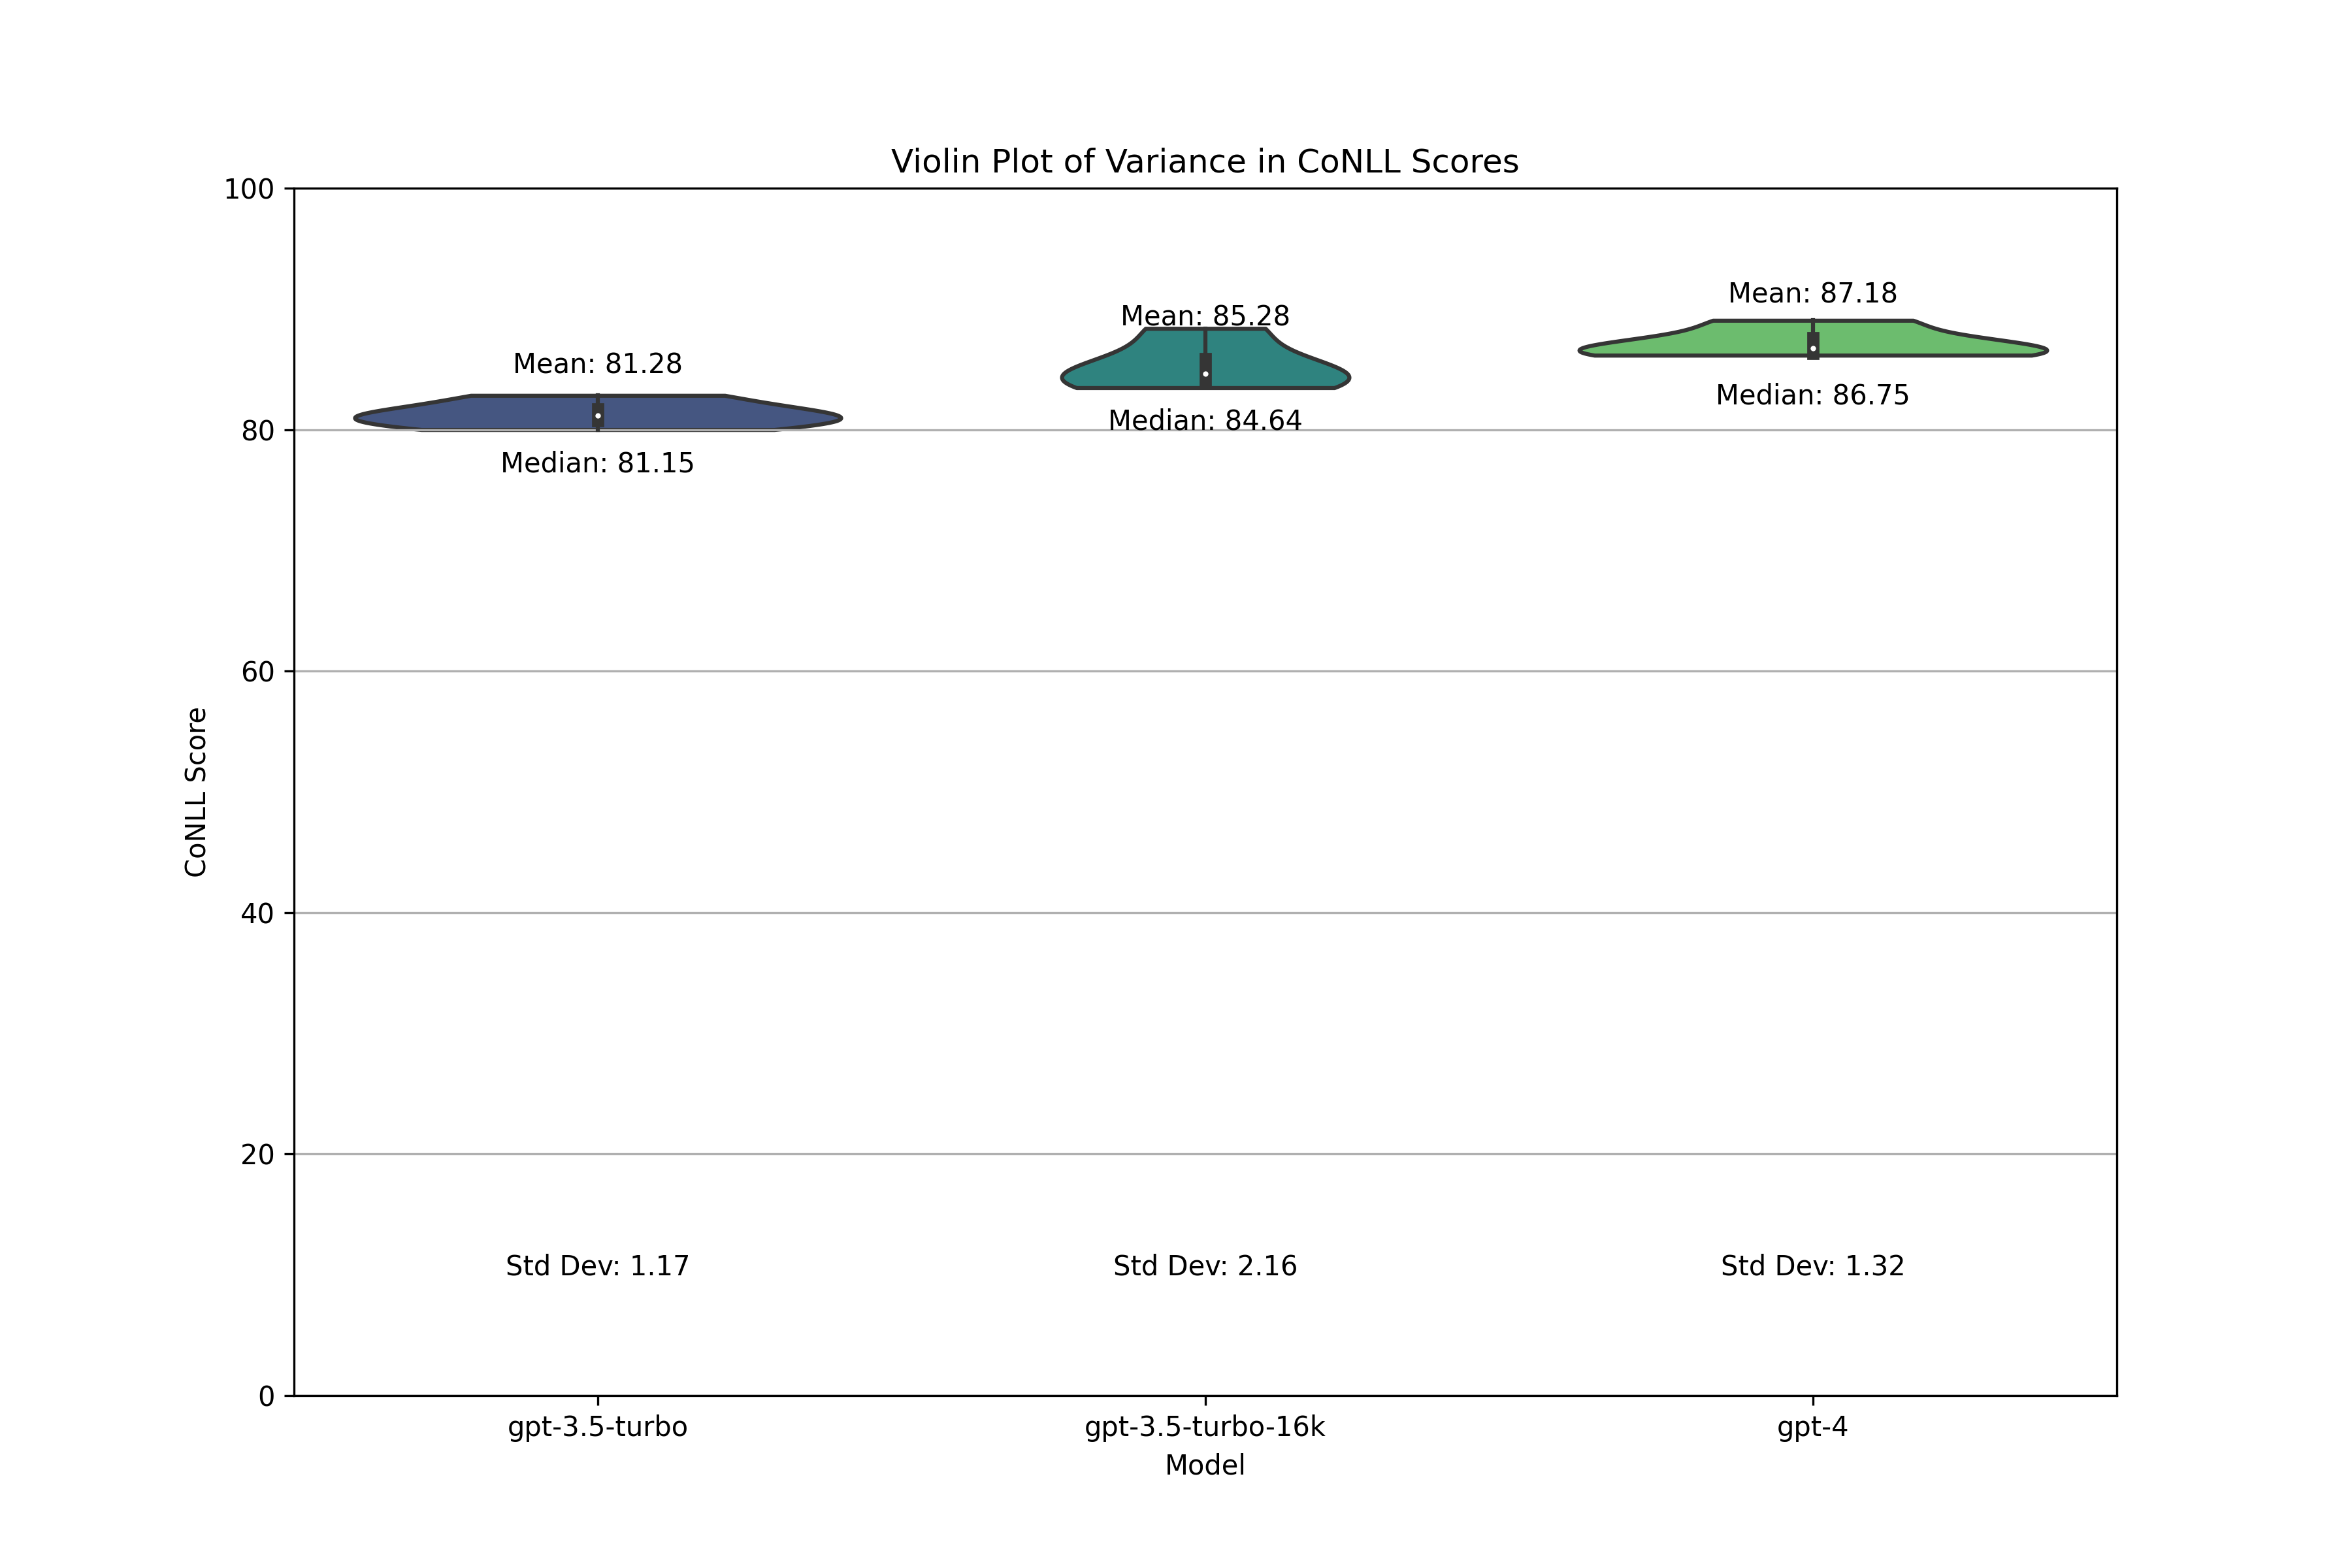
\includegraphics[width=14cm]{images/variance-conll.png}
  \end{tabular}
  \caption[The variance]{Violin plot of the variance in CoNLL scores for the same paper annotated four times}\label{fig:violin-variance}
\end{figure}

\subsection{Running Time and Costs}

The financial aspects of utilising GPT models are quantified through token usage. A comprehensive visualisation of the average costs and time durations for our experiments is provided in Figure \ref{fig:gpt-cost-anal}. It is crucial to note that the length of the paper influences both the cost and the time needed. To offer a more standardised comparison, we present the costs normalised per 1,000 annotations in Figure \ref{fig:gpt-relative-cost}.

Another pivotal dimension is the trade-off between cost and time efficiency. While the ideal scenario would be to minimise both, practical constraints often make this challenging. This relationship is further explored in Figure \ref{fig:gpt-time-v-cost}.
GPT-3.5 emerged as the most cost-effective and time-efficient option among the GPT models evaluated. This efficiency is attributable to OpenAI's competitive token pricing and additional optimisations (for ChatGPT). Conversely, GPT-4 incurred the highest expenses due to its elevated token costs. GPT-3.5 and GPT-4 demonstrated remarkable stability, contributing to their lower time expenditures. On the other hand, GPT-3.5-16k exhibited instability, leading to increased running time. %% Rune: This time, cost/instability is unclear to me.

\begin{figure}[htpb]
  \centering
  \subfloat[Average Cost of Annotation]{
    \begin{tabular}{c}
  \hspace*{-.25cm}
  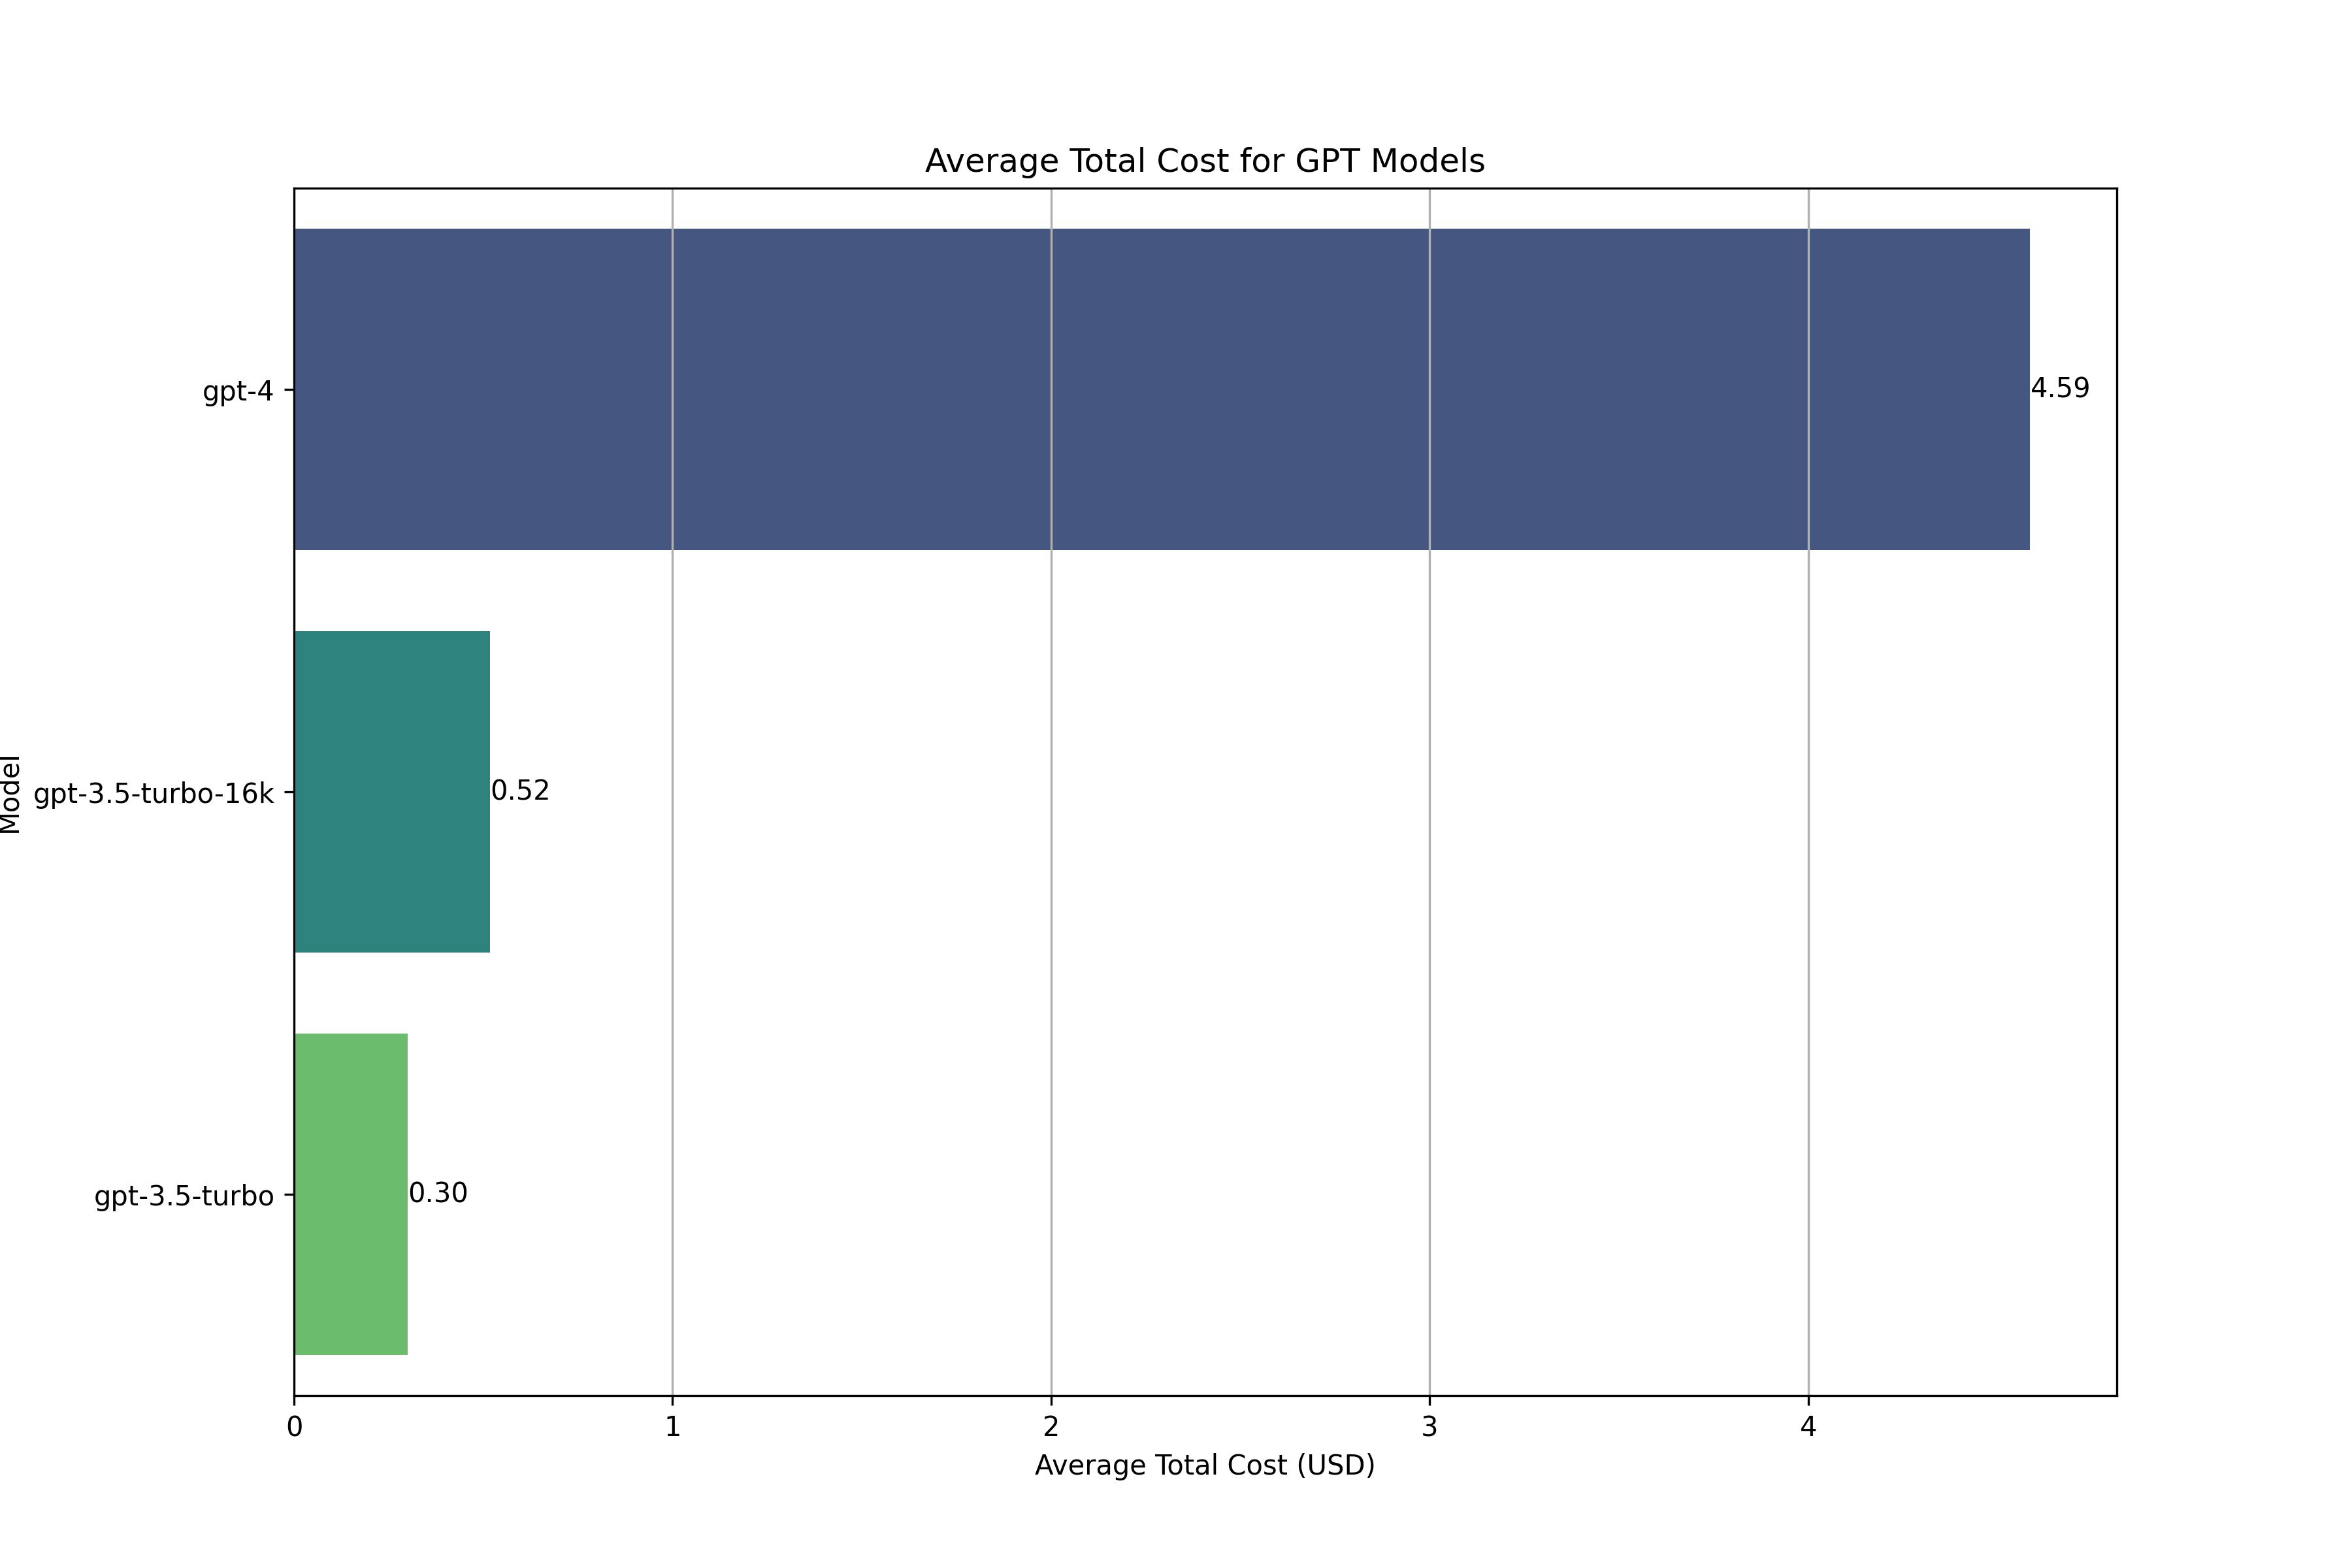
\includegraphics[width=11cm]{images/cost-gpt.png}
  \end{tabular}
  }
  \quad 
  \subfloat[Average Duration of Annotation]{
    \begin{tabular}{c}
  \hspace*{-1.5cm}
  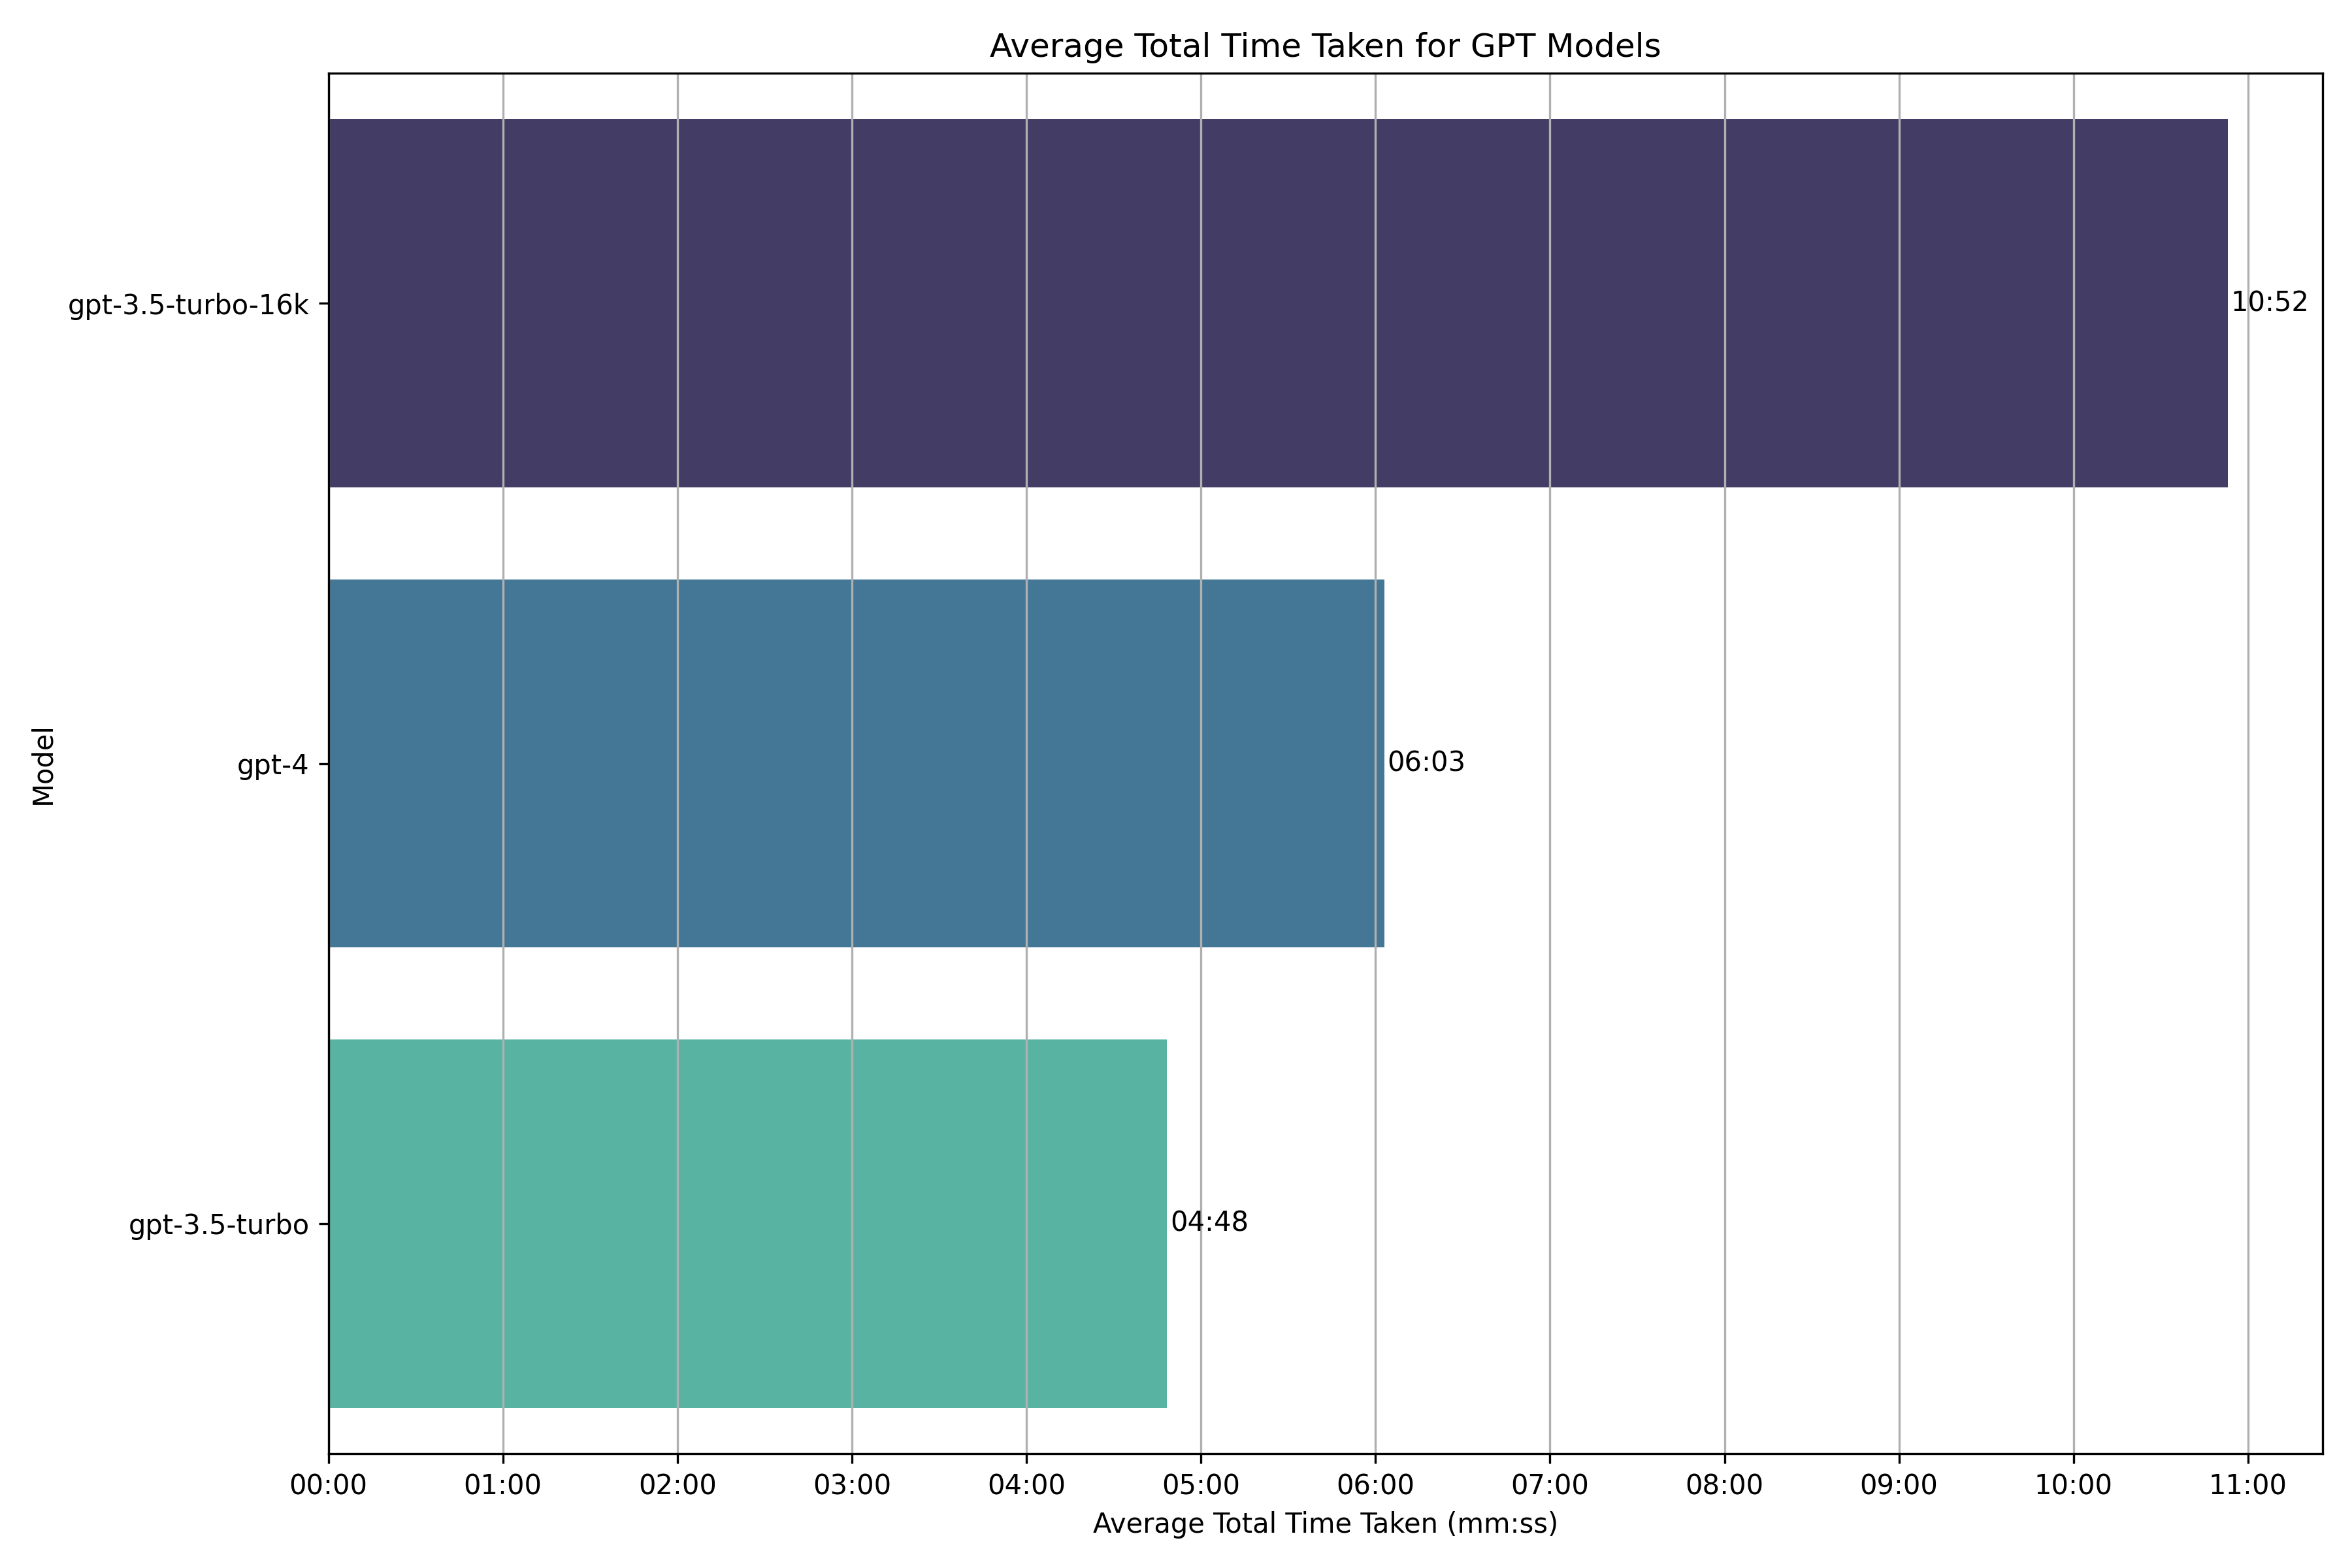
\includegraphics[width=10cm]{images/time-gpt.png}
  \end{tabular}
  }
  \caption[Cost Analysis]{Cost and Time Usage of Annotations}\label{fig:gpt-cost-anal}
\end{figure}

\begin{figure}[htpb]
  \centering
  \subfloat[Average Cost per 1000 Concept]{
    \begin{tabular}{c}
  %\hspace*{-.25cm}
  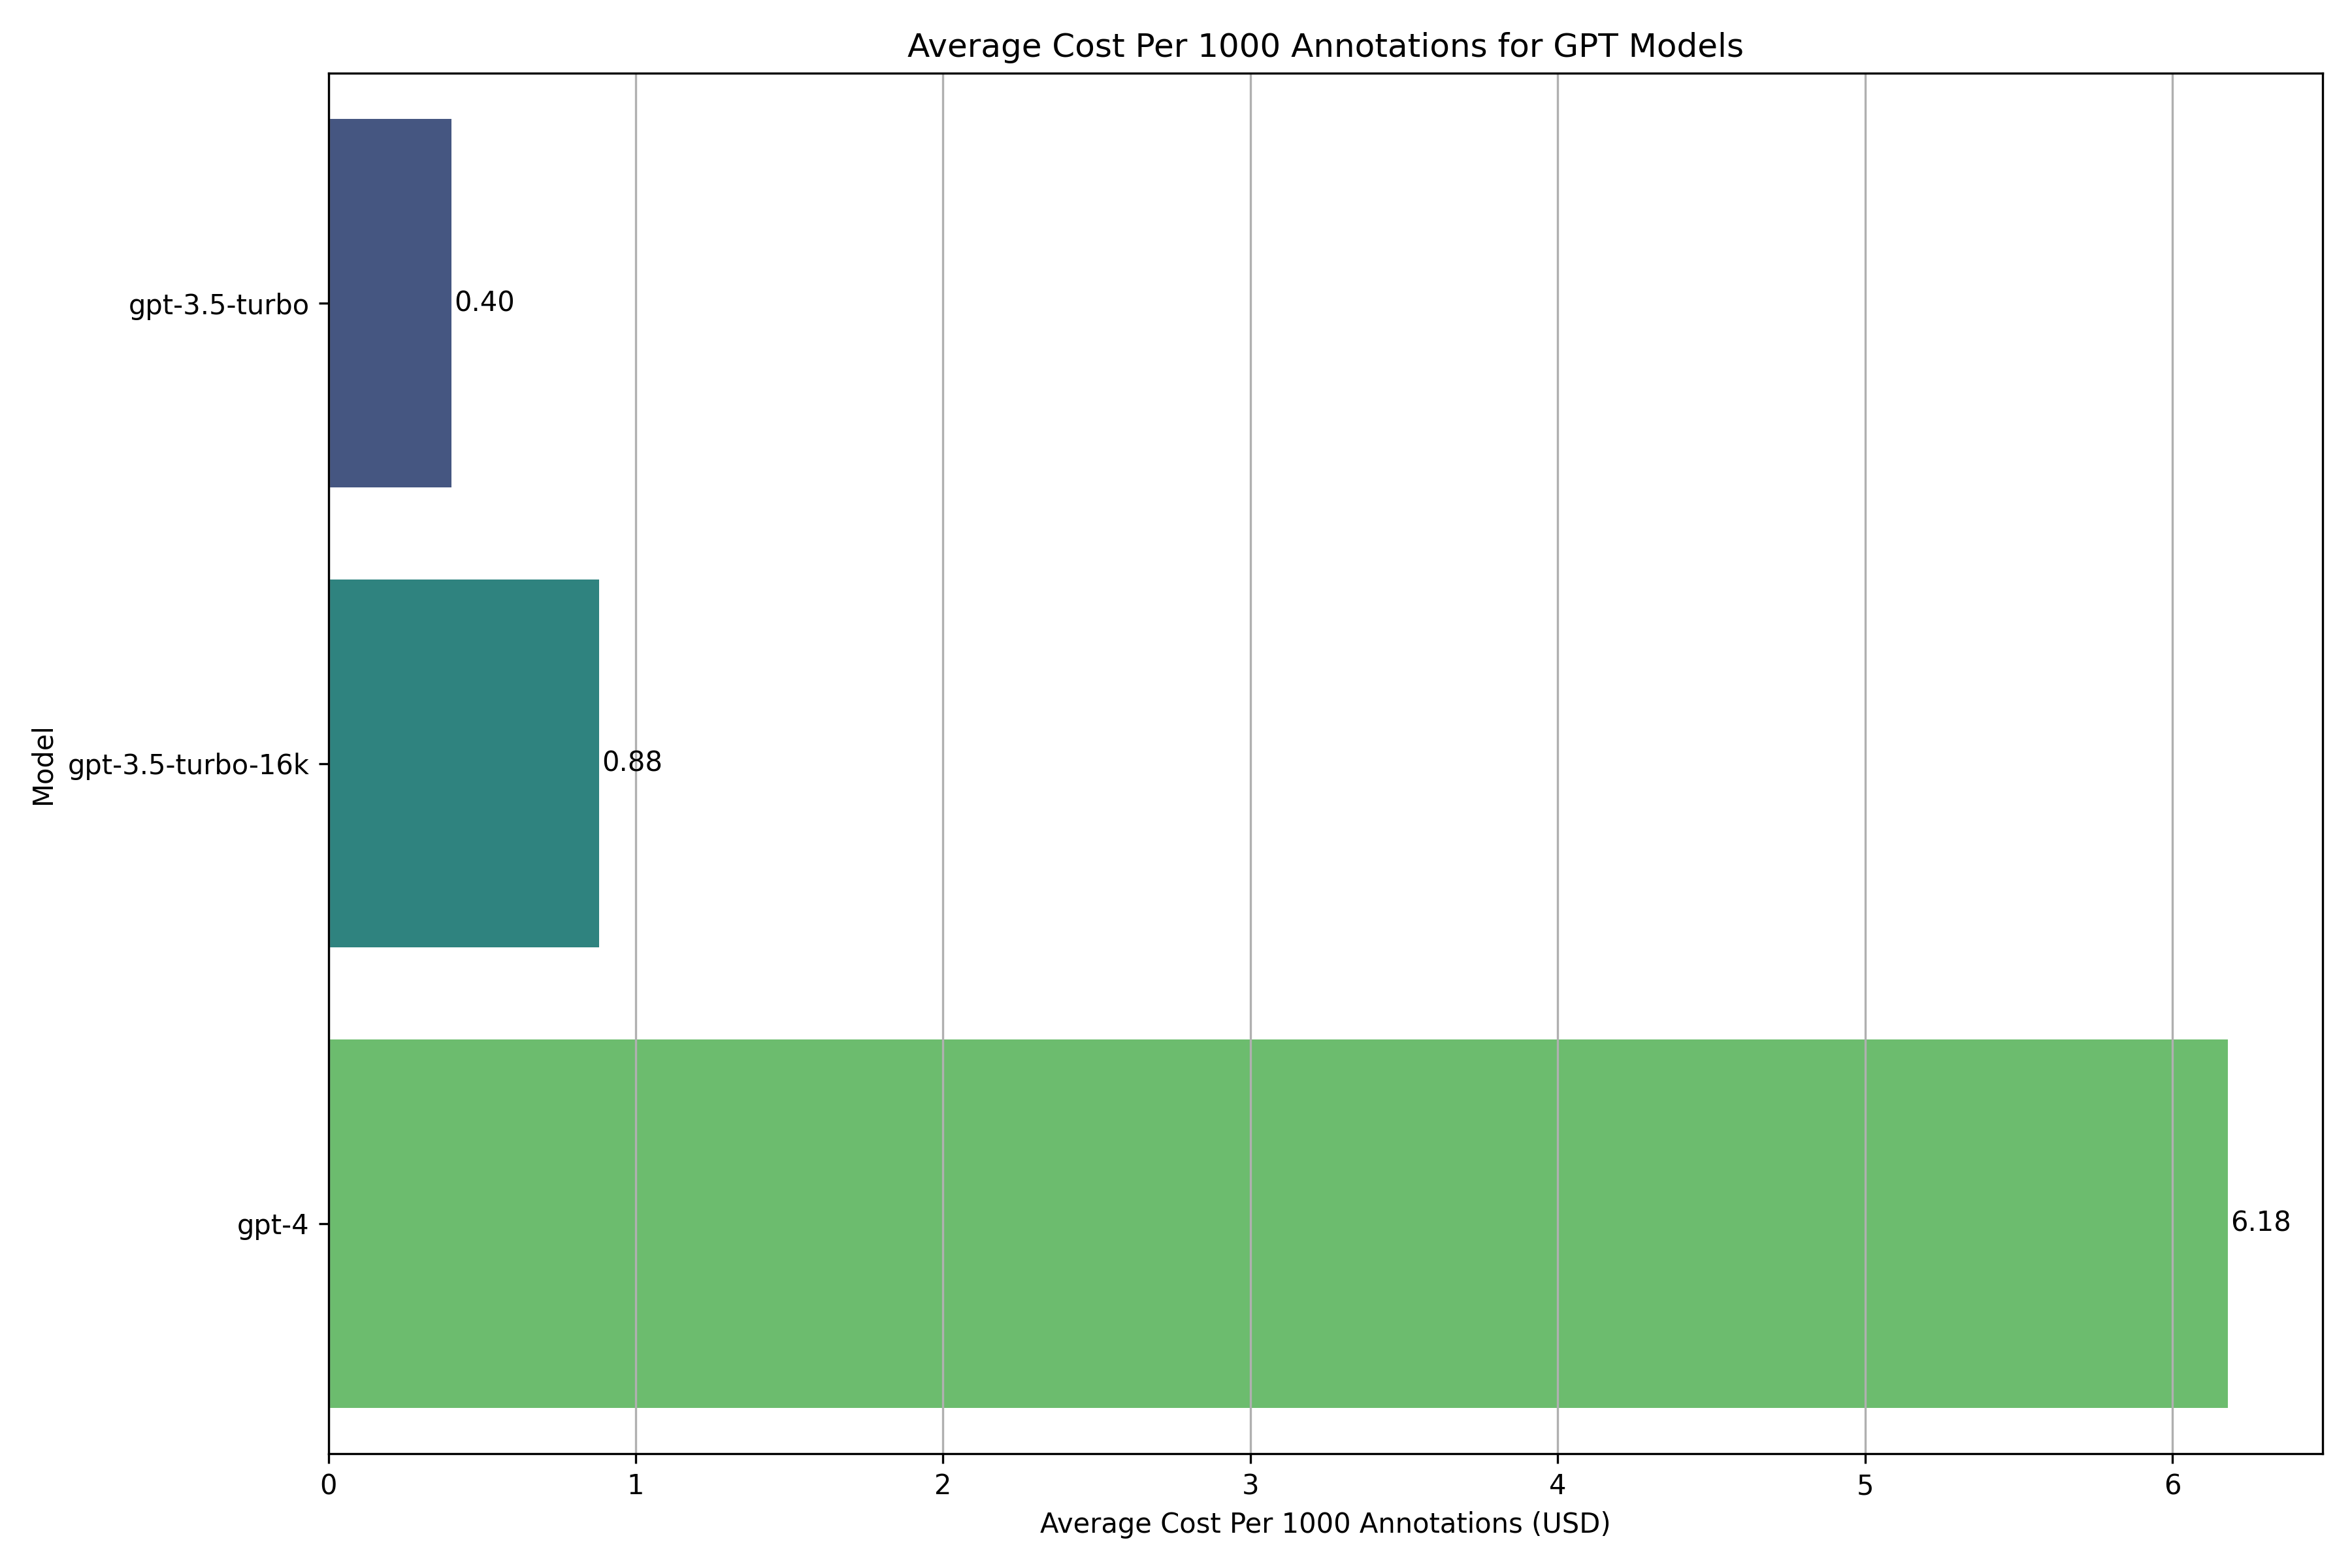
\includegraphics[width=11cm]{images/gpt-relative-cost.png}
  \end{tabular}
  }
  \quad 
  \subfloat[Average Duration per Concept]{
    \begin{tabular}{c}
  %\hspace*{-1.5cm}
  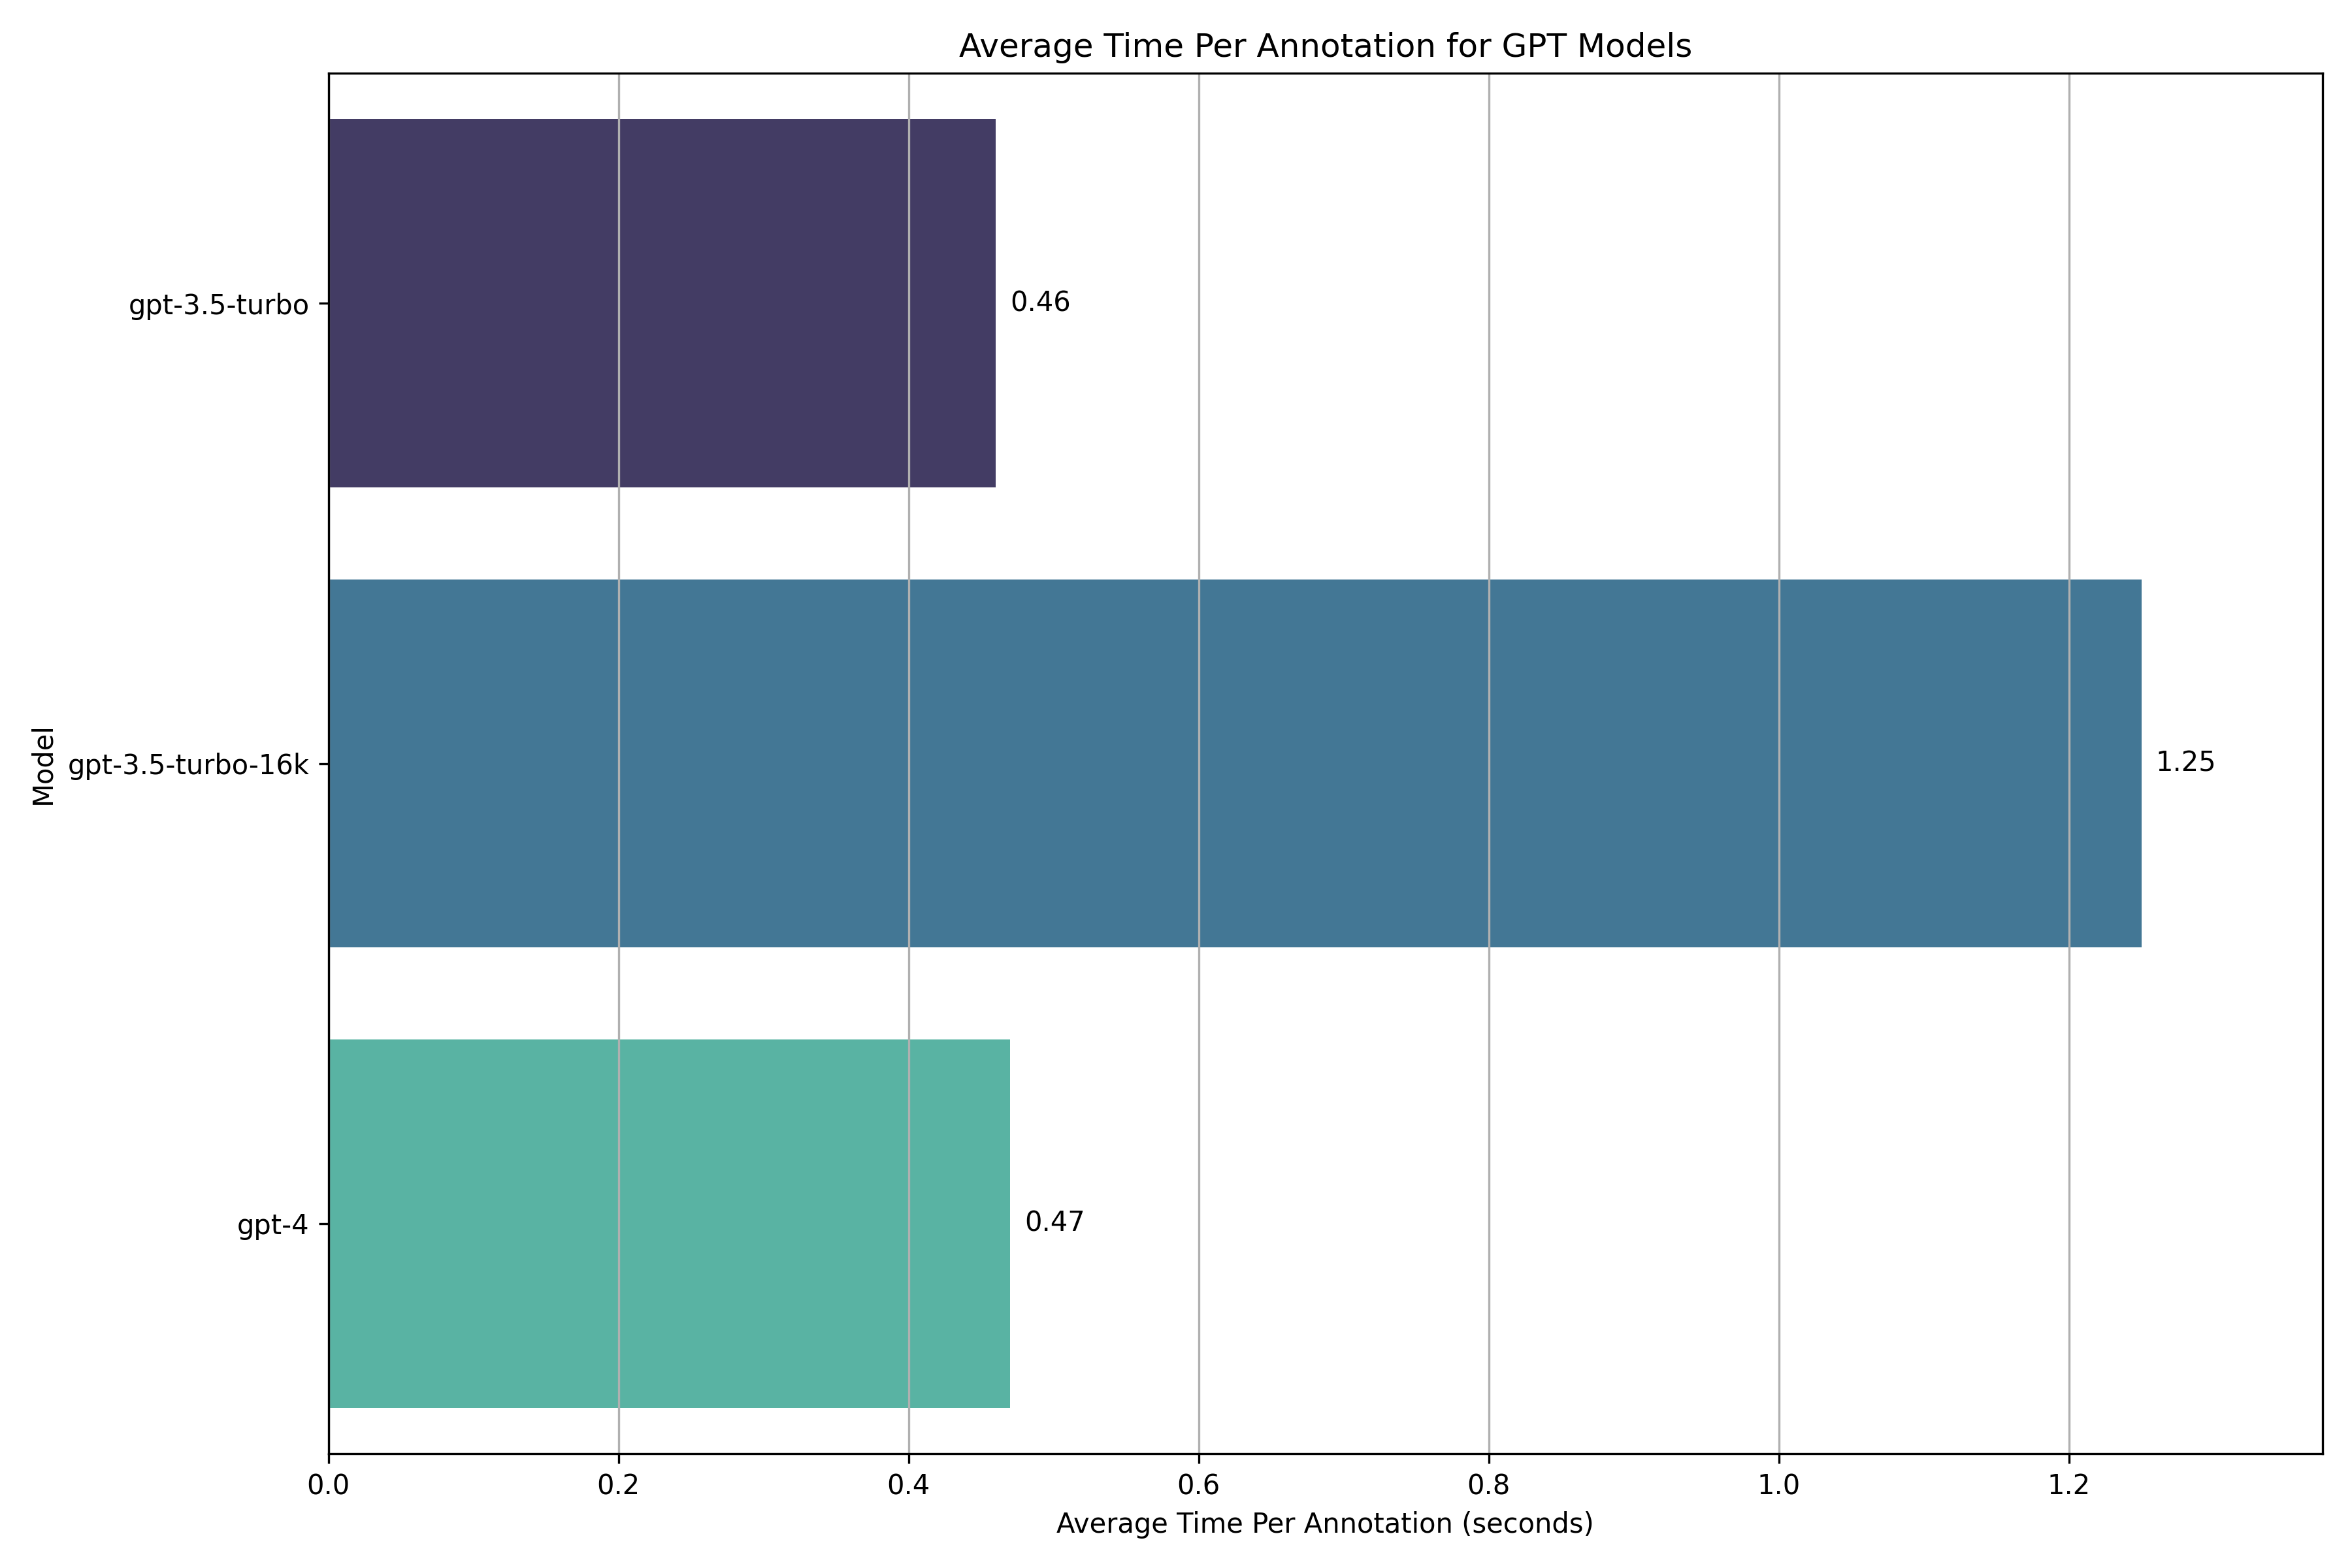
\includegraphics[width=10cm]{images/gpt-relative-time.png}
  \end{tabular}
  }
  \caption[Time Cost Analysis]{Cost and Time Usage of Automation}\label{fig:gpt-relative-cost}
\end{figure}

\begin{figure}[htpb]
  \centering
  \begin{tabular}{c}
  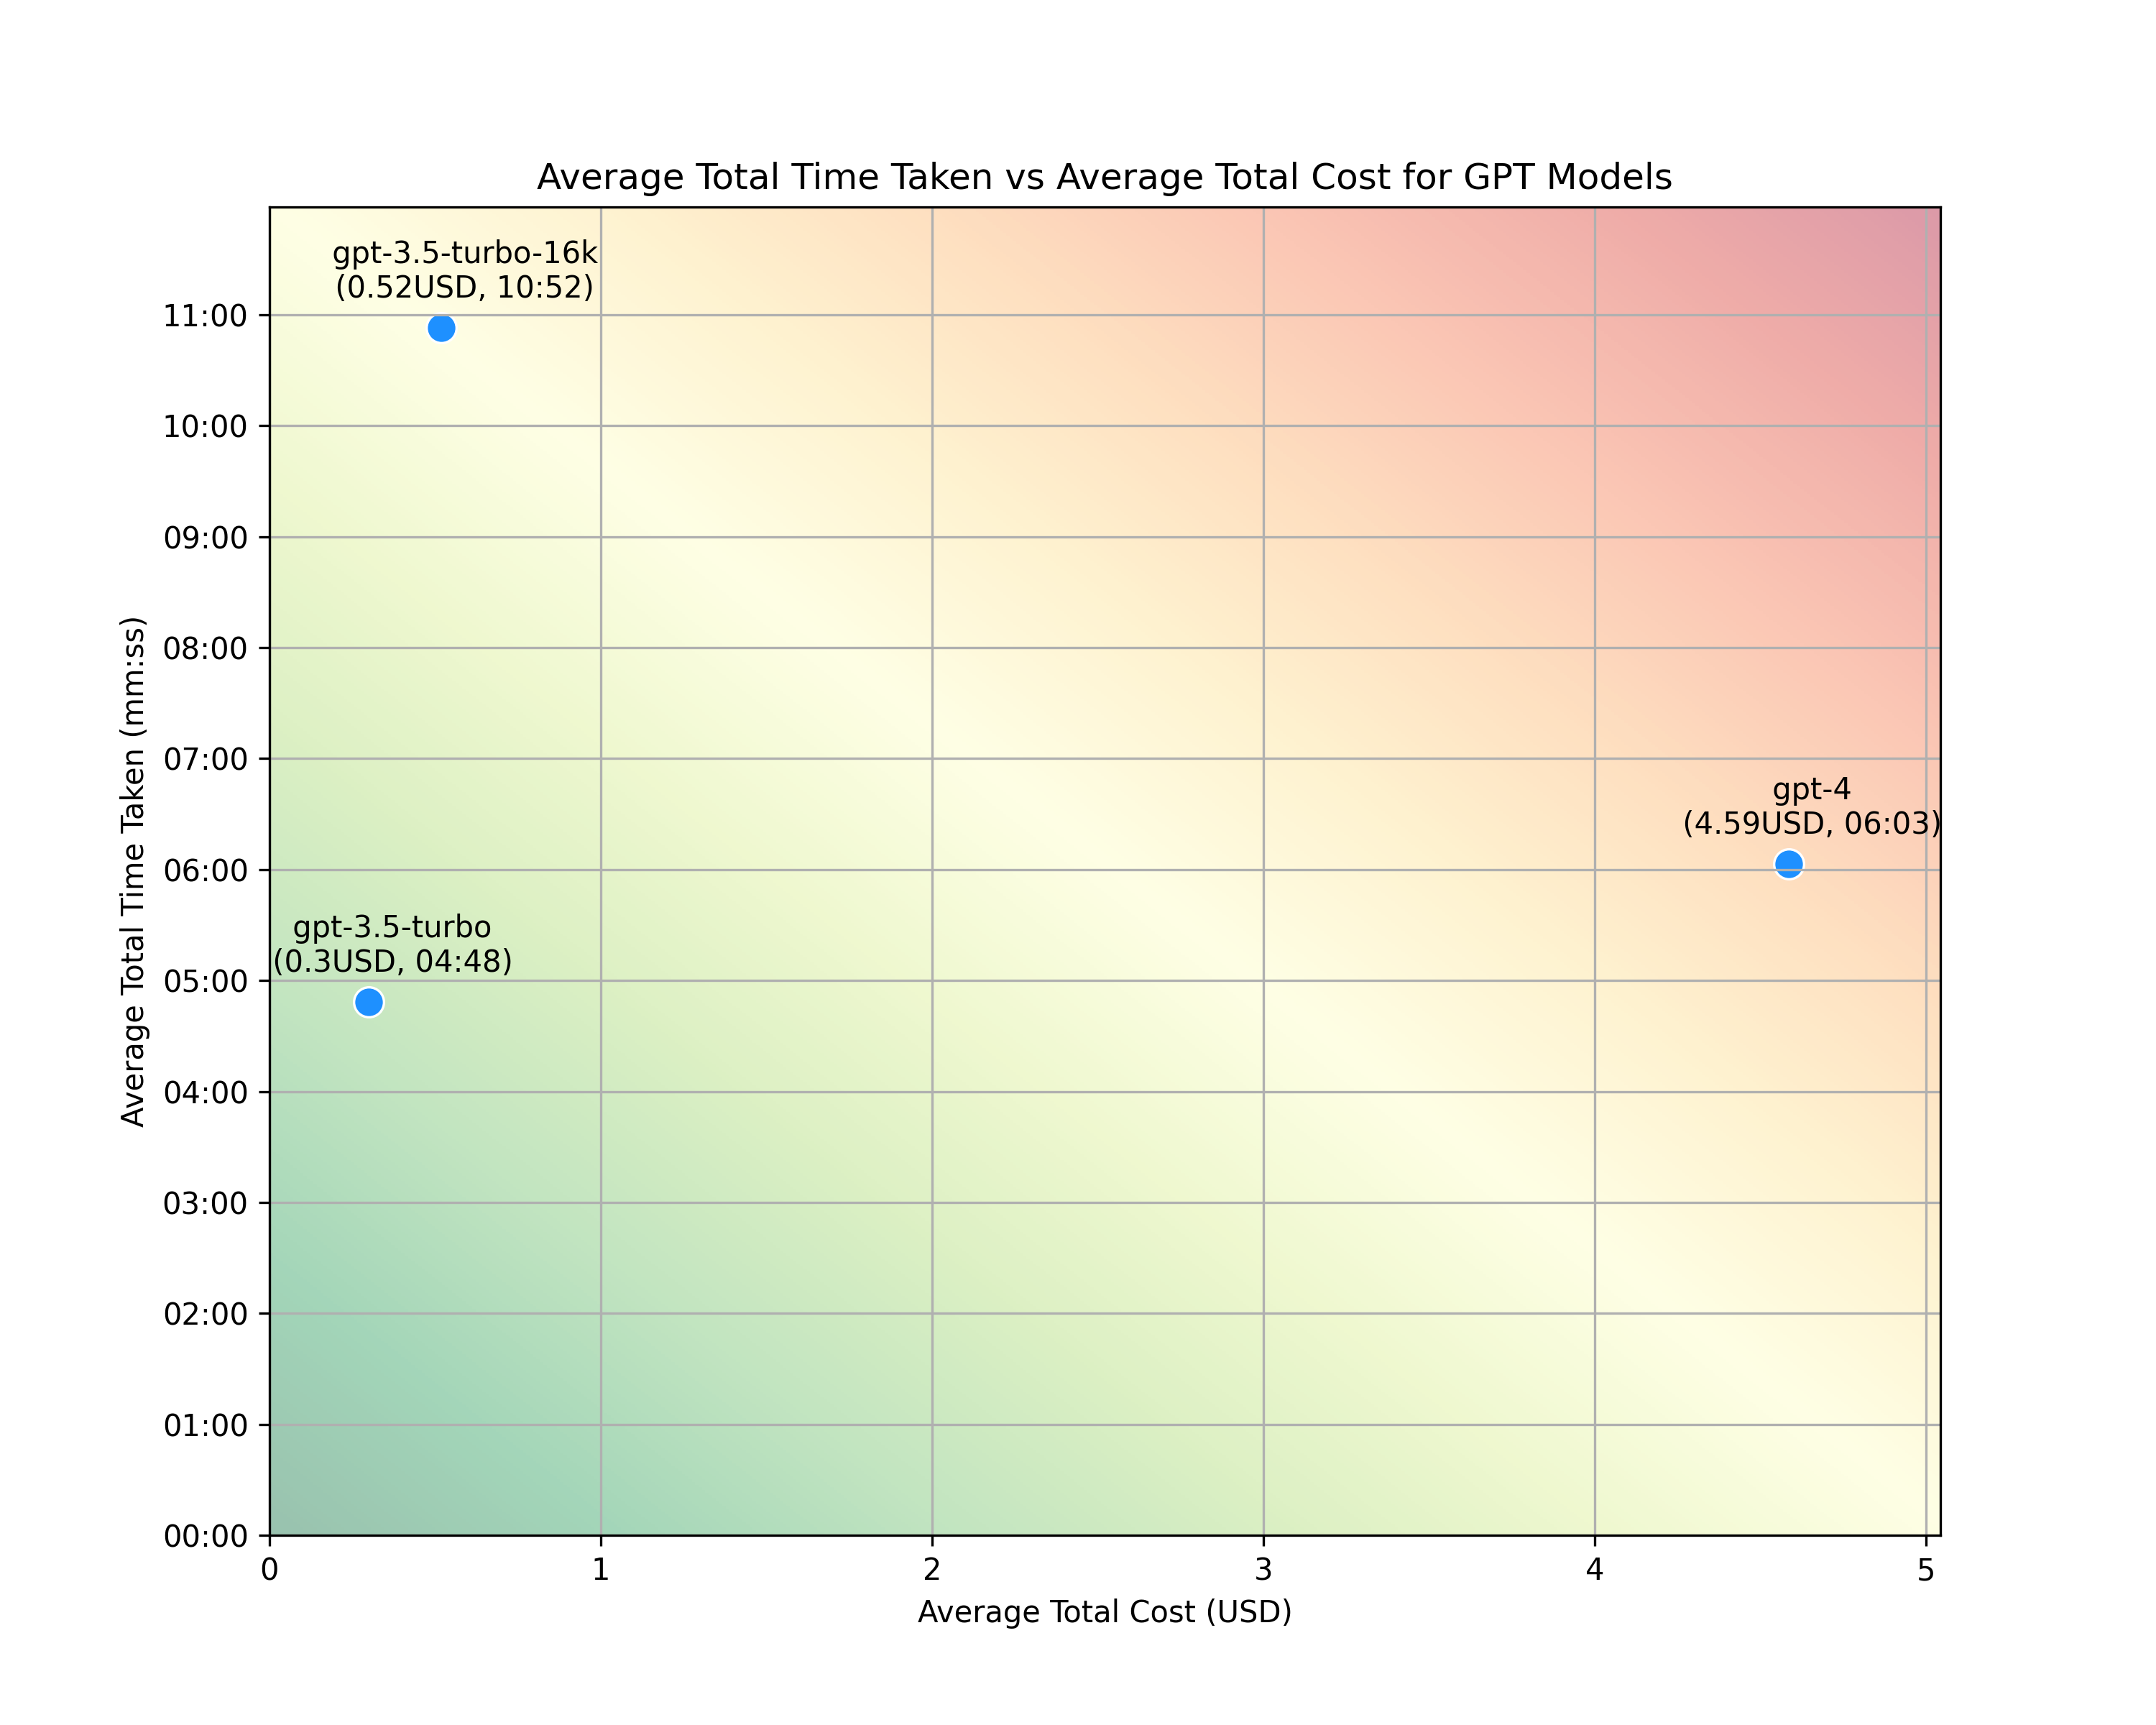
\includegraphics[width=14cm]{images/gpt-time-v-cost.png}
  \end{tabular}
  \caption[Cost vs Time]{Scatter Plot of Average Cost vs Time Taken}\label{fig:gpt-time-v-cost}
\end{figure}


\section{Open Souce LLMs}

Next, we also thoroughly examined the annotations generated by the OpenSource Models. A smaller subset with 7 of the 40 papers selected by \citet{asakura2022building} was used as the ground truth for this analysis. Dictionaries and annotations were generated for these papers. The Open Source models varied drastically in terms of their performance. Among the two models we evaluated, Vicuna-33b lagged noticeably behind the GPT models in performance. This outcome is expected because Vicuna-33b operates on a comparably small 33-billion parameter architecture. However, it is noteworthy that a small-scale model still demonstrates a formula grounding capability.

Conversely, StableBeluga2 exhibited outstanding performance, nearly matching that of GPT-4. This is particularly impressive, considering that StableBeluga2 operates on only a 70-billion parameter framework, while GPT-4 is rumoured to have a staggering 1.8 trillion parameters. Moreover, StableBeluga2 consistently outperformed GPT-3.5 across multiple metrics. This superior performance is likely attributable to the specialised nature of StableBeluga2, designed as an "instruct" model, in contrast to GPT models that are general-purpose chat models not explicitly optimised for formula grounding.

\subsection{CoNLL Score}

Vicuna-33b struggled in several cases, even scoring zero in one instance, hinting at its inability to generate any meaningful dictionary for that paper. StableBeluga2, on the other hand, aptly managed to deliver performances that stood almost on par with the GPT models as illustrated in Figure \ref{fig:open-source-conll}. Despite this, GPT models maintained a discernible edge in disambiguation capabilities over their open-source counterparts. This advantage is likely attributable to the extensive training that GPT models undergo.

\begin{figure}[htpb]
  \centering
  \begin{tabular}{c}
  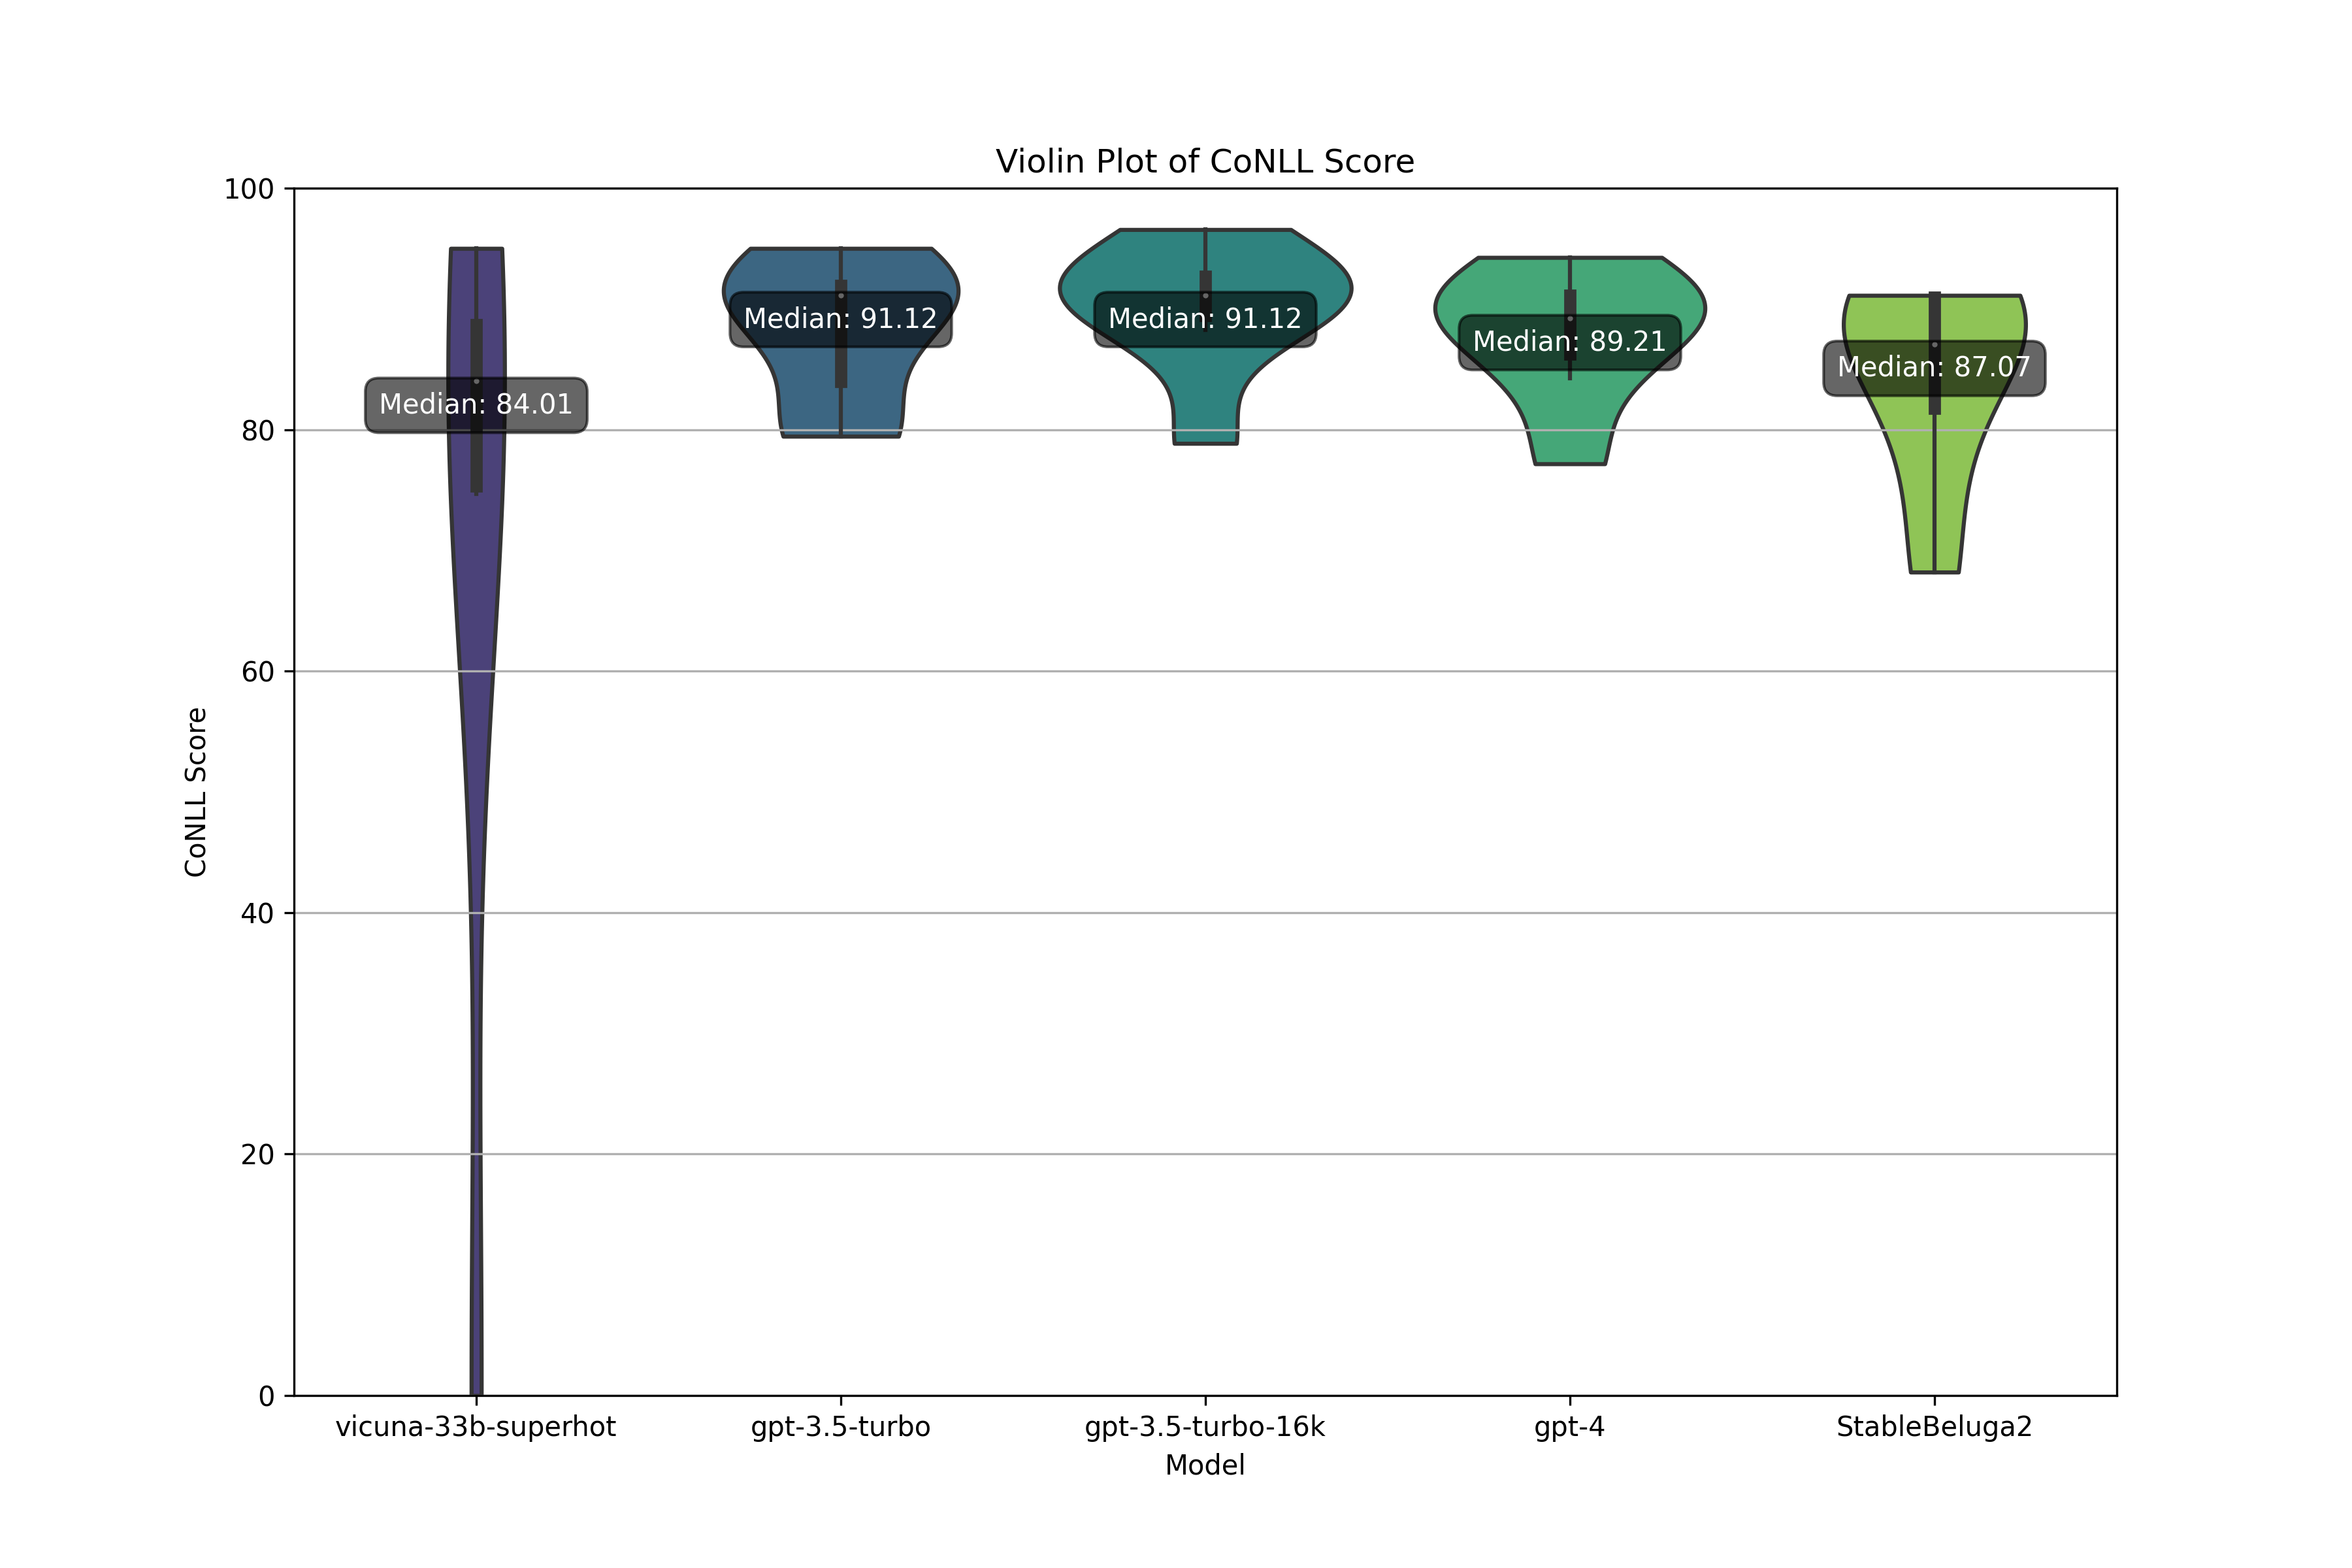
\includegraphics[width=14cm]{images/open-conll-score.png}
  \end{tabular}
  \caption[CoNLL Score Open Source]{Violin Plot of the CoNLL scores using all 5 models}\label{fig:open-source-conll}
\end{figure}

\subsection{Coverage of Annotation}

Once again, vicuna-33b faced challenges in providing complete coverage for one paper, resulting in one score of zero. StableBeluga2, on the other hand, achieved performances comparable to the GPT Models, as can be seen in Figure~\ref{fig:open-coverage}. Even disregarding the isolated zero score for Vicuna-33b, its performance generally remains subpar compared to its more advanced counterparts. 

\begin{figure}[htpb]
  \centering
  \begin{tabular}{c}
  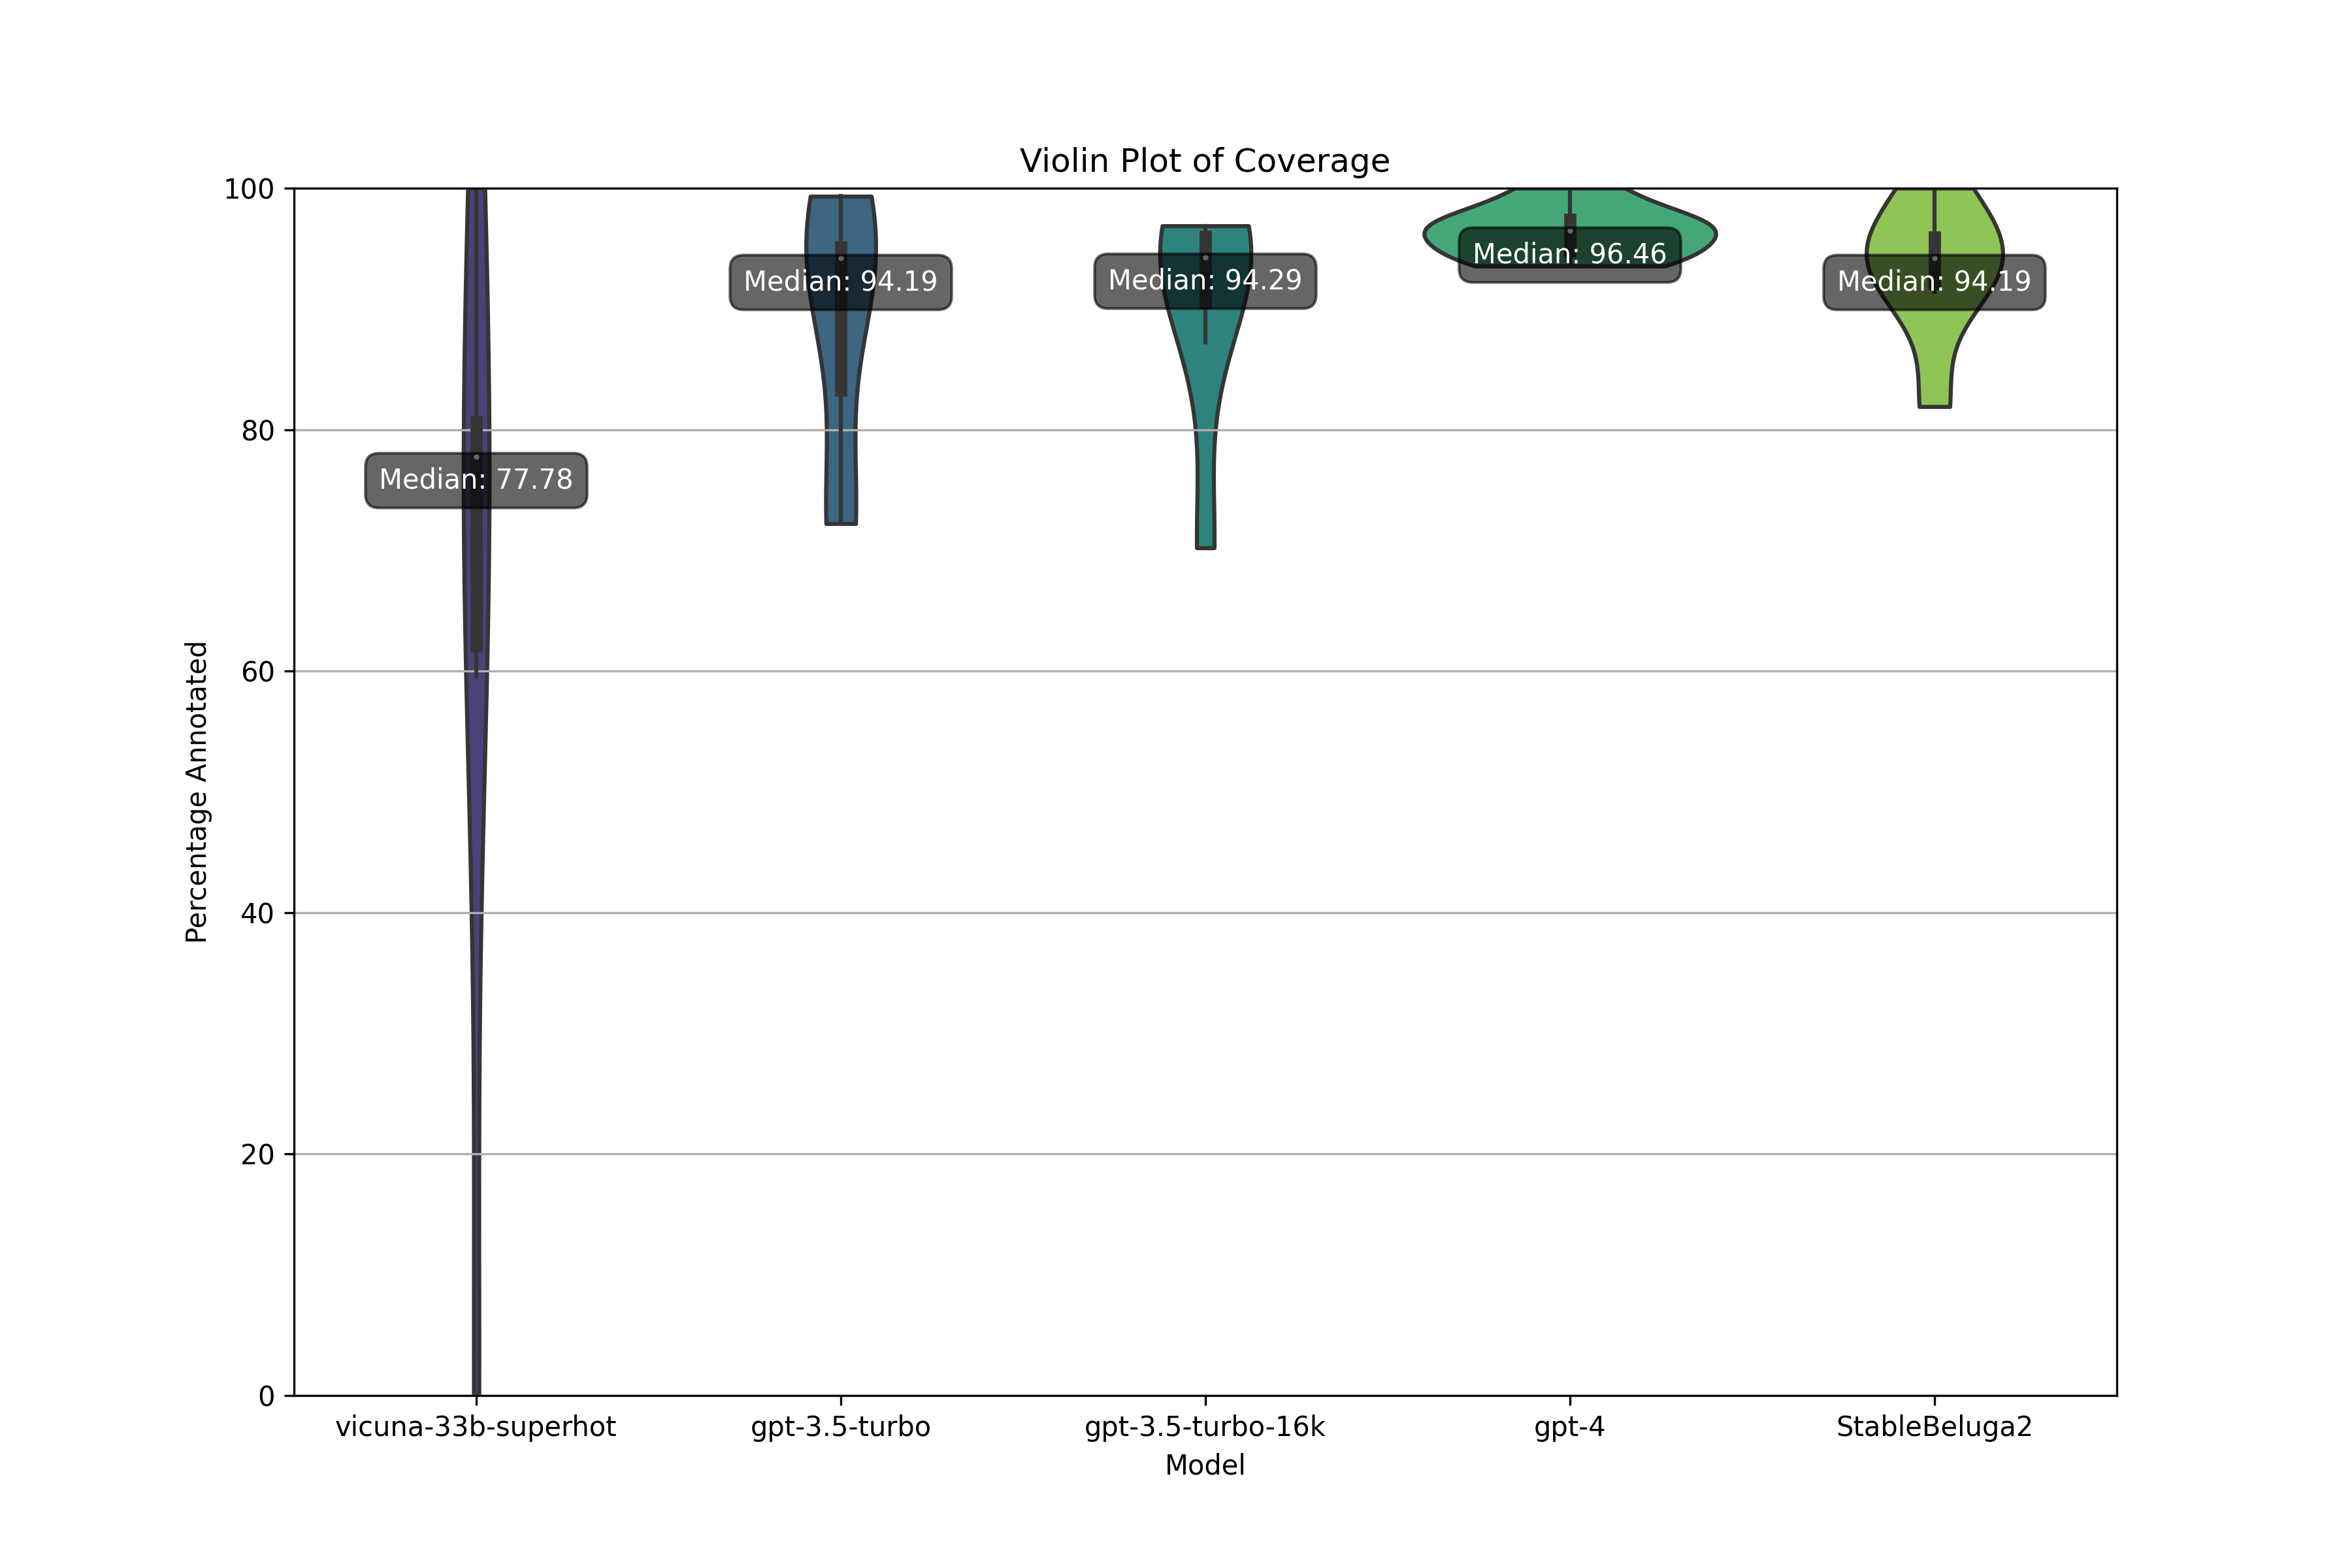
\includegraphics[width=14cm]{images/open-coverage.png}
  \end{tabular}
  \caption[Open Source Coverage]{Violin plot of the coverage of the 7 papers annotated}\label{fig:open-coverage}
\end{figure}

\subsection{Semantic Accuracy}

Semantic accuracy is the cornerstone of our comparative study. Due to the labour-intensive nature of manual evaluation, we selected a subset of six papers for this purpose. StableBeluga2, an OpenSource LLM, beats GPT-3.5 entirely but could not surpass GPT-4, which deserves mention due to the unmatched complexity and sophistication of GPT-4's architecture. As shown in Figure~\ref{fig:open-semantic}, the comparable performance of StableBeluga2 and the GPT models reinforces this open-source model's potential to accurately understand and reflect the context of scientific papers. Vicuna-33b's performance was notably lacklustre, a limitation likely attributable to its smaller model size.

\begin{figure}[htpb]
  \centering
  \begin{tabular}{c}
  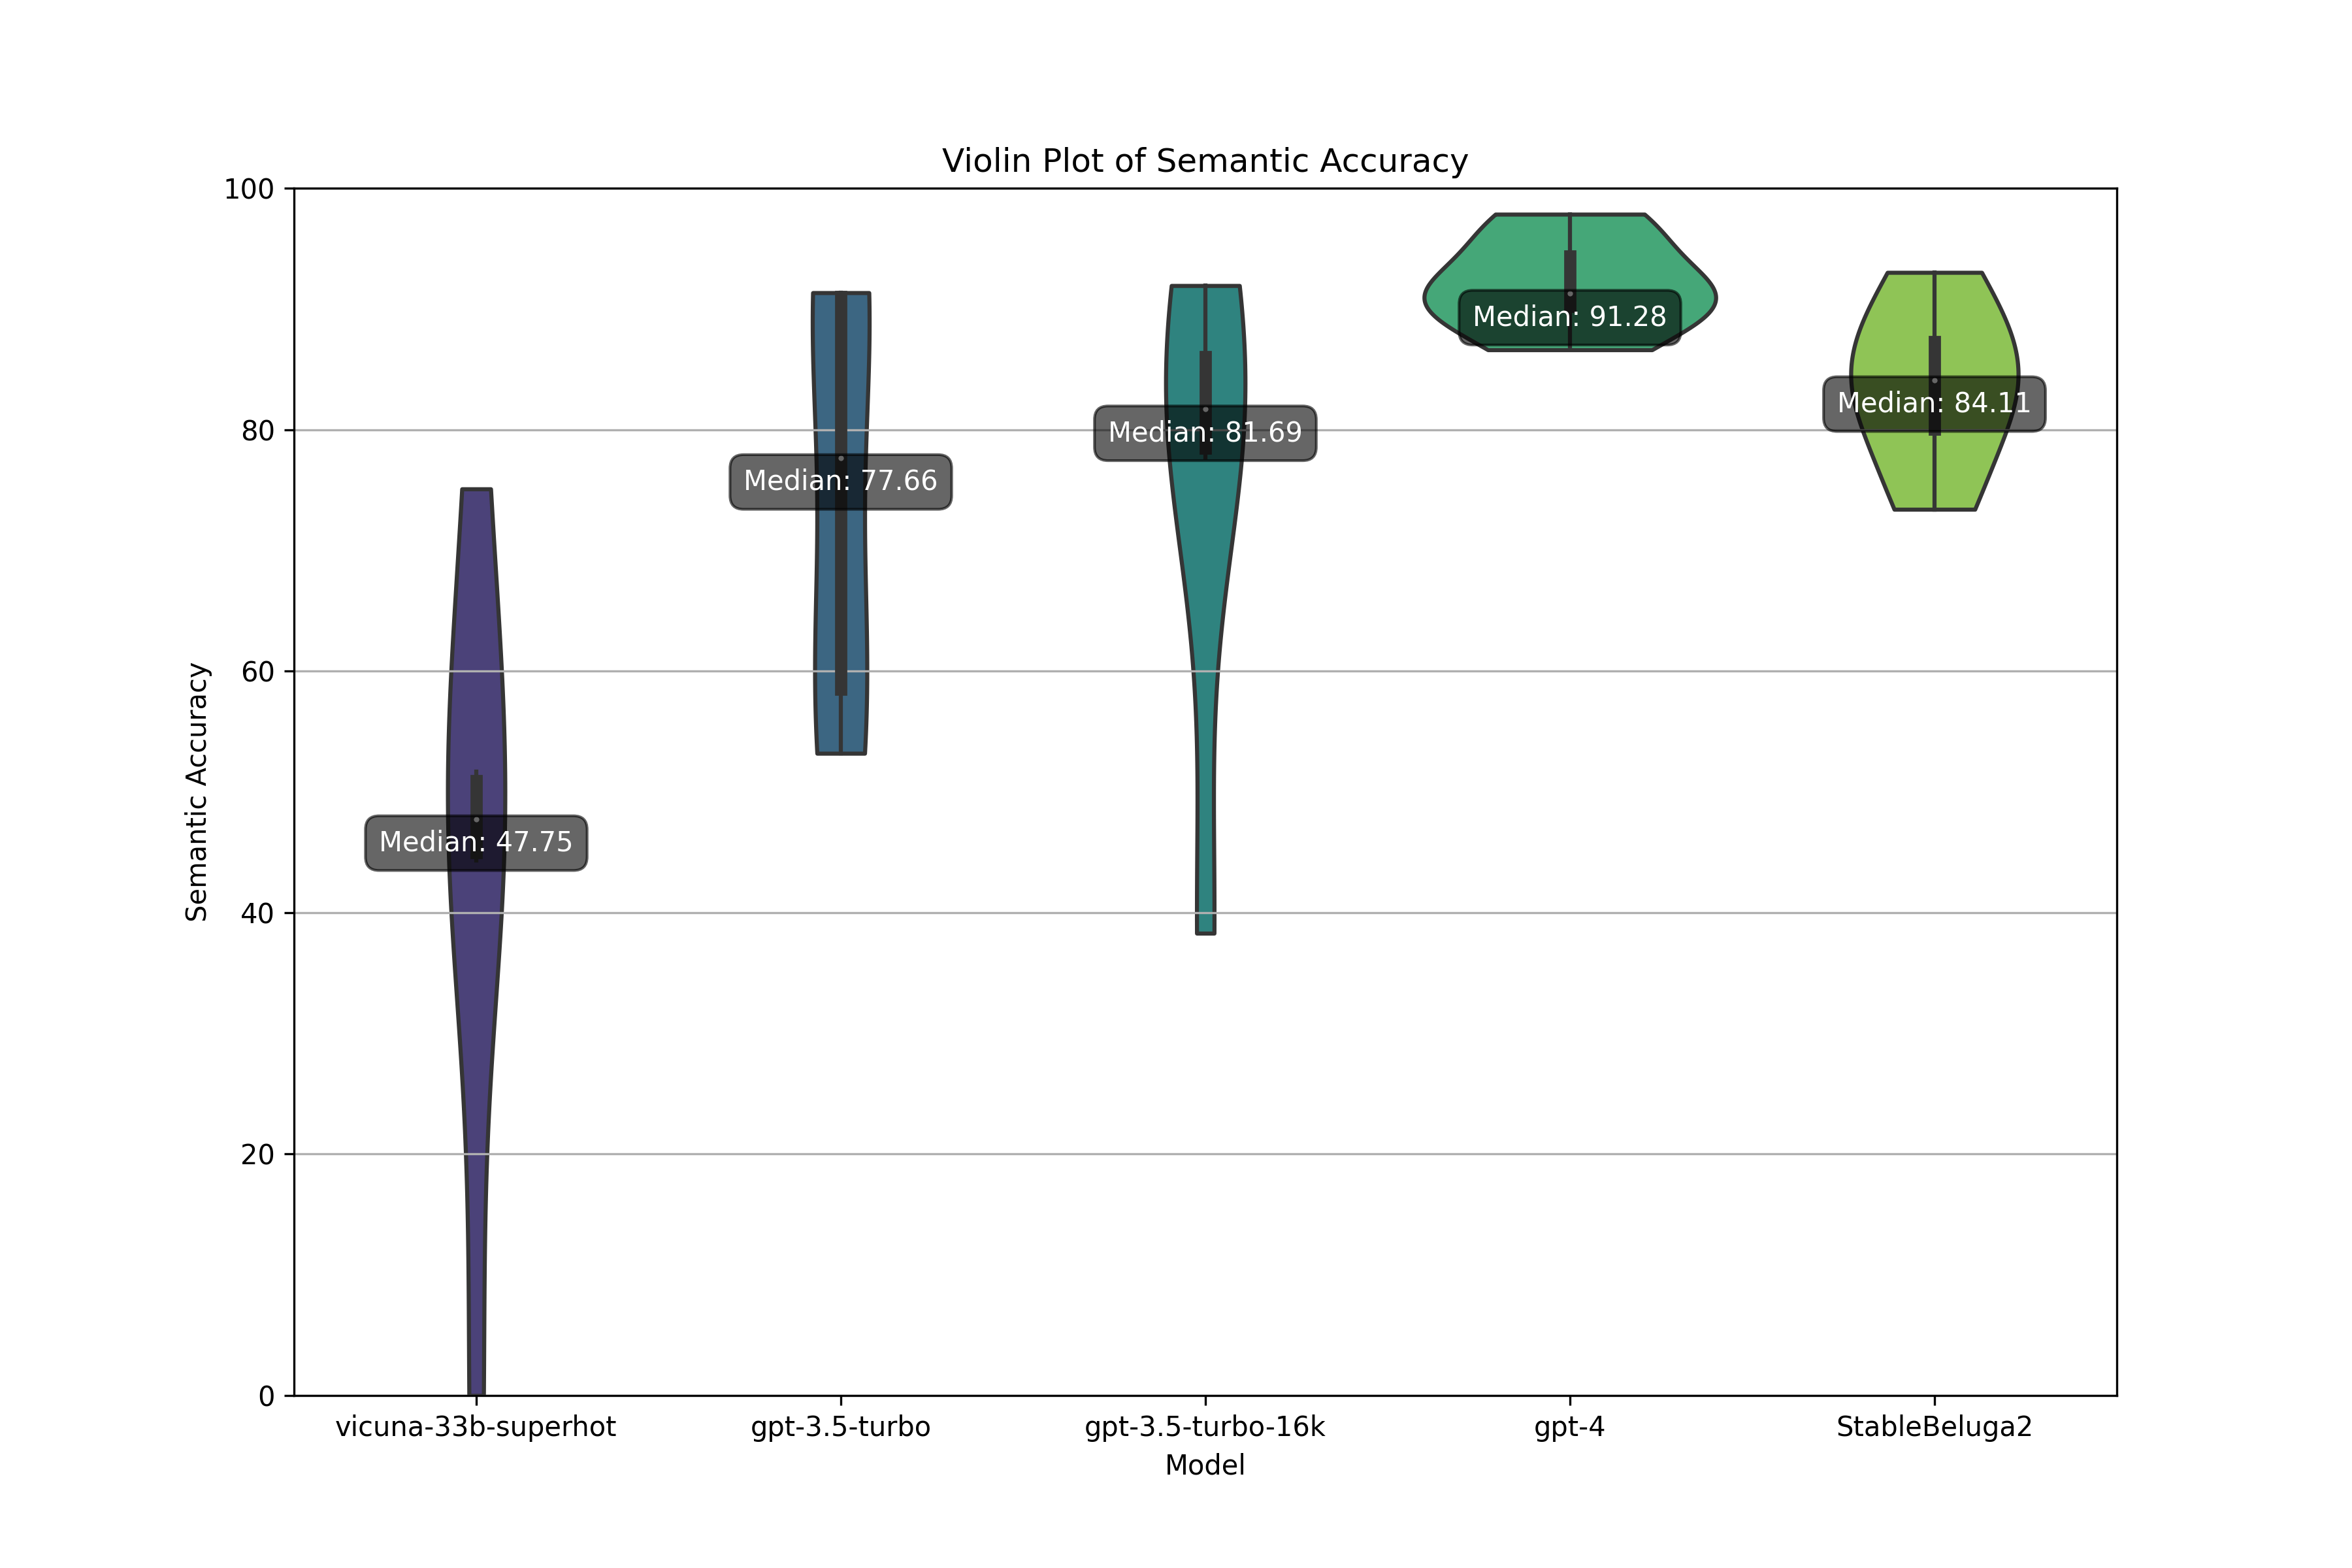
\includegraphics[width=14cm]{images/open-semantic.png}
  \end{tabular}
  \caption[Semantic Accuracy]{Semantic Accuracy Scores from all the five models on six papers}\label{fig:open-semantic}
\end{figure}

\subsection{Running Time and Costs}

%Given the distinctive operational requirements of open-source models, t %% Repetition from Chap 4.
The computation of time and cost differ between open-source and GPT models. Unlike GPT models, the cost for open-source models revolves around GPU run-time cost (in our case, on the servers of \href{https://runpod.io}{runpod.io}) and not token usage. The running time is visualised in Figure \ref{fig:open-runtime}. However, since the time taken here depends on the length of the paper, it is essential to compare the costs per annotation. This can be visualised in \ref{fig:open-relative-cost}. Because of cheaper hardware, the average run time of open-source LLMs was prolonged. On average, they were 5-10x slower. This is especially noticeable for StableBeluga2 as it is a reasonably large LLM. The cost for the experiments can differ from person to person, based on their machinery. We had to pay for the GPU usage, but if a person owns GPUs, it can be "free of cost". Regardless, we have visualised the cost we paid for annotations in Figure~\ref{fig:open-cost}. It can also very well happen that the cost to use these GPUs is higher than for GPT tokens. GPT-4 is significantly more expensive than all other models. vicuna-33b has a similar operating cost to GPT-3.5 but performs way worse. StableBeluga2, which performs better than GPT-3.5, costs 3x more than GPT-3.5 and 3x less than GPT-4.

\begin{figure}[htpb]
  \centering
  \begin{tabular}{c}
  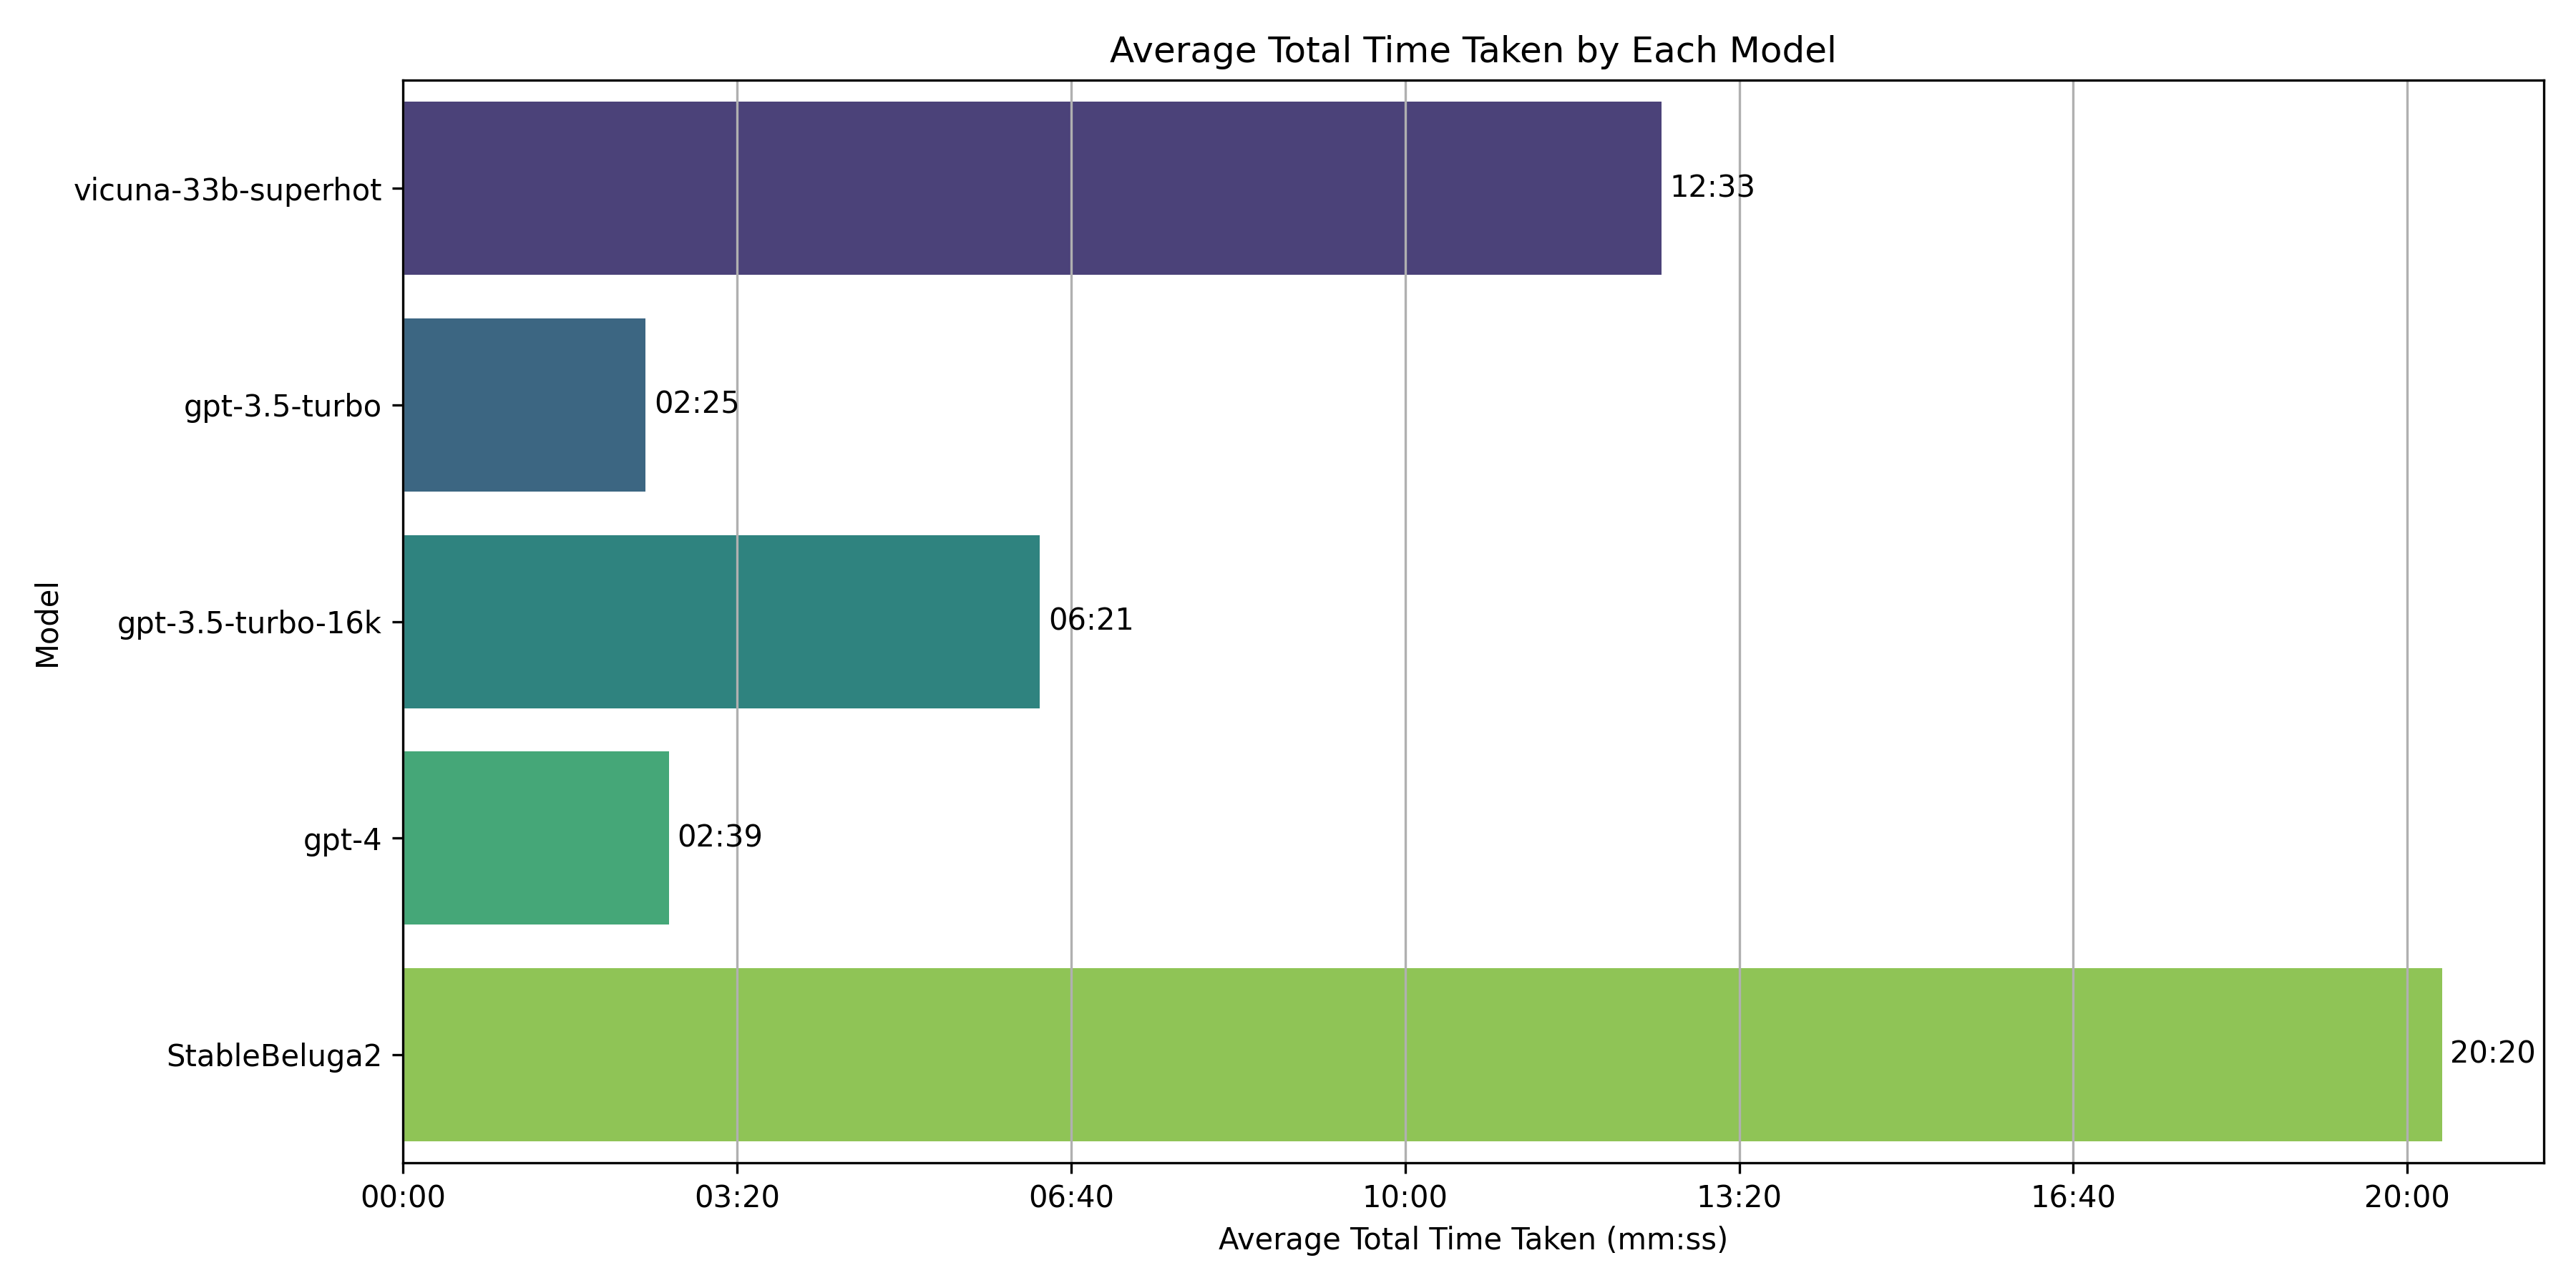
\includegraphics[width=14cm]{images/open-runtime.png}
  \end{tabular}
  \caption[Open Source Time]{Average Time Taken by all five models on six papers}\label{fig:open-runtime}
\end{figure}

\begin{figure}[htpb]
  \centering
  \begin{tabular}{c}
  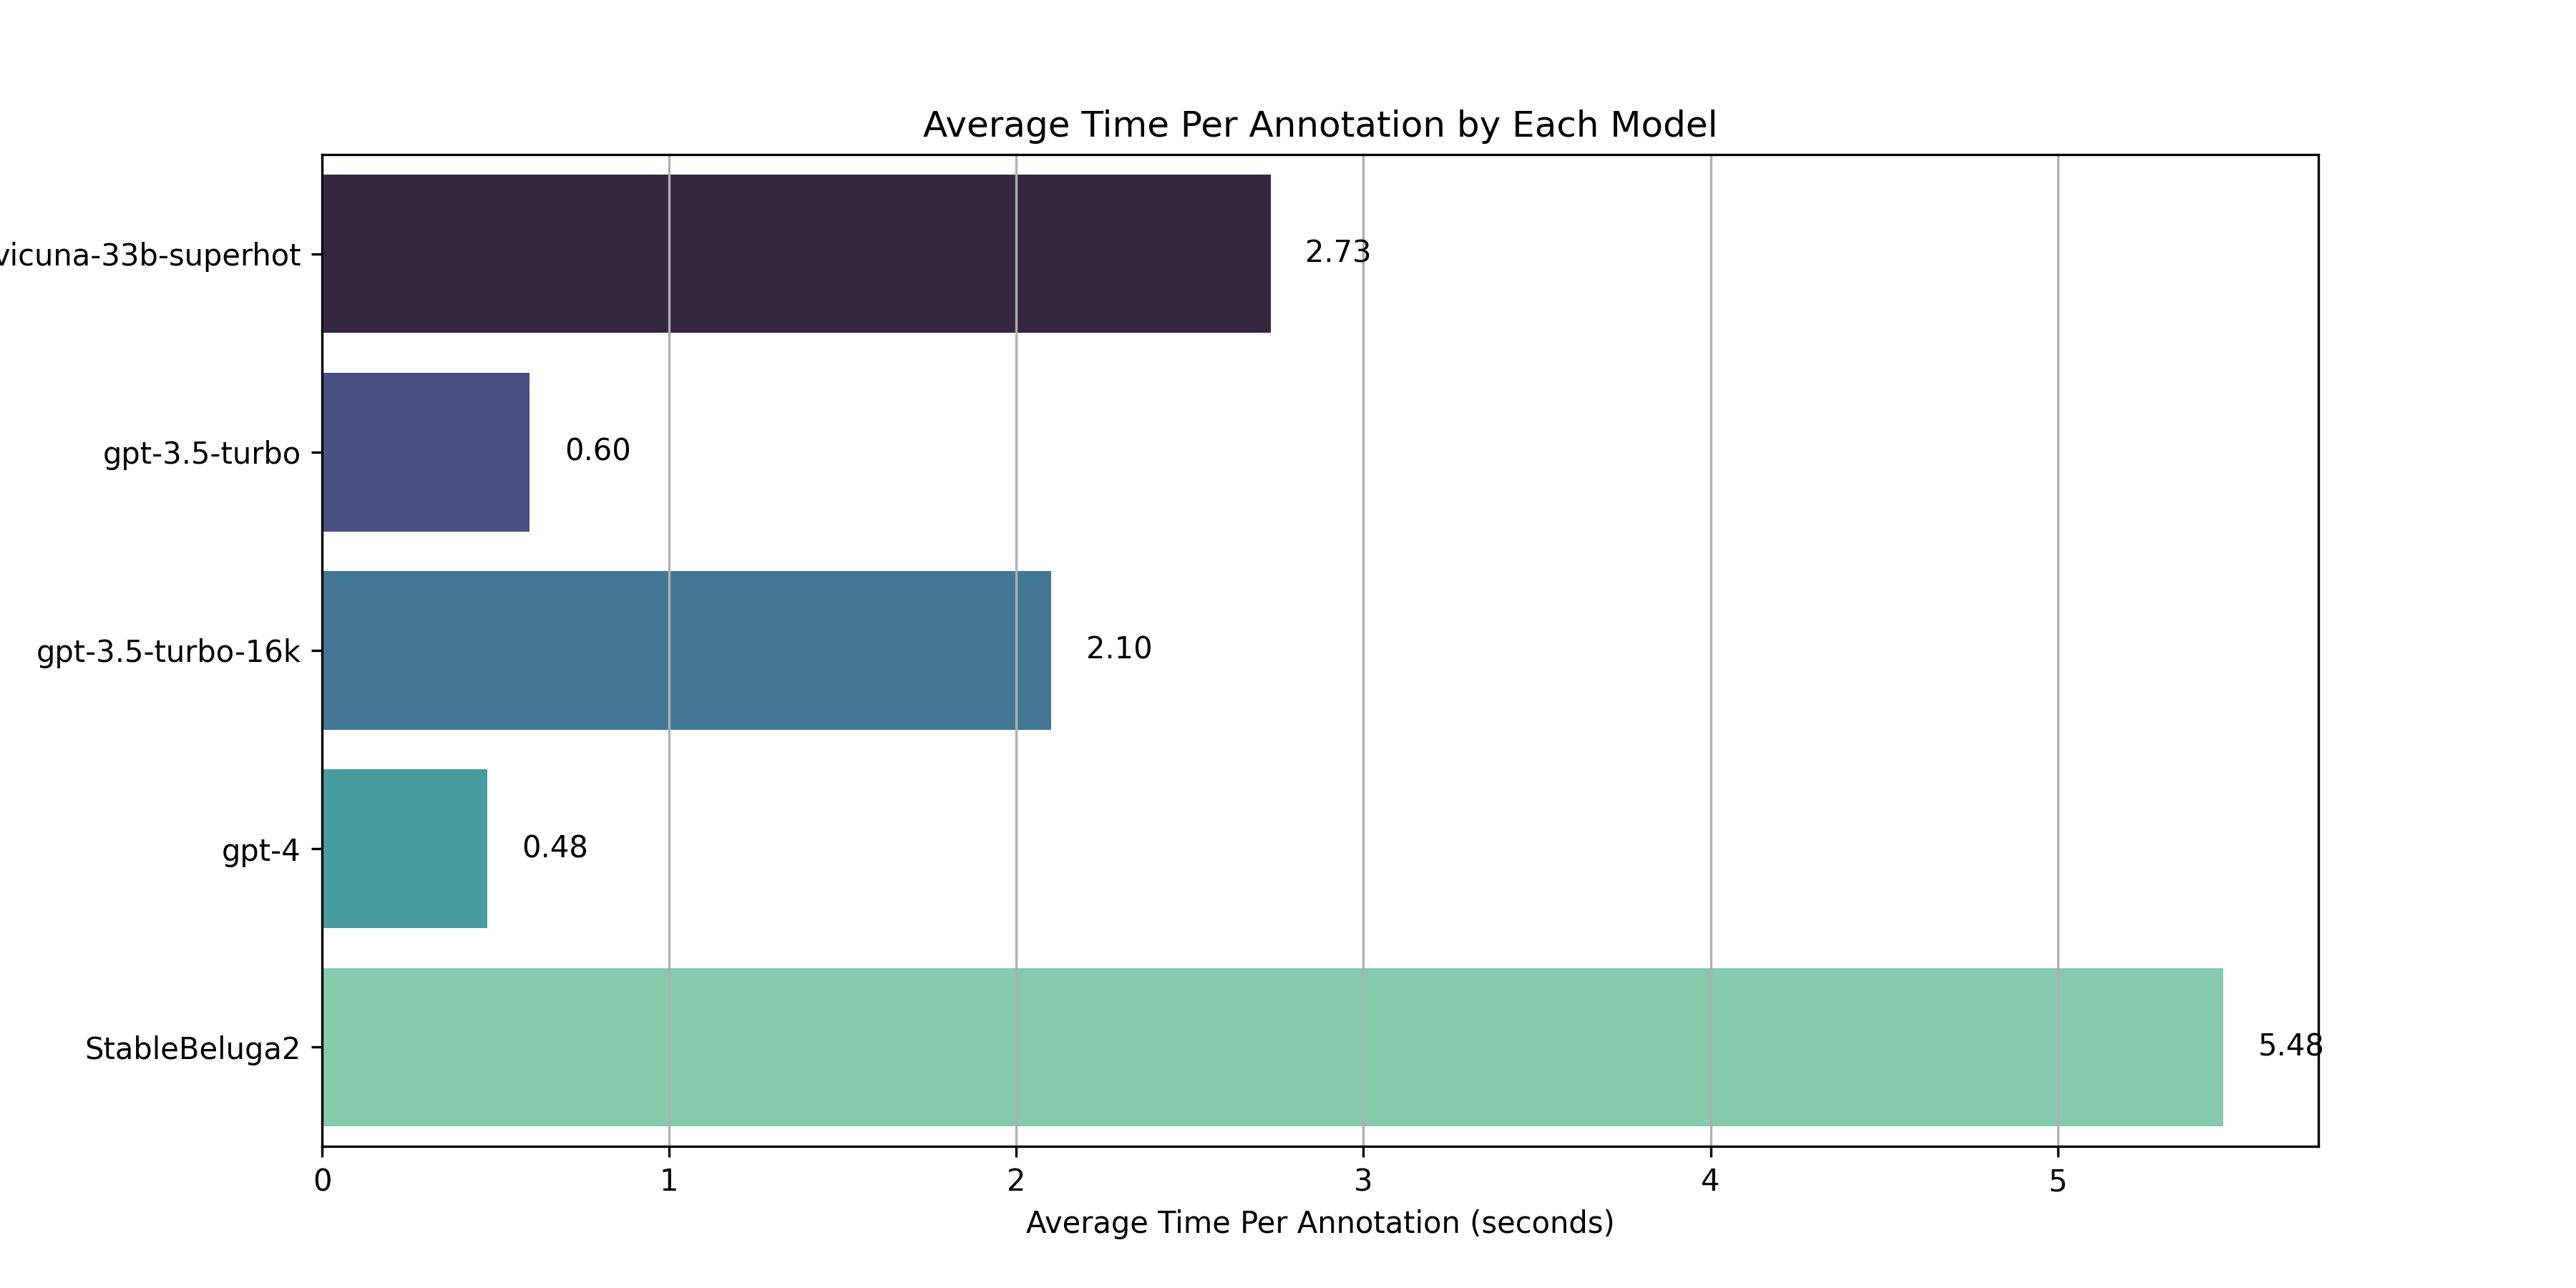
\includegraphics[width=14cm]{images/open-anno-cost.png}
  \end{tabular}
  \caption[Open Source Cost]{Average Time Taken Per Annotation by all five models on six papers}\label{fig:open-relative-cost}
\end{figure}

\begin{figure}[htpb]
  \centering
  \begin{tabular}{c}
  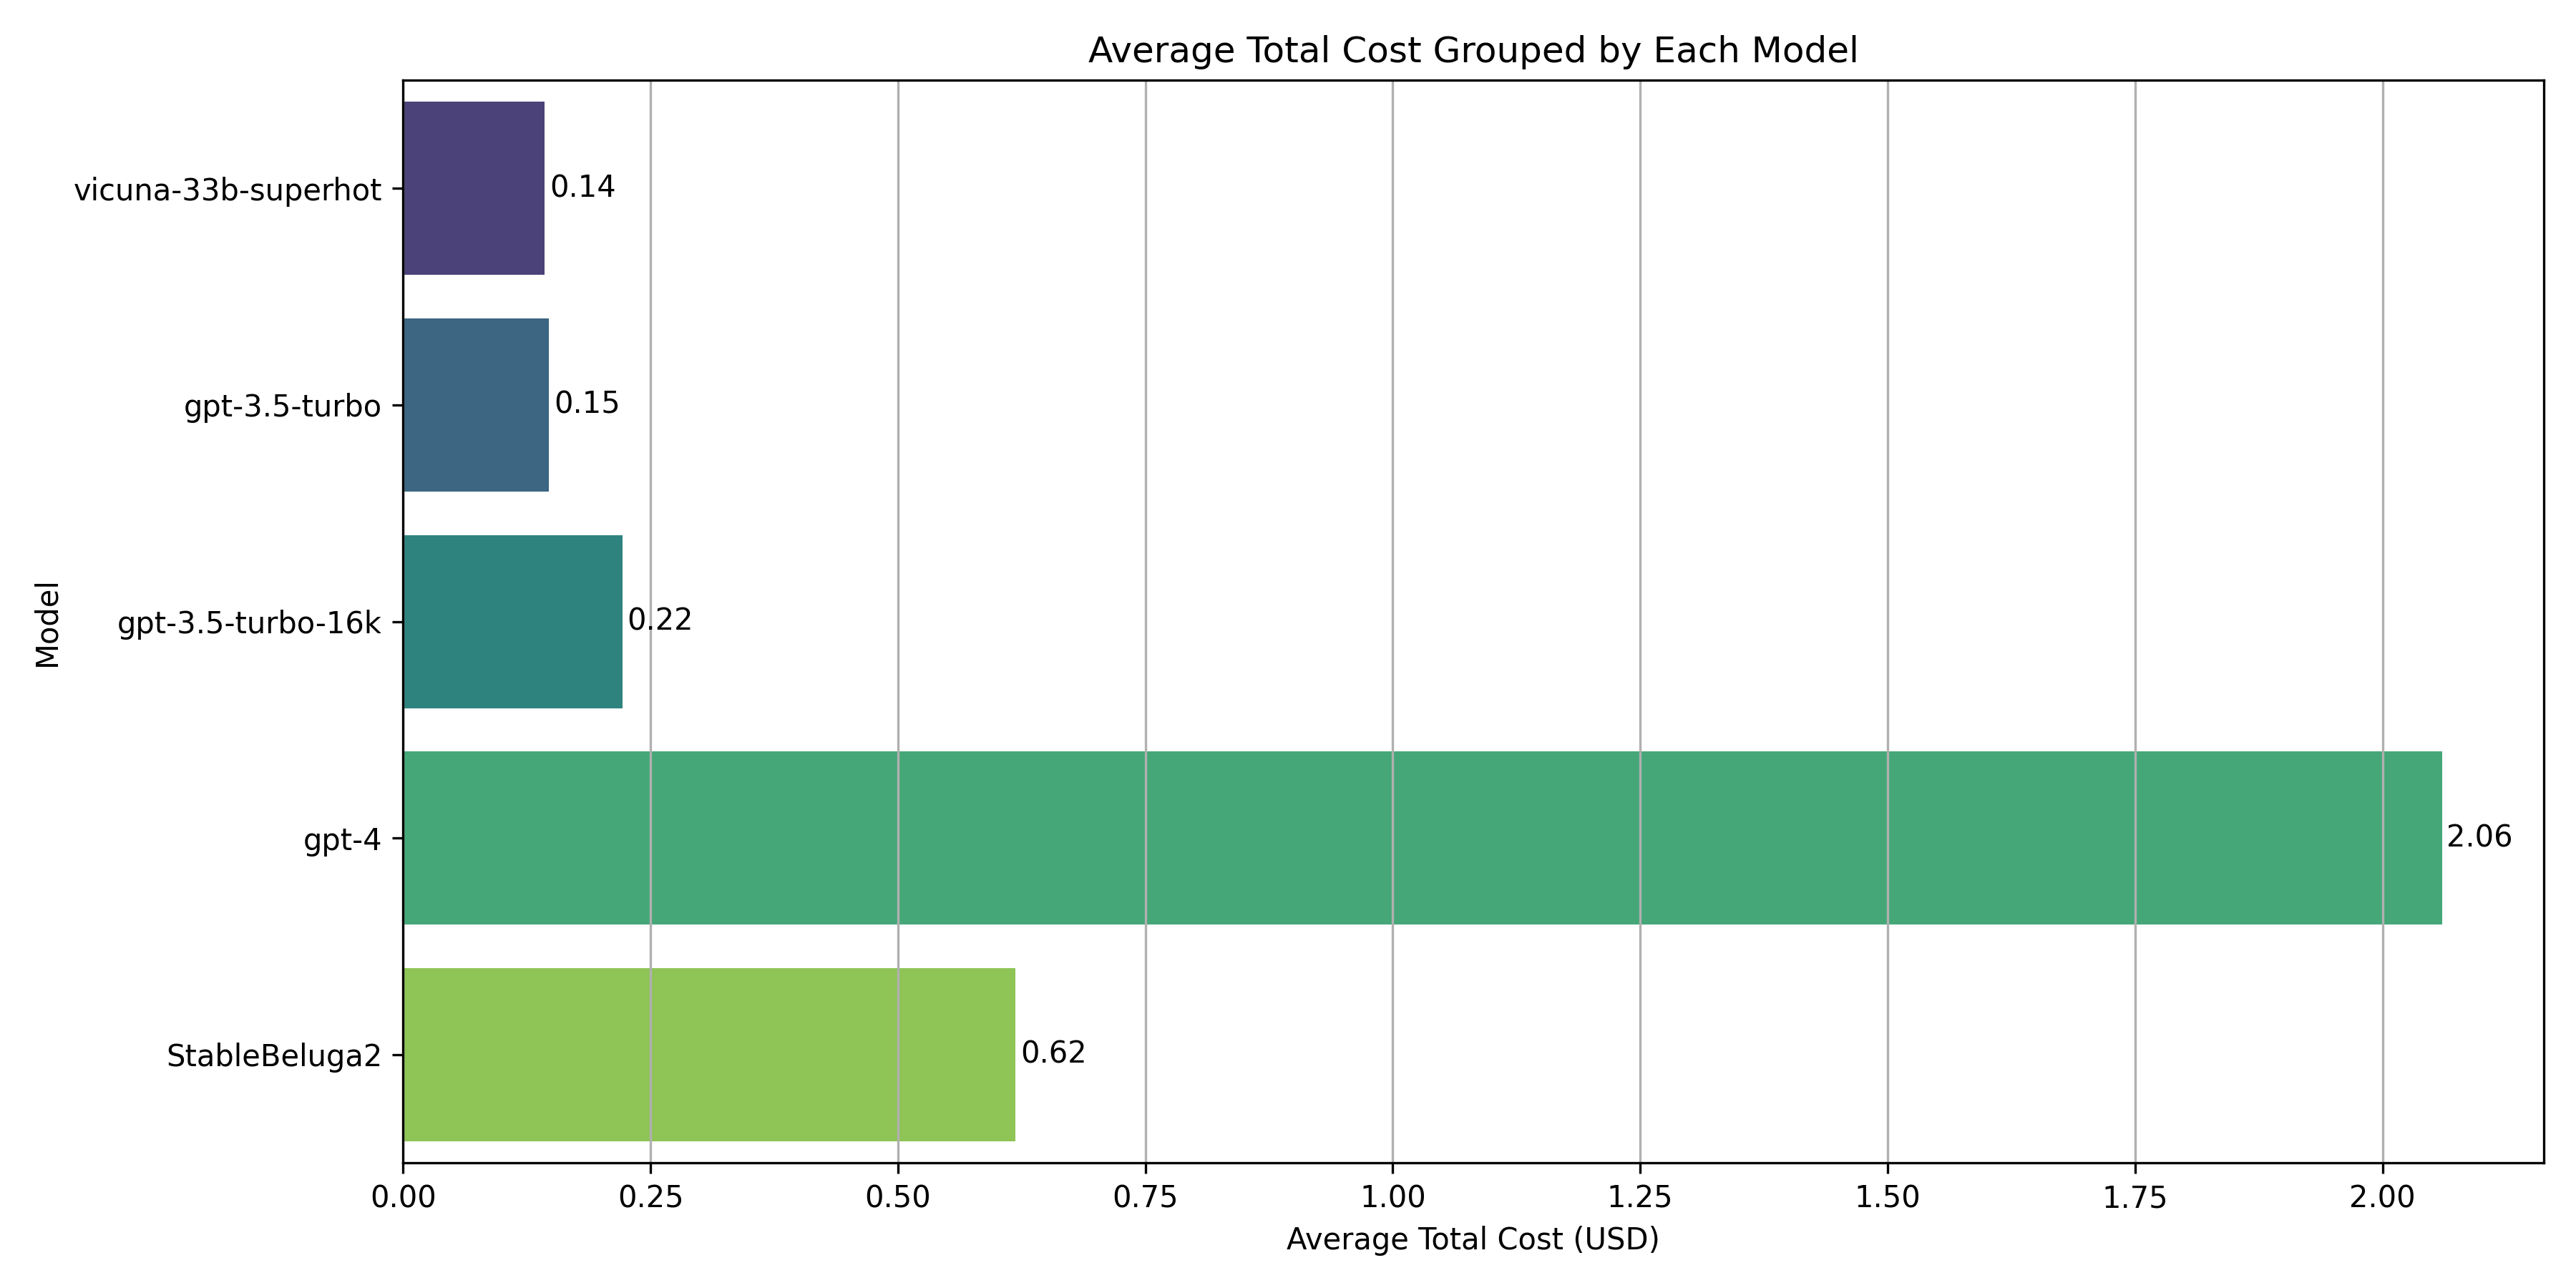
\includegraphics[width=14cm]{images/open-cost.png}
  \end{tabular}
  \caption[Open Source Time]{Average Paid Cost by all five models on six papers}\label{fig:open-cost}
\end{figure}

\section{Evaluating Potential Correlations}

Upon completion of our results assessment, it was fundamental to investigate potential correlations inherent in the results. We probed two areas of interest: a potential correlation between the CoNLL Score and Semantic Accuracy and a possible linkage between the CoNLL Score and the paper's publication date. These examinations were crucial to determine whether any part of the original paper was contained within OpenAI's training data.

%% THIS IS HOW FAR I GOT, but I can still read more tomorrow if it is helpful. Cheers!

\subsection{Connection Between CoNLL Score and Semantic Accuracy}

Given that these two metrics reflect distinct facets of the paper, we anticipated that little to no correlation would be discernible. Nevertheless, several statistical measures were employed to thoroughly evaluate this potential relationship: Pearson's Correlation Coefficient, Spearman's Rank Correlation, and Kendall's Tau. As seen in Table \ref{tab:spearman}, the correlation results indicate a trivial association between these metrics, as the correlation constant is virtually zero, supported further by a notable high p-value.

\begin{table}[htpb]
    \centering
    \caption{Correlation Coefficients and P-values}\label{tab:spearman}
        \begin{tabular}{lrr}
        \hline
        Method & Correlation & P-value \\
        \hline
        Pearson's Correlation Coefficient & -0.1570 & 0.5472 \\
        Spearman's Rank Correlation & -0.0006 & 0.9981 \\
        Kendall's Tau & -0.0075 & 0.9670 \\
        \hline
    \end{tabular}
\end{table}

\subsection{Influence of Publish Date on CoNLL Score}

A query was raised regarding the possibility of papers released before September 2021—presumed to be the cut-off date for building OpenAI's GPT Models training data—yielding higher CoNLL Scores than those published afterwards. The difference in average CoNLL scores between papers released before was higher by 1.63 compared to those released after the cut-off date. This might be attributable to the variable nature of LLMs rather than the inclusion in the training set. For post-cut-off papers, the semantic accuracy was also marginally lower—by an average of 5.87\%. However, this difference did not significantly suggest being due to training data influence.
Furthermore, the use of GPT to generate novel annotations makes it improbably likely for these exact or similar outputs to exist in the training dataset and affect the results. An observation worthy of mention is that the post-2021 papers contained significantly more concepts, which may have influenced the score. Henceforth, it is reasonable to conclude that a paper being part of the training dataset or not does substantially impact the score.

\section{Overall}

In comprehensive terms, GPT-4 emerged as the most impressive model due to its superior performance, albeit at a higher cost. GPT-3.5 was the most cost-effective and fastest model to operate. All GPT models provided commendable annotations for automation purposes, with the Open Source LLM StableBeluga2 marking a significant breakthrough with its "zero-cost" operation and performance that is almost at par with the GPT models. This is particularly noteworthy, considering StableBeluga2 is a 70 billion parameter model, and GPT-4 is rumoured to be a 1.8 trillion parameter model. The instructive nature of StableBeluga2, as opposed to the general-purpose chat model design of GPT, likely contributed to its performance in formula grounding. Figure \ref{fig:total-anal} visualises the performance-to-cost ratio for all five models, which helps to choose the models for different purposes.

\begin{figure}[htpb]
  \centering
  \subfloat[Average Cost per 1000 Concept]{
    \begin{tabular}{c}
  %\hspace*{-.25cm}
  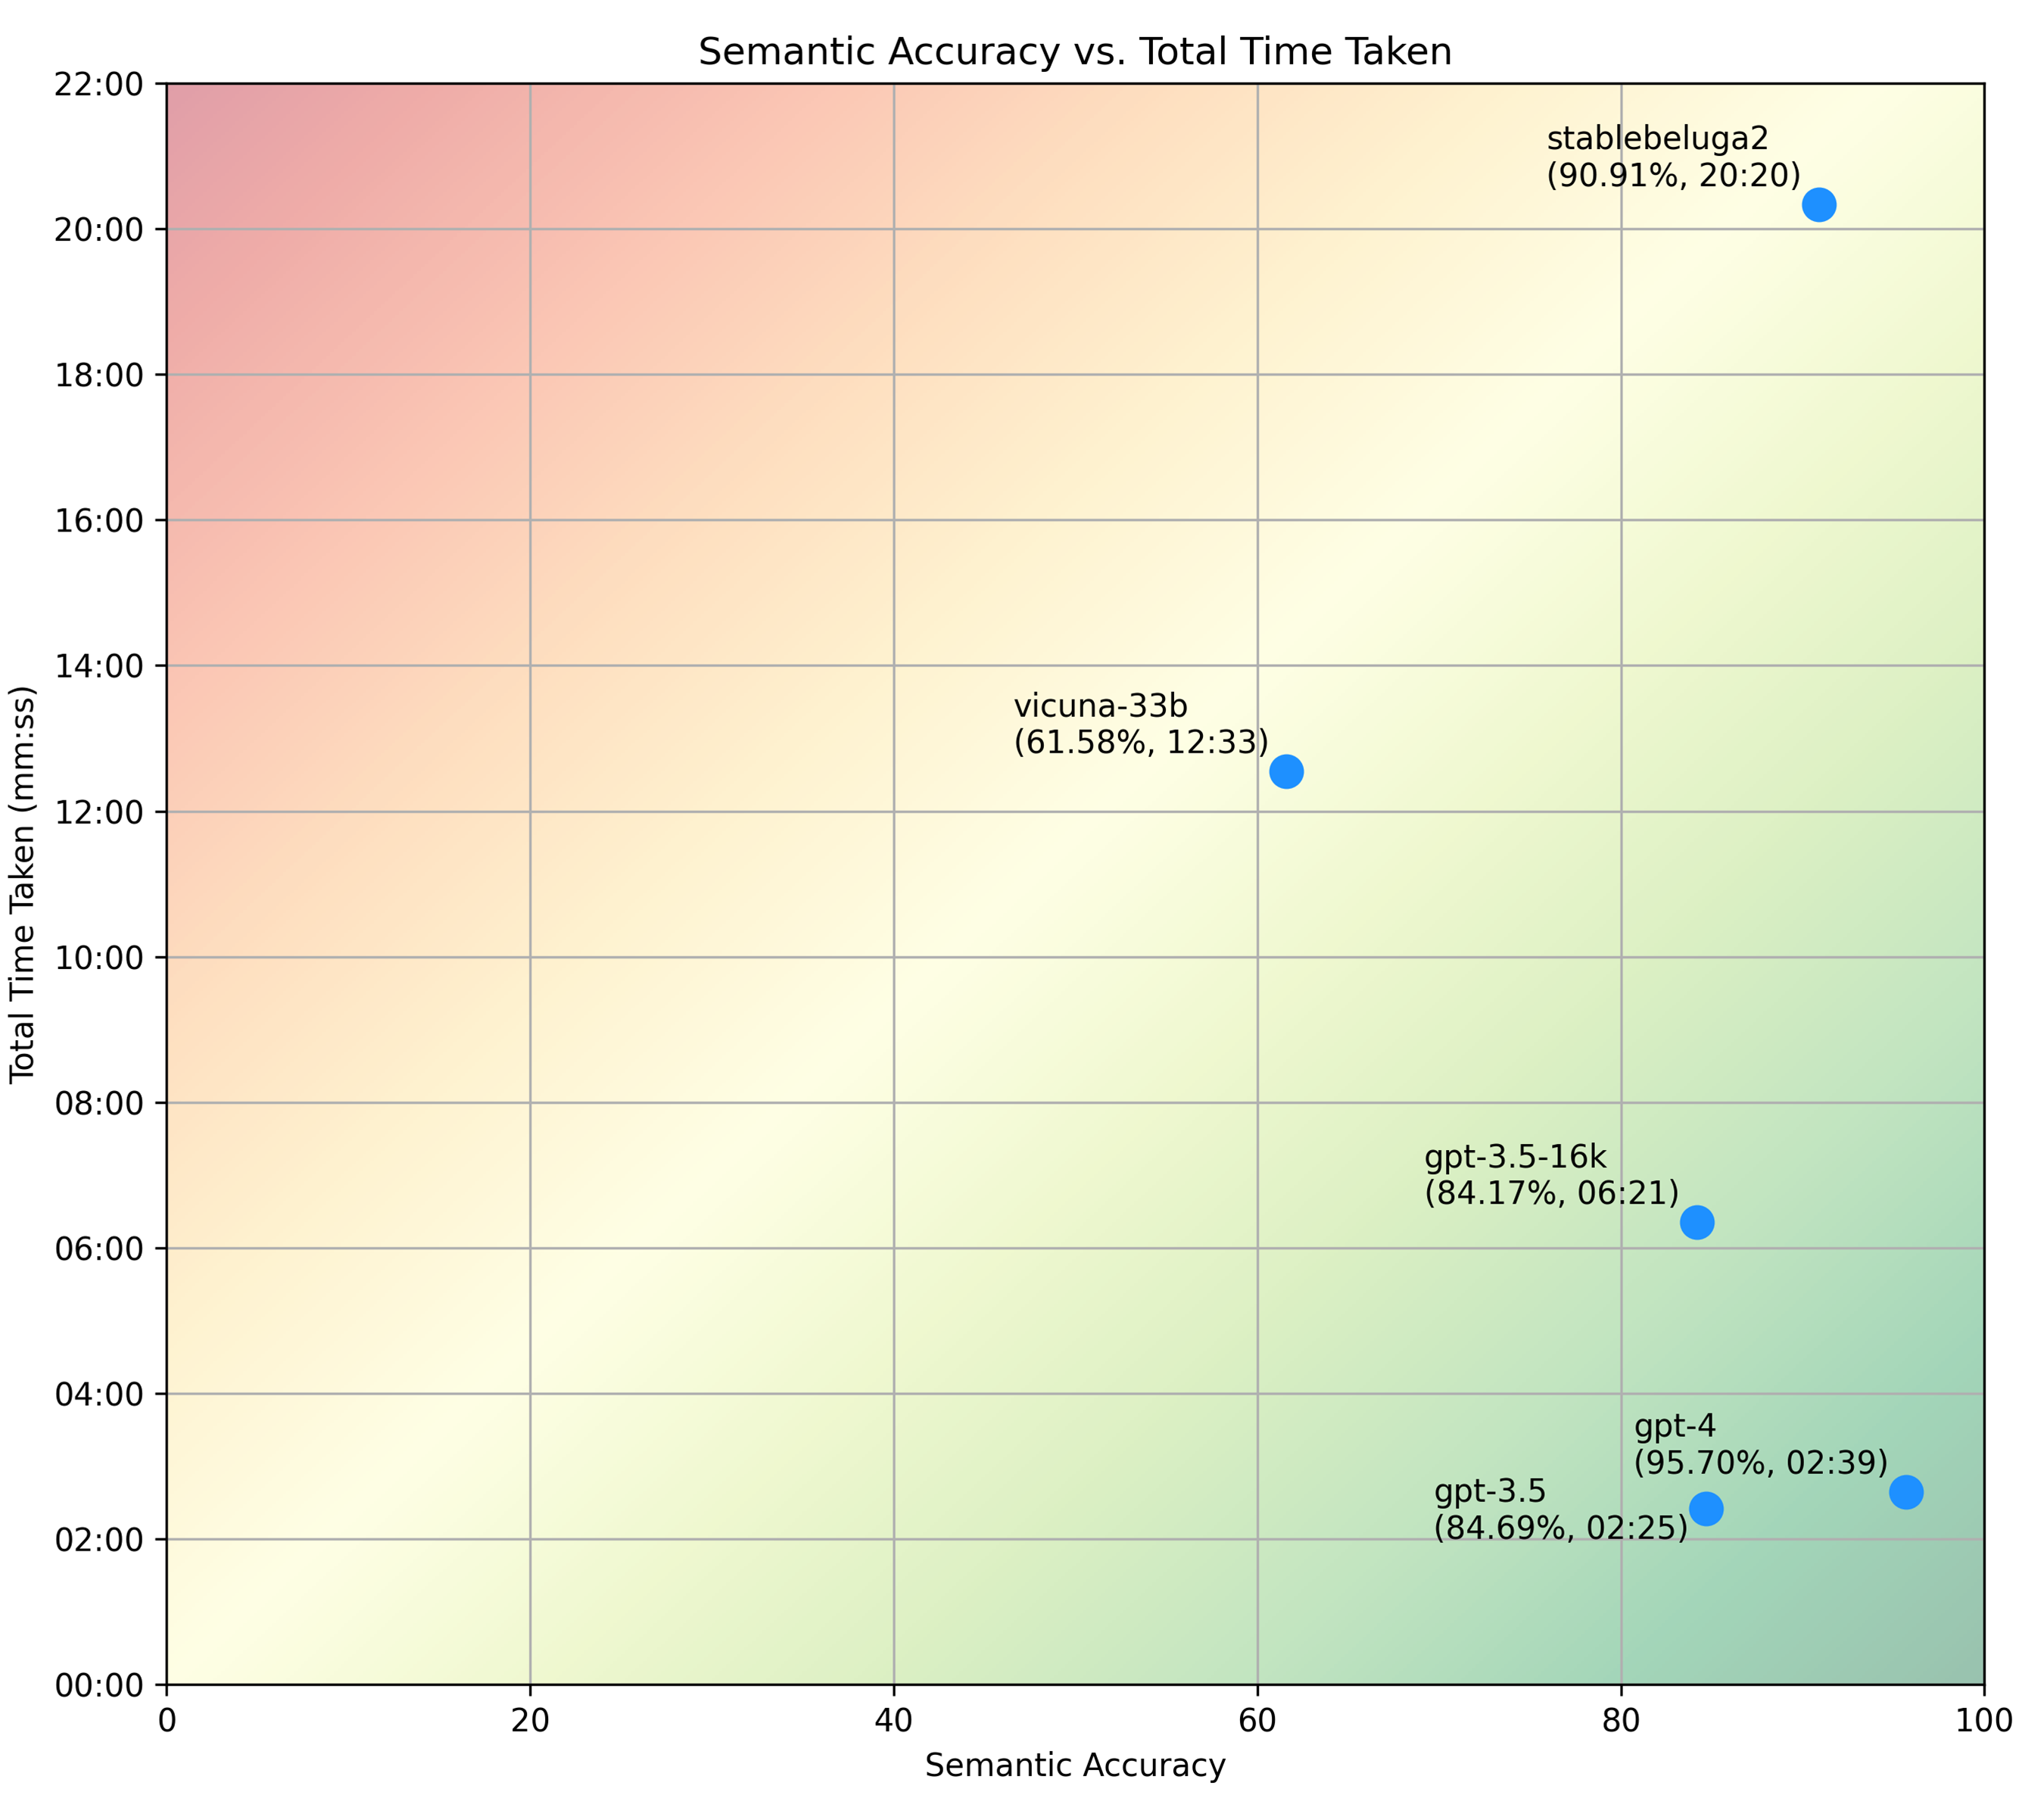
\includegraphics[width=10cm]{images/semantic-time.png}
  \end{tabular}
  }
  \quad 
  \subfloat[Average Duration per Concept]{
    \begin{tabular}{c}
  %\hspace*{-1.5cm}
  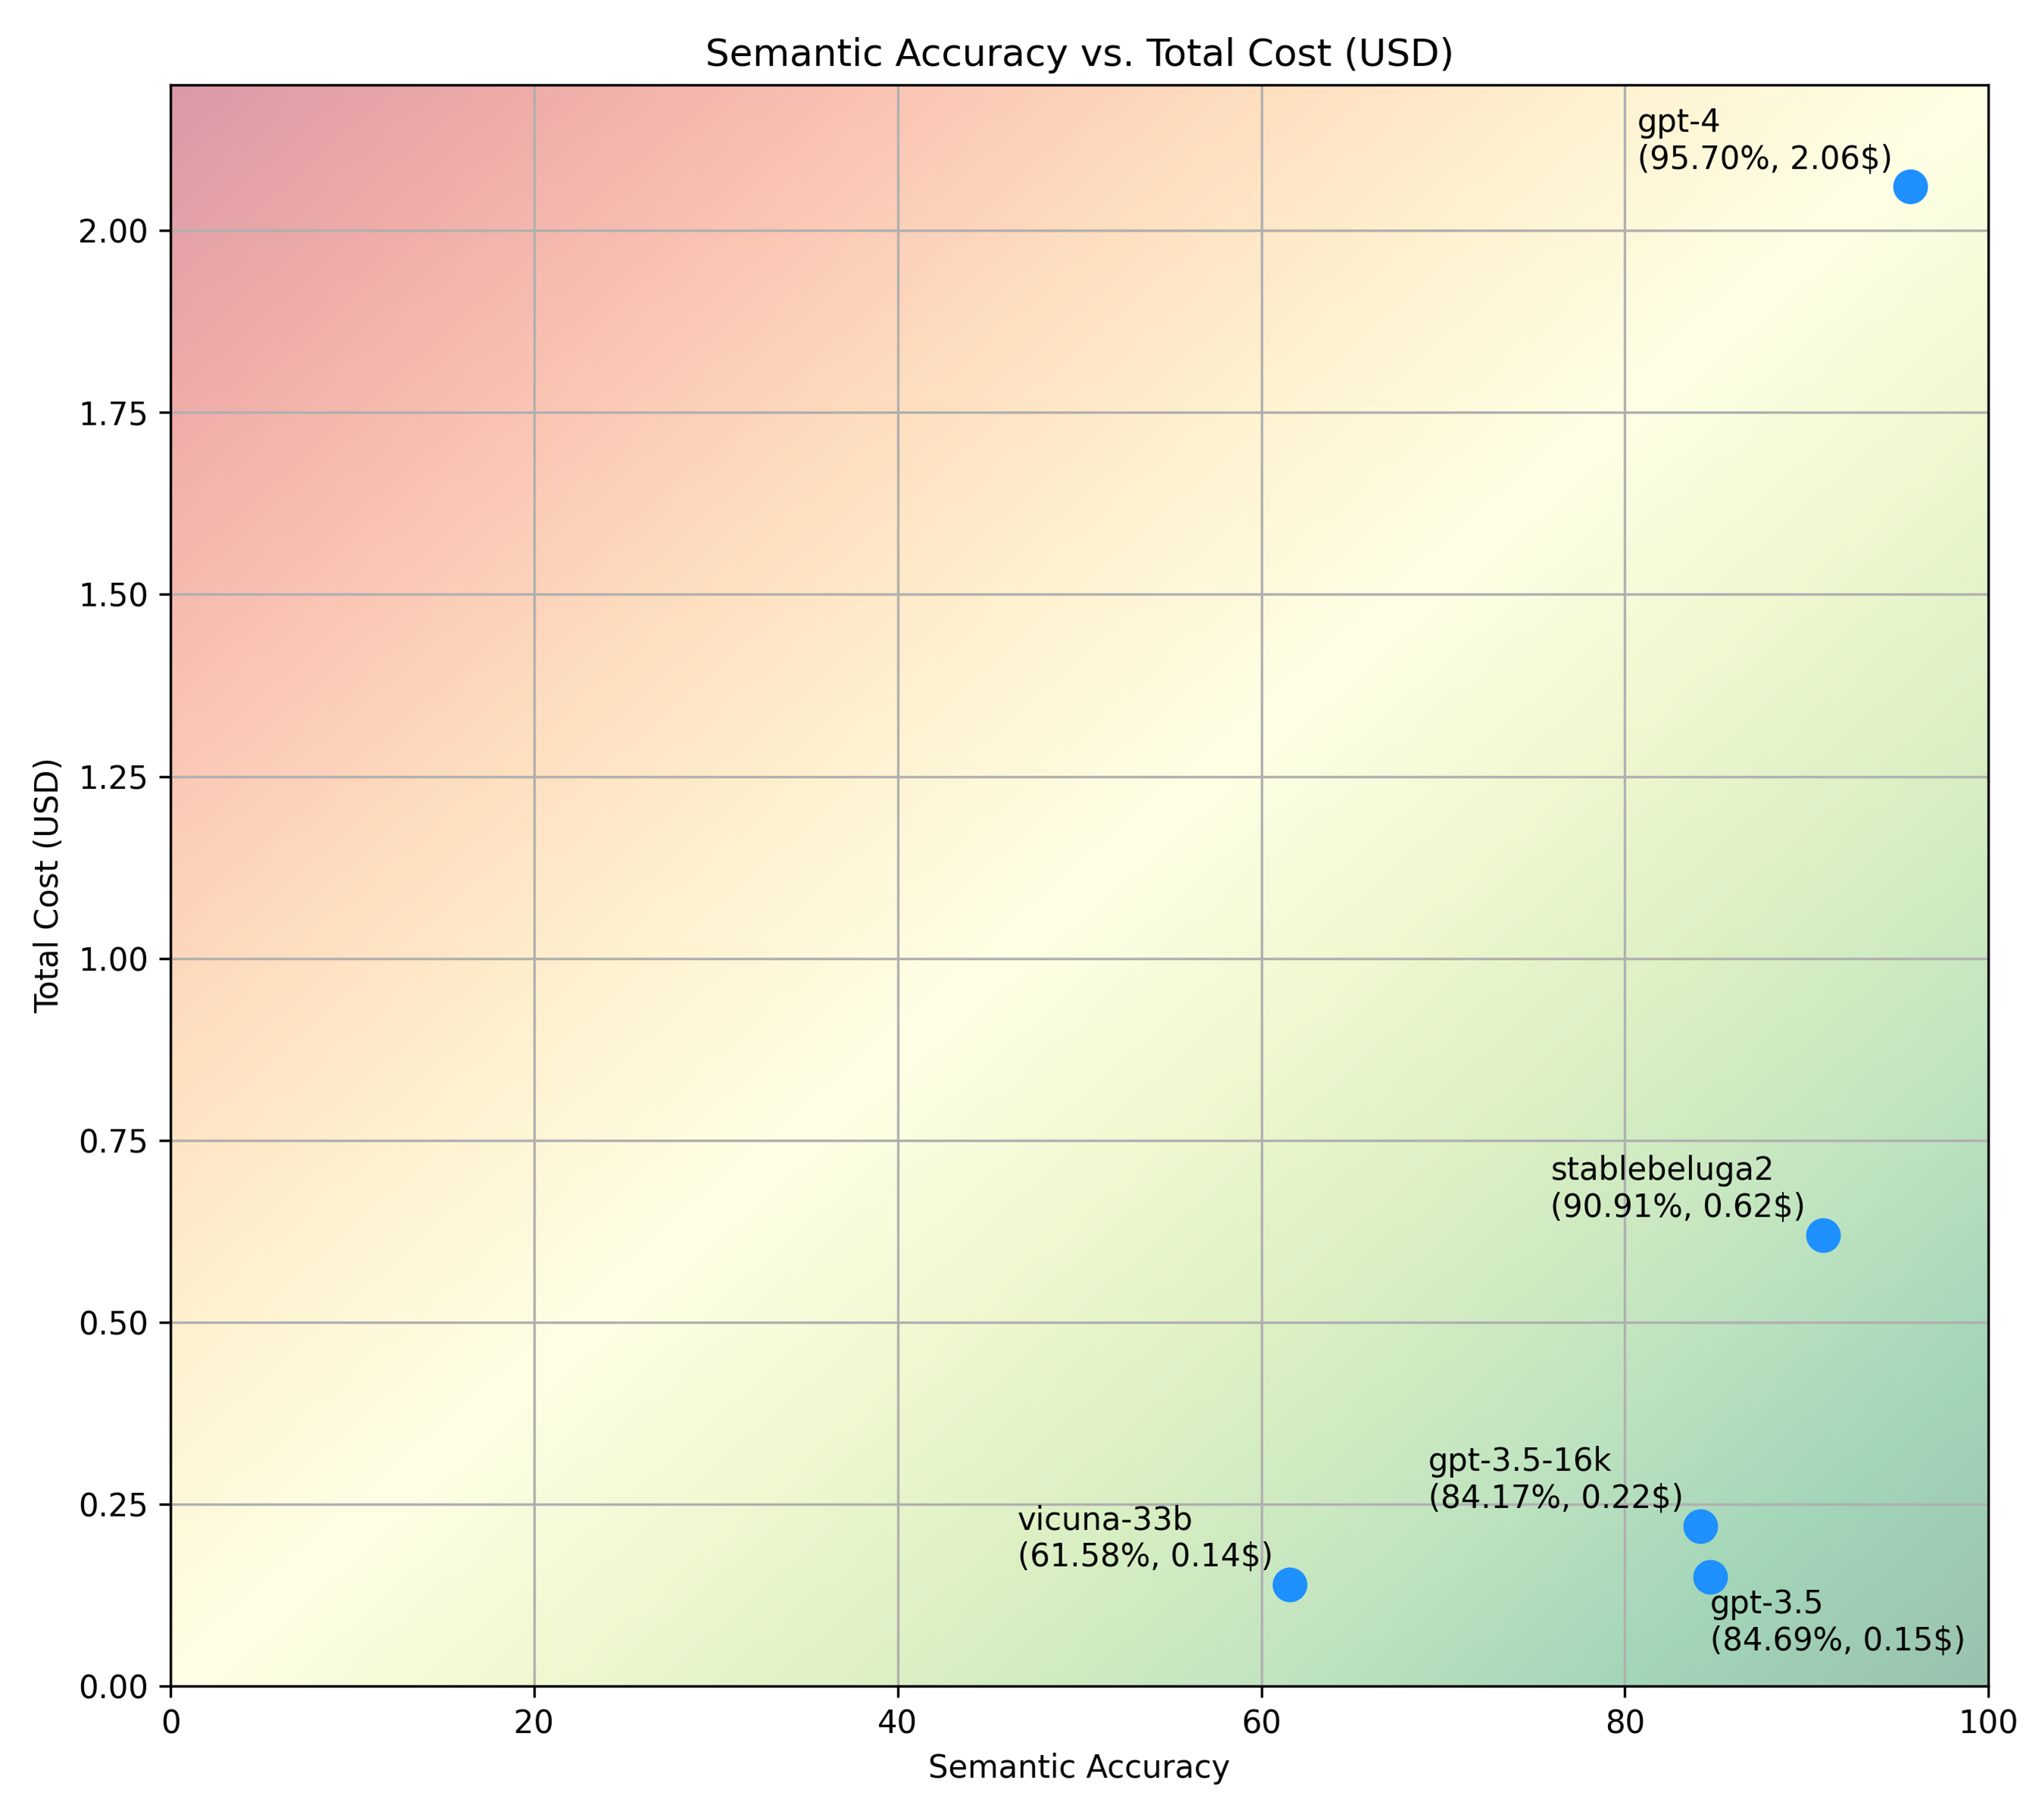
\includegraphics[width=10cm]{images/semantic-cost.png}
  \end{tabular}
  }
  \caption[Cost Analysis]{Cost and Time Usage of Automation}\label{fig:total-anal}
\end{figure}
